% TODO! ajouter cartes avec participation partielle
\documentclass[aspectratio=169,xcolor=dvipsnames, 11pt,mathserif]{beamer} 
\documentclass[aspectratio=169,xcolor=dvipsnames, 11pt,mathserif]{beamer} 

%\documentclass[xcolor=dvipsnames,mathserif]{beamer} % this option has curvier math
%\documentclass[xcolor=dvipsnames,11pt]{beamer}
% Note: the color structure needs to be added here in the title. Now it recognizes all beamer % colors.

%%%%%%%%  PRESENTATION LAYOUT:
\usepackage{appendixnumberbeamer} % this package does not count the appendix pages. /!\ Inconstant behavior, sometimes bug.
\mode<presentation>
{
  \usetheme{Boadilla}
  \usecolortheme{lily} % lily is nice or orchid but not for definition
  \setbeamercovered{invisible}
  \setbeamertemplate{footline}{\raggedleft\insertframenumber~/~\inserttotalframenumber\hspace*{3pt}\vskip3pt} %this command shows frame number, not page number at bottom (means if using overlays, % frame number does not change)
%\setbeamertemplate{footline}[page number]  % this puts only page number on bottom
 \setbeamertemplate{navigation symbols}{t}  % this erases navigation symbols.
 \setbeamersize{text margin left=0.1cm, text margin right=0.1cm} % left=0.2cm
 \setbeamertemplate{frametitle}[default][center]
 \setbeamercolor{frametitle}{fg=black}
 \setbeamerfont{frametitle}{size=\large, series=\bfseries} % Modifies frame title font.
 \setbeamercolor{button}{fg=blue, bg=white}
 \setbeamertemplate{itemize item}[circle]
 \setbeamercolor{itemize item}{fg=black}
 \setbeamercolor{itemize/enumerate body}{fg=black}
 \setbeamerfont{framesubtitle}{series=\mdseries}
}

\renewcommand{\familydefault}{\rmdefault} %Options here are \ttdefault \ssdefault or \rmdefault.

% This defines actual color palette; 
\definecolor{blue}{RGB}{0,114,178}
\definecolor{orangered}{RGB}{213,94,0}
\definecolor{yellow}{RGB}{240,228,66}
\definecolor{green}{RGB}{0,158,115}
\definecolor{orange}{RGB}{230,159,0}

\hypersetup{
  colorlinks = false,
  linkbordercolor = {white},
  linkcolor = {blue}
}

%%% Color customization: where these colors are used. 
\colorlet{cwords}{blue} %this defines a color, stored under the name cwords that will be used and recognized in document.
\colorlet{cwordsc}{red} %color for contrast with some other word.
\colorlet{cwords2}{green} %2nd color for contrast with some other word.
\colorlet{cmath}{blue} %color for math in text.
%\everymath{\color{blue}} % This in conjunction with the everysel package sets color of math
\everydisplay{\color{blue}}


%%%%%%%%  PACKAGES USED:
\usepackage{amsmath}
\usepackage{setspace} % Only needed for spacing
\usepackage{changepage} % Only needed for local margin setting
\usepackage{mathpazo}% font, is overwritten by times
%\usepackage[hypertexnames=false]{hyperref} %This makes hyperref ``dumber'', and, hence, more robust! (otherwise sometimes the appendix links don't work).
\usepackage{hyperref}
\usepackage{multimedia}
\usepackage[english]{babel}
\usepackage{graphicx}
\usepackage{caption}
%\usepackage{subfig}
\usepackage{subfloat}
\usepackage[en-US]{datetime2}
\usepackage{tabulary}
\usepackage{tabularx}
\usepackage{array,booktabs} % Needed for esttab tables according to the "inequality survey."
\newcommand{\sym}[1]{{#1}} % for symbols in Table
\usepackage[T1]{fontenc}
\usepackage[utf8]{inputenc}
\usepackage{times} % This is a different font.
\usepackage[overlay,absolute]{textpos}
%%%\usepackage{animate} % Animate graphs BUG
\setlength{\TPHorizModule}{1cm}
\setlength{\TPVertModule}{1cm}
\captionsetup[figure]{labelformat=empty} % removes caption prefix figure
\setlength{\itemsep}{\fill} % this is supposed to stretch items across full frame.
%\setlength{\parskip}{0.8\baselineskip} % This affects spacing between normal lines (not itemized).
\usepackage{colortbl} % For cell colors
\usepackage[final]{pdfpages}
\usepackage{caption}
\usepackage{subcaption}
%\captionsetup{justification   = raggedright,
%              singlelinecheck = false}
%\usepackage{adjustbox} % to use resizebox for tables size.
\usepackage[export]{adjustbox} % to use resizebox for tables size.
\usepackage{eurosym}
\usepackage{gensymb}
\usepackage{dsfont}
%\usepackage{enumitem}
%\setlist[itemize]{leftmargin=*} % remove margin from itemize

%% TIKZ
\usepackage{tikz}
% \usetikzlibrary{er, positioning,decorations.pathmorphing,calc}
% \usepackage{tikzscale}
% %% TIKZIT
% \usetikzlibrary{backgrounds}
% \usetikzlibrary{arrows}
% \usetikzlibrary{shapes,shapes.geometric,shapes.misc}
% % this style is applied by default to any tikzpicture included via \tikzfig
% \tikzstyle{tikzfig}=[baseline=-0.25em,scale=0.5]
% % these are dummy properties used by TikZiT, but ignored by LaTex
% \pgfkeys{/tikz/tikzit fill/.initial=0}
% \pgfkeys{/tikz/tikzit draw/.initial=0}
% \pgfkeys{/tikz/tikzit shape/.initial=0}
% \pgfkeys{/tikz/tikzit category/.initial=0}
% % standard layers used in .tikz files
% \pgfdeclarelayer{edgelayer}
% \pgfdeclarelayer{nodelayer}
% \pgfsetlayers{background,edgelayer,nodelayer,main}
% % style for blank nodes
% \tikzstyle{none}=[inner sep=0mm]
% % include a .tikz file
% \newcommand{\tikzfig}[1]{%
% {\tikzstyle{every picture}=[tikzfig]
% \IfFileExists{#1.tikz}
%   {\input{#1.tikz}}
%   {%
%     \IfFileExists{../figures/#1.tikz}
%       {\input{../figures/#1.tikz}}
%       {\tikz[baseline=-0.5em]{\node[draw=red,font=\color{red},fill=red!10!white] {\textit{#1}};}}%
%   }}%
% }
% % the same as \tikzfig, but in a {center} environment
% \newcommand{\ctikzfig}[1]{%
% \begin{center}\rm
%   \tikzfig{#1}
% \end{center}}
% % fix strange self-loops, which are PGF/TikZ default
% \tikzstyle{every loop}=[]
% \newcommand*\halfcirc{%
% %  \begin{tikzpicture}
% %  \draw[fill] (2,1)-- (90:1ex) arc (90:270:1ex) -- cycle ;
% %  \draw (2,1) circle (1ex);
% %  \end{tikzpicture}
% }
  
% \input{../latex/default.tikzstyles}


% \tikzset{every entity/.style={draw=black, fill=white}}
% \tikzset{comment/.style={draw=white, fill=white}}
% \tikzset{
% 	invisible/.style={opacity=0},
% 	visible on/.style={alt=#1{}{invisible}},
% 	alt/.code args={<#1>#2#3}{%
% 		\alt<#1>{\pgfkeysalso{#2}}{\pgfkeysalso{#3}} % \pgfkeysalso doesn't change the path
% 	},
% }

% Commands from template
\newcommand{\alrt}[1]{{\color{alert} #1}}
\newcommand{\alrtl}[1]{{\color{alert}\large #1}}
\newcommand{\alrtL}[1]{{\color{alert}\Large #1}}
\newcommand{\struc}[1]{{\color{structure} #1}}
\newcommand{\strucL}[1]{{\color{structure}\Large #1}}
\newcommand{\strucl}[1]{{\color{structure}\large #1}}
\newcommand{\dred}[1]{{\color{darkred} #1}}
\newcommand{\dredl}[1]{{\color{darkred}\large #1}}
\newcommand{\dredL}[1]{{\color{darkred}\Large #1}}
\newcommand{\altc}[1]{{\color{darkgreen}\textbf{#1}}}
\newcommand{\altcl}[1]{{\color{darkgreen}\textbf{\large #1}}}
\newcommand{\altcL}[1]{{\color{darkgreen}\textbf{\Large #1}}}
\newcommand{\hush}{\hushit}
\newcommand{\hushalrt}[1]{\hushit{{\color{alert} #1}}}
\newcommand{\hushalrtl}[1]{\hushit{{\large\color{alert} #1}}}
\newcommand{\hushalrtL}[1]{\hushit{{\Large\color{alert} #1}}}
\newcommand{\hushstruc}[1]{\hushit{{\color{structure} #1}}}
\newcommand{\hushstrucl}[1]{\hushit{{\large\color{structure} #1}}}
\newcommand{\hushstrucL}[1]{\hushit{{\Large\color{structure} #1}}}


\setbeamertemplate{caption}[numbered]

%%%%%%% SIGN NOBEL PRIZE %%%%%%%%
\usepackage{wasysym}
\newcommand{\nobel}{$\taurus$} % other possibilities:\logof\odot\varocircle\taurus\kreuz
\newcommand{\Nobel}[1]{$\taurus_{#1}$}
\newcommand{\Leontief}[1]{$\logof_{#1}$}
\newcommand{\leontief}{$\logof_$}

%%%%%%%%%SECTION TITLES DISPLAYED ON FULL PAGE %%%%%%%%%%
%%%%%%%%%%%%%%%%%%%%%%%%%%%%%%%%%%%%%%%%%%%
\AtBeginSection[]{
  \begin{frame}
  \vfill
  \centering
  \begin{beamercolorbox}[sep=8pt,center,shadow=true,rounded=true]{title}
    \usebeamerfont{title}{\huge \color{orangered} \insertsectionhead} \par
  \end{beamercolorbox}
  \vfill
  \end{frame}
}

\AtBeginSubsection[]{
  \begin{frame}
  \vfill
  \centering
  \begin{beamercolorbox}[sep=8pt,center,shadow=true,rounded=true]{title}
    \usebeamerfont{title}{\huge \color{blue} \insertsubsectionhead} \par
  \end{beamercolorbox}
  \vfill
  \end{frame}
}

%
% Custom font for a frame.
%
\usepackage{environ}
\newcommand{\customframefont}[1]{
\setbeamertemplate{itemize/enumerate body begin}{#1}
\setbeamertemplate{itemize/enumerate subbody begin}{#1}
}

\NewEnviron{framefont}[1]{
\customframefont{#1} % for itemize/enumerate
{#1 % For the text outside itemize/enumerate
\BODY
}
\customframefont{\normalsize}
}

%%%%%%%%%%%%%%%%%%%%%%%%%%%%%%%%%%%%%%%%%%%%%%%%%%%%%%%
%%%%%% OTHER PIECES OF TEMPLATE FILE
%%%%%% DELETE ONCE CLEAR THAT NOTHING IS MISSING
%%%%%%%%%%%%%%%%%%%%%%%%%%%%%%%%%%%%%%%%%%%%%%%%%%%%%%%


%\documentclass[aspectratio=169]{beamer} % wide
%\usepackage{amsmath,amsthm,fancyhdr,setspace,graphicx,booktabs,pdflscape}
%\usepackage{geometry}
%\usepackage{etex}
%\usepackage{xcolor,colortbl}
%\usepackage{beamerprosper}
%\usepackage{url}
%\usepackage{enumerate}
%\usepackage{graphicx}
%\usepackage{hyperref}
%\usepackage{multicol}
%\usepackage{caption}
%\usepackage{beamerprosper}
%\usepackage{pgfpages, pdfpages}
%\usepackage{tikz-cd}
%
%\usepackage{tabularx}
%\usepackage{anyfontsize}
%\usepackage{multicol,tabto}
%
%\usepackage{float}
%\usepackage{soul}
%\usepackage{grffile}
%\usepackage{changepage}
%\usepackage{sansmathaccent}
%\pdfmapfile{+sansmathaccent.map}
%
%
%\usetikzlibrary{er,positioning,calc,decorations.pathreplacing}
%
%\mode<presentation>
%\usefonttheme{structuresmallcapsserif}
%\setbeamertemplate{footline}[frame number]{}
%\setbeamertemplate{navigation symbols}{}
%
%%change font
%\usefonttheme{default}
%\setbeamertemplate{footline}[frame number]{}
%\setbeamertemplate{navigation symbols}{}
%
%\newcommand{\fig}[3]{\begin{frame}\frametitle{#2}\centerline{\includegraphics[width=#3in]{#1}}\end{frame}}
%
%\newcommand{\blackslide}[1]{\beamersetaveragebackground{black}\begin{frame}\frametitle{}\end{frame}\beamersetaveragebackground{white}}
%
%% pause commands
%\newcommand{\m}[2]{\begin{frame}\frametitle{#1}{ #2}\end{frame}}
%\newcommand{\mm}[3]{\begin{frame}\frametitle{#1}\uncover<1->{ #2}\uncover<2->{ #3 }\end{frame}}
%\newcommand{\mmm}[4]{\begin{frame}\frametitle{#1}\uncover<1->{ #2}\uncover<2->{ #3 }\uncover<3->{ #4 }\end{frame}}
%\newcommand{\mmmm}[5]{\begin{frame}\frametitle{#1}\uncover<1->{ #2}\uncover<2->{ #3 }\uncover<3->{ #4 }\uncover<4->{ #5 }\end{frame}}
%
%\setlength{\footskip}{24pt}
%
%\newcommand{\ex}{\mathbf{E}}
%\newcommand{\cov}{\mathbb{C}}
%\newcommand{\var}{\mathbb{V}}
%\newcommand{\tu}{\overline{\theta}}
%\newcommand{\vu}{\overline{v}}
%\newcommand{\tl}{\underline{\theta}}
%\newcommand{\ab}{\bar{a}}
%\newcommand{\lb}{\bar{L}}
%\newcommand{\hb}{\bar{H}}
%
%% New colors.
%\definecolor{darkred}{rgb}{0.6,0,0}
%\definecolor{darkblue}{rgb}{.15,.25,.55}
%\definecolor{darkgreen}{rgb}{0,.35,.05}
%\definecolor{ltgreen}{rgb}{0,.05,.8}
%\definecolor{bred}{rgb}{1,0,.05}
%\definecolor{navy}{rgb}{.1,.1,.5}
%
%% from beamer lecture 
%
%\newtheorem{proposition}{Proposition}
%%\newtheorem{theorem}{Theorem}
%
%\newenvironment{changemargin}[2]{%
%    \begin{list}{}{ %
%%        \setlength{\topmargin}{#3}%
%            \setlength{\topsep}{0pt}%
%            \setlength{\leftmargin}{#1}%
%            \setlength{\rightmargin}{#2}%
%            \setlength{\listparindent}{\parindent}%
%            \setlength{\itemindent}{\parindent}%
%            \setlength{\parsep}{\parskip}%
%        }%
%\item[]}{\end{list}}
%
%%Allows us to force a column width in array environment
%\newcolumntype{C}[1]{>{\centering\arraybackslash}p{#1}}
%\newcolumntype{L}[1]{>{\raggedright\arraybackslash}p{#1}}
%\newcolumntype{R}[1]{>{\raggedleft\arraybackslash}p{#1}}


%%SHORTCUTS

%%%%%%%%%%%%%%%%%%%%%%%%%
%% Bullets
%%%%%%%%%%%%%%%%%%%%%%%%%
%% These six lines allows to define "myItemize" environment where nested lists appear at once in overlays
%\let\oldItemize\itemize
%\let\endoldItemize\enditemize
%\newcommand{\myItemize}[1][<1->]{\oldItemize[#1]}
%\def\endmyItemize{\endoldItemize}
%\let\itemize\myItemize
%\let\enditemize\endmyItemize

\newcommand{\p}{\item}
\newcommand{\ip}{\item[]} % Invisible items.
\newcommand{\bb}{\begin{itemize}\itemsep15pt}
\newcommand{\bbs}{\medskip \begin{itemize}[<1->]\itemsep10pt}
\newcommand{\bbsp}{\medskip \begin{itemize}[<+->]\itemsep10pt}% items appear progressively
\newcommand{\bbvs}{
	\settowidth{\leftmargini}{\usebeamertemplate{itemize item}} % Remove identation of itemize 
	\medskip \begin{itemize}[<1->]\itemsep3pt  
	\setlength{\leftmargini}{0.4cm} % to adjust left margin of items
 	\setlength{\leftmarginii}{0.3cm} % same for nested items \setlength{\leftmarginiii}{0cm}
} %  \setlength\itemsep{3pt}
\newcommand{\bbvsp}{ % items appear progressively
	\settowidth{\leftmargini}{\usebeamertemplate{itemize item}}
	\medskip \begin{itemize}[<+->]\itemsep3pt % replace myItemize by itemize to have nested items also appear one by one
	\setlength{\leftmargini}{0.4cm} 
 	\setlength{\leftmarginii}{0.3cm}
}
\newcommand{\bbvsn}{ % no margin
	\settowidth{\leftmargini}{\usebeamertemplate{itemize item}} %  
	\medskip \begin{itemize}[<1->]\itemsep3pt  
	\setlength{\leftmargini}{0.4cm}
 	\setlength{\leftmarginii}{-0cm} 
} %  \setlength\itemsep{3pt}
\newcommand{\bbvsnp}{ % items appear progressively
	\settowidth{\leftmargini}{\usebeamertemplate{itemize item}}
	\medskip \begin{itemize}[<+->]\itemsep3pt
	\setlength{\leftmargini}{0.4cm} 
 	\setlength{\leftmarginii}{-0cm}
}
\newcommand{\ee}{\end{itemize} 
\smallskip}
\newcommand{\ees}{\end{itemize} }

\newcommand{\ben}{\begin{enumerate}}
\newcommand{\een}{\end{enumerate}}

\newcommand{\blue}[1]{\textcolor{blue}{#1}}
\newcommand{\green}[1]{\textcolor{green}{#1}}
\newcommand{\red}[1]{\textcolor{red}{#1}}
\newcommand{\orangered}[1]{\textcolor{orangered}{#1}}
\newcommand{\orange}[1]{\textcolor{orange}{#1}}
\newcommand{\yellow}[1]{\textcolor{yellow}{#1}}
\newcommand{\magenta}[1]{\textcolor{magenta}{#1}}
\newcommand{\rose}[1]{\textcolor{magenta}{#1}}

\newcommand{\can}{\citeasnoun}
\newcommand{\ican}{\iciteasnoun}

\newcommand{\non}{\nonumber}

%%%%%%%%%%%%%%%%%%%%%%%%%
%% Derivatives and partials. 
%%%%%%%%%%%%%%%%%%%%%%%%%
%% Duplicate: two ways to get partials
\newcommand{\pa}[2]{\frac{\partial #1}{\partial #2}} % Stef
\newcommand{\pder}[2]{\frac{\partial #1}{\partial #2}} % Doug

\newcommand{\dneu}{\mbox{d}}
\newcommand{\di}[2]{\frac{\dneu #1}{\dneu #2}}
%% Duplicate: two ways to get derivatives.
\newcommand{\dd}[2]{\frac{d #1}{d #2}} % Stef version
\newcommand{\der}[2]{\frac{d#1}{d#2}} % Doug version

%%%%%%%%%%%%%%%%%%%%%%%%%
%% Brackets and fractions
%%%%%%%%%%%%%%%%%%%%%%%%%


\newcommand{\fr}[2]{\frac{#1}{#2}}
\newcommand{\pfr}[2]{\left(\frac{#1}{#2}\right)}
\newcommand{\bfr}[2]{\left[\frac{#1}{#2}\right]}
\newcommand{\cfr}[2]{\left\{\frac{#1}{#2}\right\}}

\newcommand{\pr}[1]{\left(#1\right)}
\newcommand{\br}[1]{\left[#1\right]}
\newcommand{\cb}[1]{\left\{#1\right\}}
\newcommand{\qand}{\quad\text{and}\quad}


%%%%%%%%%%%%%%%%%%%%%%%%%
%% ARROWS
%%%%%%%%%%%%%%%%%%%%%%%%%

\newcommand{\Ra}{\Rightarrow}
\newcommand{\ra}{\rightarrow}
\newcommand{\Ras}{\ \Rightarrow\ }
\newcommand{\ras}{\ \rightarrow\ }
\newcommand{\Raq}{\quad\Rightarrow\quad}
\newcommand{\raq}{\quad\rightarrow\quad}


%%%%%%%%%%%%%%%%%%%%%%%%%
%% MATH
%%%%%%%%%%%%%%%%%%%%%%%%%

\newcommand{\E}[1]{\mathbb{E}\br{#1}}
\newcommand{\eps}{\varepsilon}

\newcommand{\be}{\begin{equation}}
\newcommand{\eeq}{\end{equation}}

\newcommand{\bea}{\begin{eqnarray}}
\newcommand{\eea}{\end{eqnarray}}

\newcommand{\bean}{\begin{eqnarray*}}
\newcommand{\eean}{\end{eqnarray*}}

\newcommand{\ba}{\begin{array}}
\newcommand{\ea}{\end{array}}


\newcommand{\lb}{\linebreak}
\newcommand{\strich}[2]{\left. #1 \right|_{#2}}
% use \left. before


%\newcommand{\bean}{\begin{multline*}}
%\newcommand{\eean}{\end{multline*}}

\newcommand{\nl}{\newline}
\newcommand{\np}{\newpage}

\newcommand{\rf}[1]{(\ref{#1})}

\newcommand{\1}{\mathds{1}}

\newcommand{\ds}{\displaystyle}
\newcommand{\fn}{\footnote}

\newcommand{\var}{\mbox{Var}}
\newcommand{\cov}{\mbox{Cov}}

\newcommand{\il}{\int\limits}

\newcommand{\li}{\left}
\newcommand{\re}{\right}

\newcommand{\s}{\right|_}

\newcommand{\ambigo}{\ba{c}>\\[-3mm]<\ea}
\newcommand{\ambigu}{\ba{c}<\\[-3mm]>\ea}

\newcommand{\ul}{\underline}
\newcommand{\ol}{\overline}

\newcommand{\e}{\mbox{\euro{} }}

\usepackage{multicol}
% TODO: advice Linus: remove Linus, reword "We need you!"
              
\begin{document}

\begin{frame}
\thispagestyle{empty}
\begin{center}
\begin{LARGE}
\textcolor{blue}{A Global Climate Plan}
\end{LARGE}

\vspace{1cm}
\textbf{Adrien Fabre} (CNRS, CIRED) %,\\ Thomas Douenne (University of Amsterdam), Linus Mattauch (TU Berlin, Oxford)

% TODO! encadrer en rouge des trucs

%\vspace{-0.3cm}
%OECD/CAE \\
\medskip
\DTMlangsetup{showdayofmonth=false}
\textit{June 2023} 
%\textit{\today} 

\end{center}

\bigskip

\end{frame}

\section{Introduction}

\begin{frame}{A global solution for a global problem}
    \bbsp \ip Climate change is a global problem.
    \ip Lower-income countries lack resources to tackle it.
    \ip Absent global coordination, countries lack incentives to decarbonize.
    \ip Many ponder over the current lack of fairness.
    \ip A fair \blue{Global Climate Plan} can address these key issues.
    \ip We test it among the population in 20 countries \pause $\Rightarrow$ it \blue{is widely supported}.
    \ee
\end{frame}

% TODO: more support national or global carbon tax?

% Why people support it at global level if they can't agree at national level?


\begin{frame}{Meeting the 2\textdegree{}C target}
\bbsp \ip \blue{How can we guarantee an emissions trajectory in line with the carbon budget?}
\ip \quad A yearly \rose{cap on global emissions} \pause (or a global carbon price).
\ip Emissions permits should be tradable and auctioned to polluting firms upstream.
\ip \blue{How to allocate carbon pricing revenues?}
\ip \quad Simple focal point: an \rose{equal cash transfer} for all human adults.
\ip \quad This ``global basic income'' of \$30-50/month would alleviate extreme poverty. 
\ip \red{This} \rose{Global Climate Scheme} \red{garners majority support} in the 20 countries surveyed.
\ee    
\end{frame}

% \begin{frame}{Overview}
%     \tableofcontents
% \end{frame}
% How can we stop climate change before a 2°C increase? How can we alleviate exteme poverty before 2030?

% \subsection{Questionnaires}
\subsection{Support for the Global Climate Scheme}

\begin{frame}{International surveys with a focus on the West\label{questionnaires}}
    \bbvs
    \ip \green{\textbf{Global survey}}  (02/2021--02/2022) by \rose{Dechezleprêtre et al. (2022)} 
    \bbvs \ip \textcolor{blue}{20 countries}%in all world regions \textcolor{blue}{covering 72\% of global CO$_\text{2}$ emissions}
    ; $~$2,000 respondents per country; median duration: 28 min. \ee
    \ip \yellow{\textbf{Complementary surveys}} (01--04/2023) by \rose{Fabre, Douenne \& Mattauch (2023)} -- \href{https://bit.ly/Fabre2023}{bit.ly/Fabre2023}
    \bbvs \ip Eu: 3,000 respondents from France, Germany, Spain, UK; 20 min. 
    \ip US1: 3,000 respondents from the U.S.; 14 min. 
    \ip US2: 2,000 respondents from the U.S.; 11 min.
    \ee 
    \ee \vspace*{-.2cm}
    \makebox[\textwidth][c]{ \includegraphics[width=.5\textwidth]{"../figures/maps/country_coverage"}}
\end{frame}

% \subsection{Sample quality}

% \begin{frame}{Ensuring data quality\label{data_quality}}
% \bbs
% \ip In each country, $\approx$2,000 respondents selected through quotas that  \textcolor{blue}{ensure representativeness} along: \textcolor{magenta}{gender, age, income, region, urban/rural}. \hyperlink{representativeness}{\beamergotobutton{See table}}
% \ip \textcolor{blue}{All results are re-weighted} along quota variables to increase representativeness even further.
% \ip \textcolor{blue}{Screening question} in the middle of the survey. 
% \ip Data collected between Feb 21 and Feb 22. 
% %\ip Appeal to people's social responsibility by insisting they should answer carefully and honestly, for the sake of science. 
% \ip Warn that ``incoherent and \textcolor{blue}{rushed responses'' (< 11 min) are dismissed} and disqualified for monetary compensation.
% \ip Record time spent on separate questions \& overall survey (median: 28 min).
% \ip Ask for feedback post survey, whether felt survey was biased (\textcolor{magenta}{74\% find it unbiased}). 
% \hyperlink{feedback}{\beamergotobutton{Details}}
% \ip I know you're curious: it cost \~200k, incl. 140k for the sampling (\$8/h per respondent).
% %\ip Check careless response patterns (clicking same ``middle'' answer).
% \ee
% \end{frame}

\begin{framefont}{\small}

\subsection{Stated support}

\begin{frame}{Global survey: Global policies are strongly supported.\label{global_policies}}
	\vspace{-.3cm}
	\begin{figure}[h!]
		\centering		
		\caption{Share of support (somewhat or strongly) for the main global policies among non-\textit{indifferent}.  \hyperlink{national_policies}{\beamergotobutton{Absolute}} \hyperlink{national_policies}{\beamergotobutton{National}}%\hyperlink{detail_global}{\beamergotobutton{Detailed results}}
        }
        \vspace{-.2cm}
		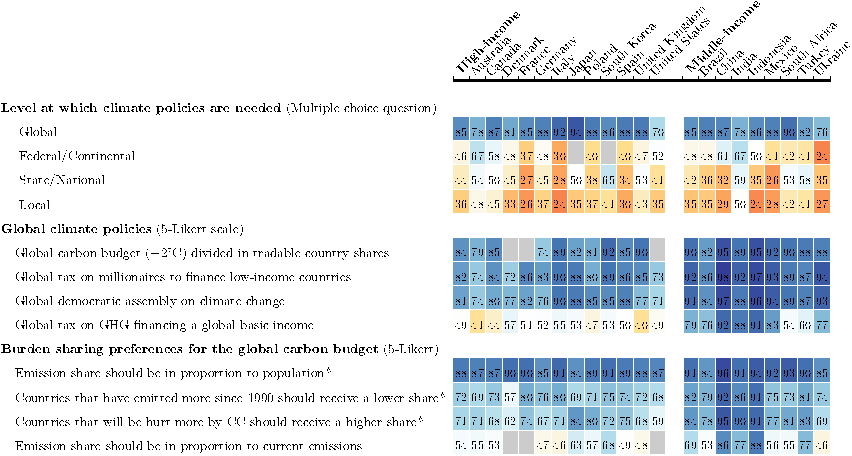
\includegraphics[height=.9\textheight]{../figures/OECD/Heatplot_global_tax_attitudes_share.pdf} % burden_share_all_share_countries
		\end{figure}
\end{frame}

\begin{frame}{The \textit{Global Climate Scheme} (GCS)\label{GCS_def}}
\bbvs \ip Our main policy of interest is the GCS, a \rose{global emissions trading system funding a global basic income}:
\bbvs \ip \small{ At the Paris agreement in 2015, all countries have agreed to contain global warming ``well below +2 $\mathrm{{}^\circ}$C''. To limit global warming to this level,~\textbf{there is a maximum amount of greenhouse gases we can emit globally}.\\ \quad \\
To meet the climate target, a limited number of permits to emit greenhouse gases can be created globally. Polluting firms would be required to buy permits to cover their emissions. Such a policy would~\textbf{make fossil fuel companies pay}~for their emissions and progressively raise the price of fossil fuels.~\textbf{Higher prices would encourage people and companies to use less fossil fuels, reducing greenhouse gas emissions.}\\ \quad \\
In accordance with the principle that each human has an equal right to pollute, the revenues generated by the sale of permits could finance a global basic income.~\textbf{Each adult in the world would receive \$30/month}, thereby lifting out of extreme poverty the 700 million people who earn less than \$2/day.\\ 
\textbf{The typical [American] would lose out financially [\$85] per month}~(as he or she would face [\$115] per month in price increases, which is higher than the \$30 they would receive). \\ \quad \\
The policy could be put in place as soon as countries totaling more than 60\% of global emissions agree on it. Countries that would refuse to take part in the policy could face sanctions (like tariffs) from the rest of the World and would be excluded from the basic income.}
\ee
\ee
\end{frame}

\begin{frame}{Net gains from the Global Climate Scheme\label{GCS_gain}}
    \begin{figure}
        \centering % TODO add map with opt out in appendix
        %\caption{  %\hyperlink{}{\beamergotobutton{See more}}
        % }
        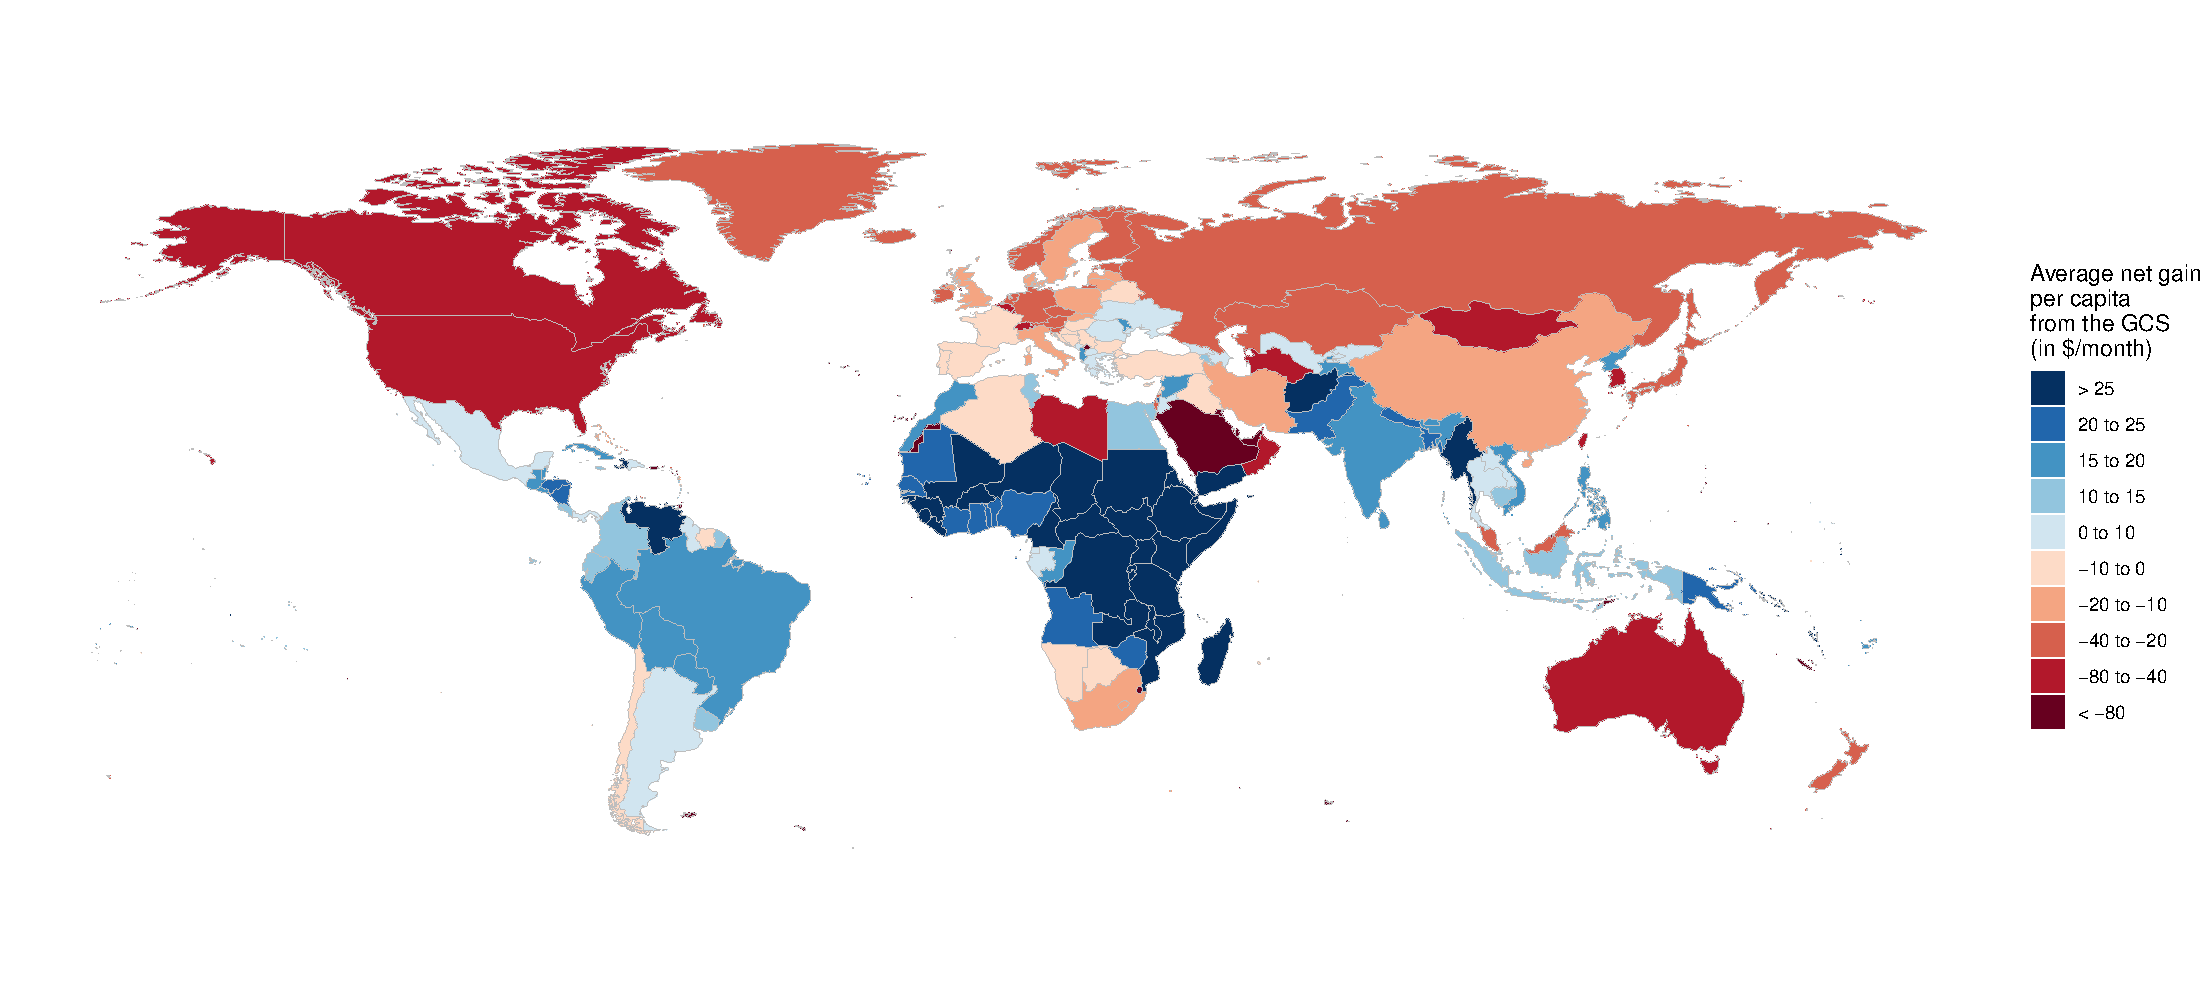
\includegraphics[height=.9\textheight]{../figures/maps/mean_gain_2030.pdf} 
    \end{figure}
\end{frame}

\begin{frame}{Support for the Global Climate Scheme\label{gcs_support}}
\bbvsp \ip To offset the losses of the median emitter, we design a \rose{National Redistribution Scheme} (NR) funded by increased income taxes on the top 5\% (US) / 1\% (Eu).
\ip We test understanding of the distributive effects of the GCS, NR, and both combined (and then give the expected answer) in an incentivized way after each policy description. \hyperlink{understanding}{\beamergotobutton{Understanding}}
\ip We also describe a national climate policy. US: Coal exit / Eu: Insulation plan (mandatory, subsidised).
\ee \vspace{-.3cm}
    \begin{figure}
        \centering % TODO perceptions G
        \only<1-3>{
\includegraphics[height=.55\textheight]{../figures/blank}}
        \only<4>{\caption{Do you support...? \textit{Yes/No} (Percentage of \textit{Yes}) \hyperlink{gcs_perceptions}{\beamergotobutton{Perceptions}} \hyperlink{conjoint_ab}{\beamergotobutton{Complementary policies}} \hyperlink{gcs_vote}{\beamergotobutton{By vote}} \hyperlink{national_policies}{\beamergotobutton{National policies}}}
        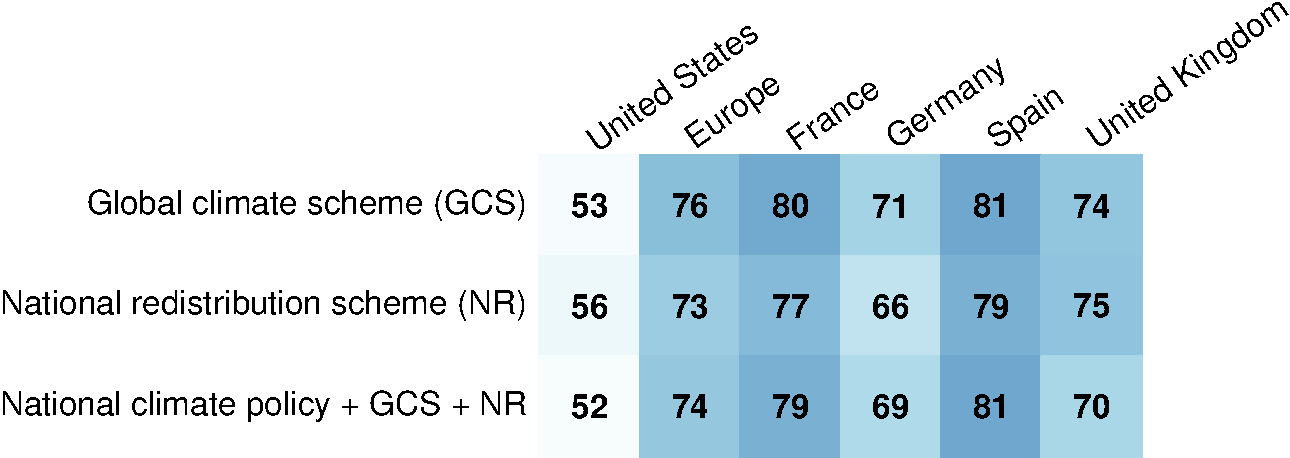
\includegraphics[height=.55\textheight]{../figures/country_comparison/support_binary_positive.pdf} } % 45
    \end{figure}
\end{frame}

\subsection{Support for other global policies}

\begin{frame}{Support for other global policies\label{other_policies}  \hyperlink{foreign_aid_conditions}{\beamergotobutton{Foreign aid}}}
	\vspace{-.3cm}
    \begin{figure}
        \centering 
        \caption{Do you support or oppose...? \textit{5-Likert scake} (Percentage of \textit{Support} among non-\textit{Indifferent})}
        \vspace{-.2cm}
        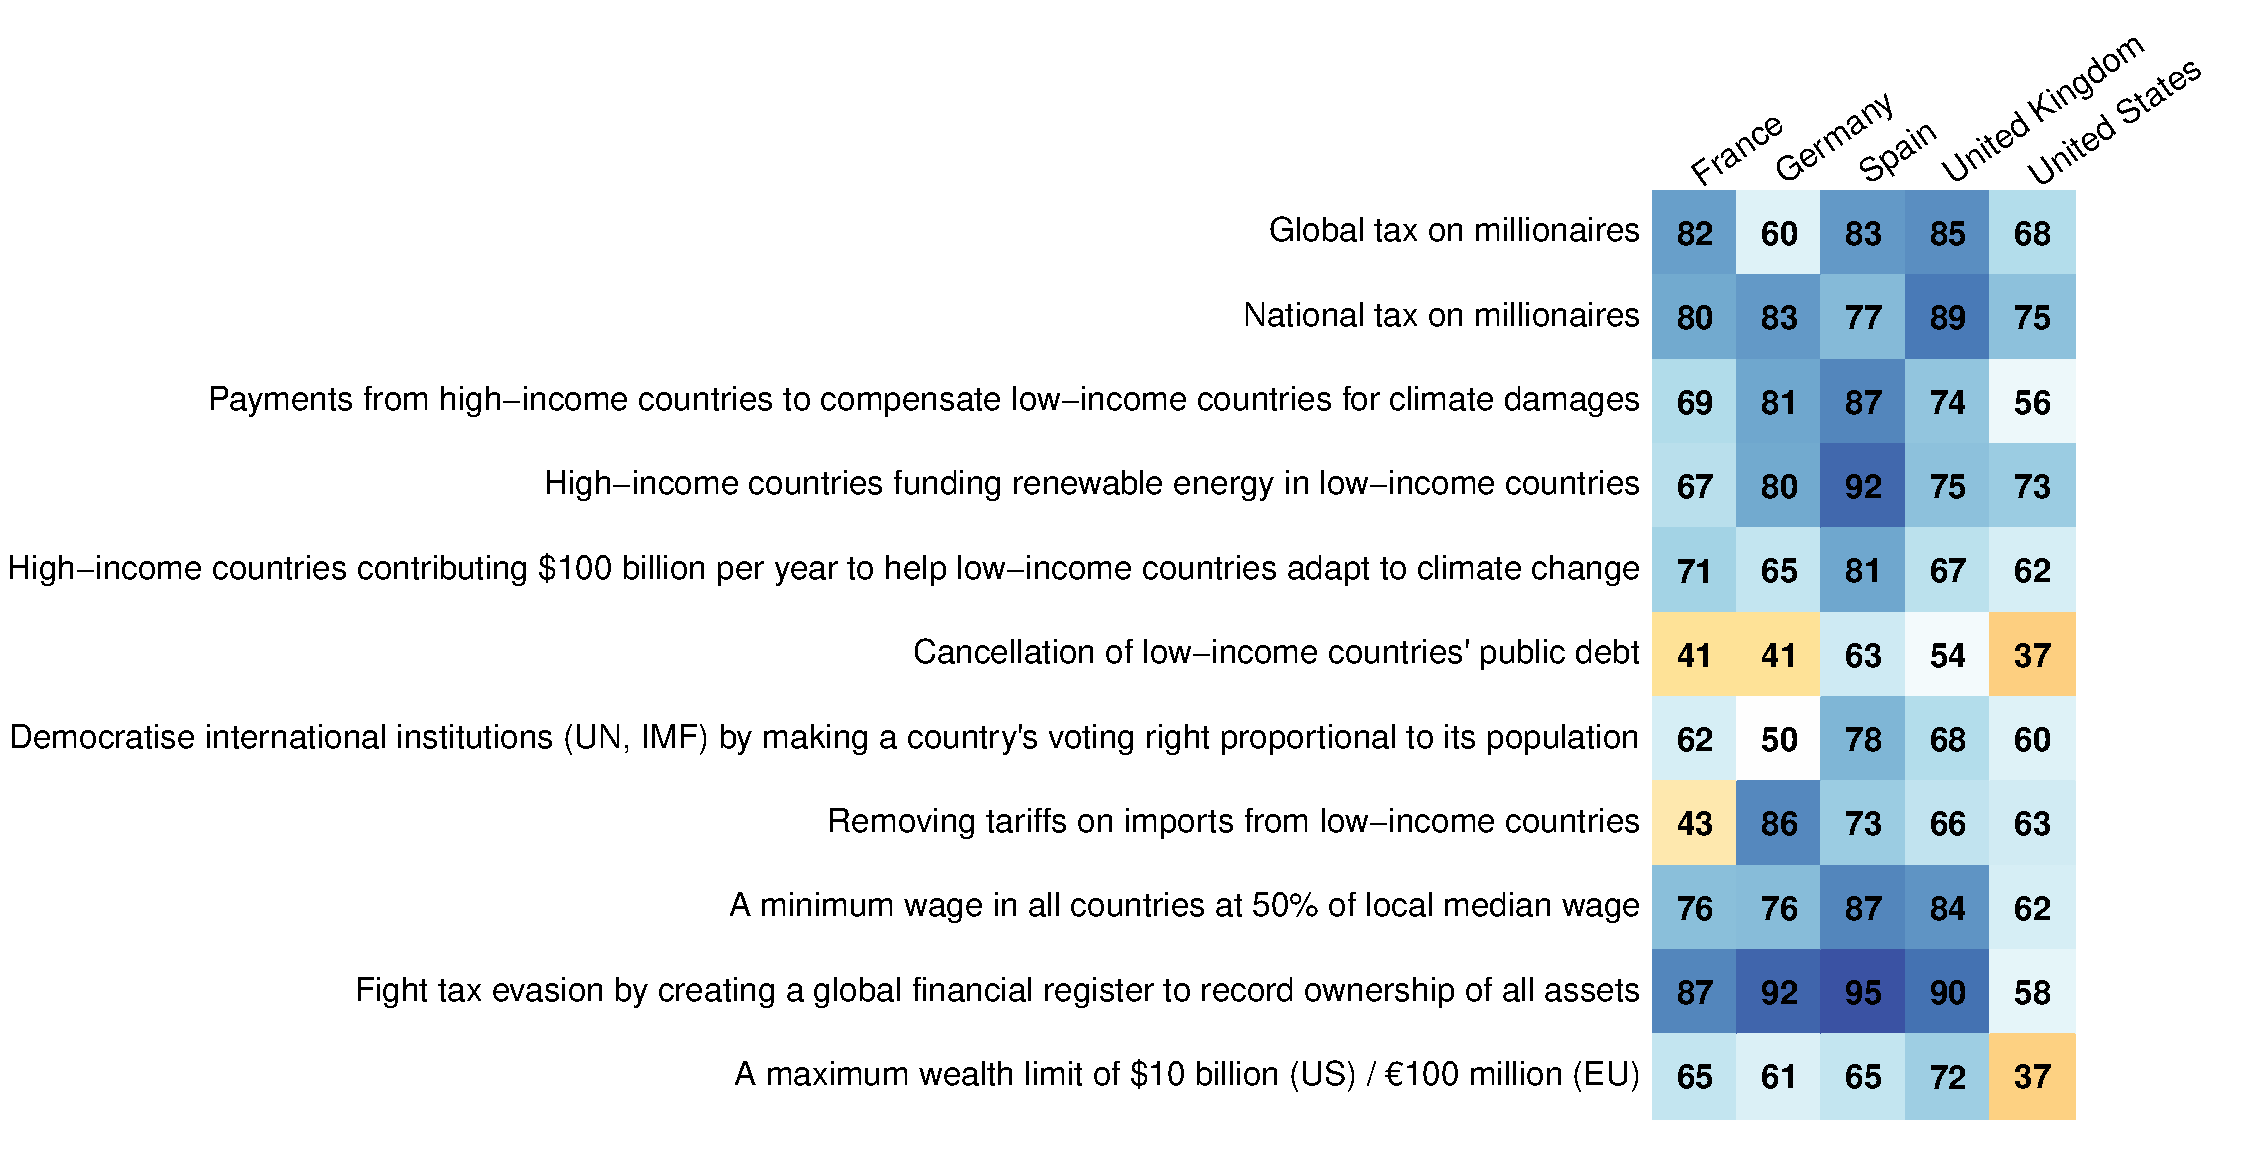
\includegraphics[height=.9\textheight]{../figures/country_comparison/support_likert_share.pdf} 
    \end{figure}
\end{frame}

\begin{frame}{Support for a global wealth tax\label{wealth_tax}  \hyperlink{foreign_aid_conditions}{\beamergotobutton{Foreign aid}}}
\bbvs \ip We describe a global tax on wealth in excess of \$/\euro{}/£ 5 million and either ask:\pause
\ee
\vspace{-.4cm}
\begin{figure}
    \centering 
    \caption{Percent of wealth tax that should go to low-income countries (\textit{mean}):}\vspace{-.2cm}% 90% give a positive amount
    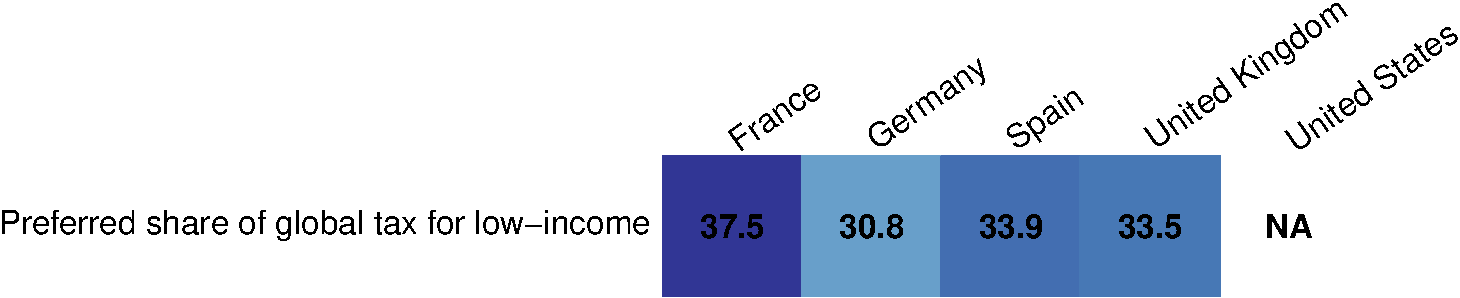
\includegraphics[height=.3\textheight]{../figures/country_comparison/global_tax_global_share_mean.pdf} 
\end{figure}\pause
    \begin{figure}
        \centering 
        \caption{Whether half of the tax revenues should go to low-income countries (vs. none).}\vspace{-.2cm}
        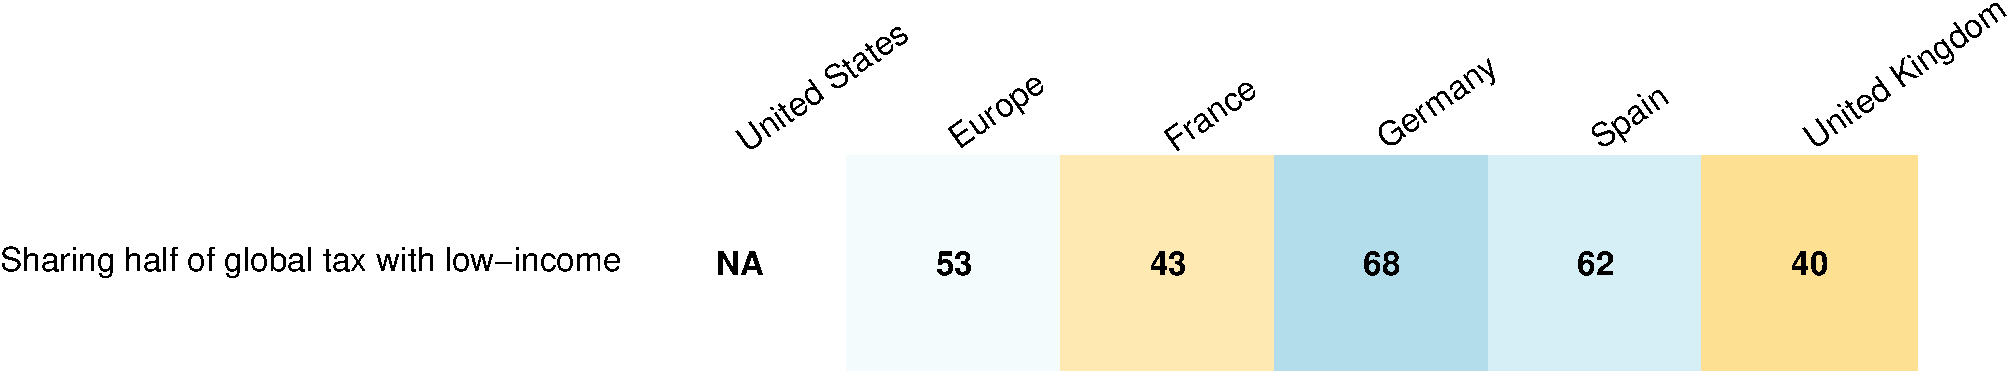
\includegraphics[height=.3\textheight]{../figures/country_comparison/global_tax_sharing_positive.pdf} 
    \end{figure}
% $\Rightarrow$ \rose{Median Eu preference is 30\% of global wealth tax for low-income countries}.
\end{frame}

\subsection{Sincerity of the support for the GCS}

% TODO appendix
% \begin{frame}{Perceptions of the Global Climate Scheme\label{}}
% 	\vspace{-.3cm}
%     \begin{figure}
%         \centering 
%         \caption{When determining your support or opposition to the Global climate scheme, which points are important to you?}
%         \vspace{-.2cm}
%         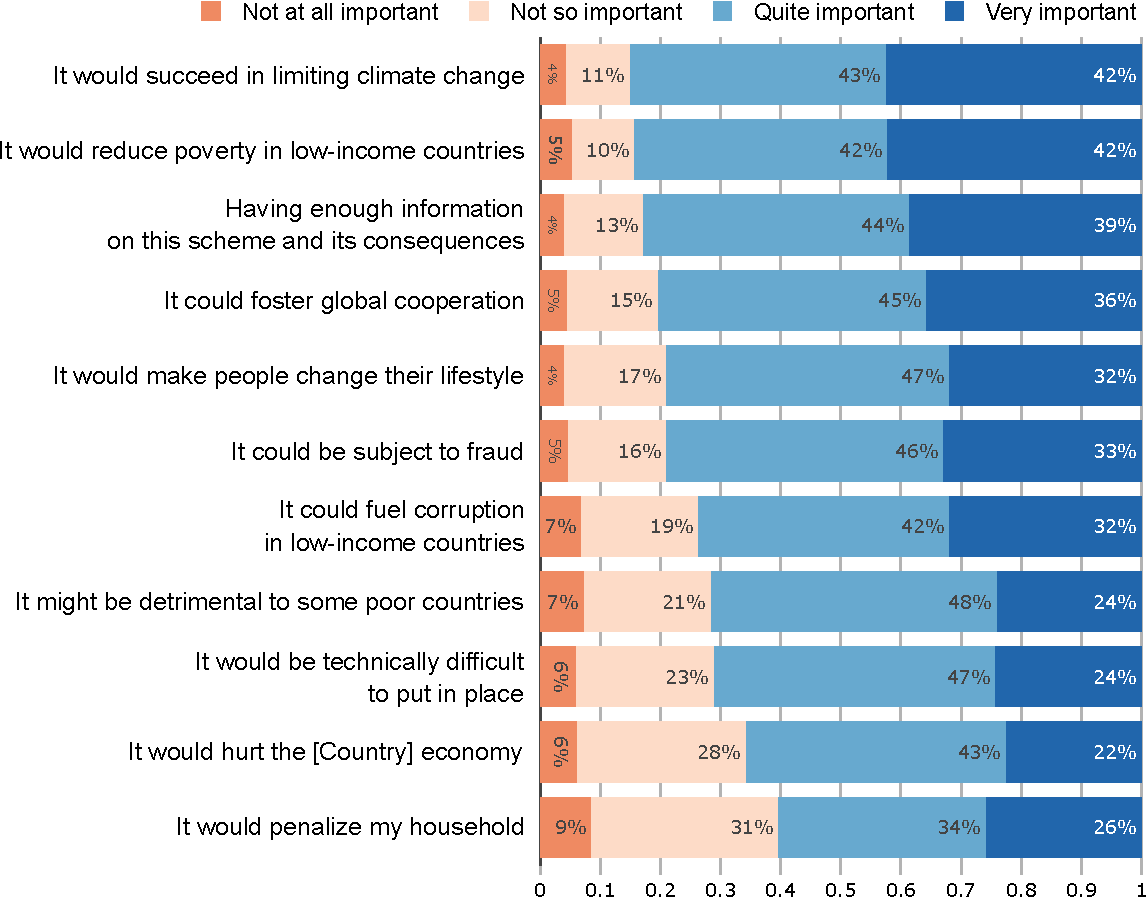
\includegraphics[height=.9\textheight]{../figures/all/gcs_important.pdf} 
%     \end{figure}
% \end{frame}

\begin{frame}{Petition\label{}}
    \begin{figure}
        \centering 
        \caption{Would you be willing to sign a petition for the [GCS / NR]? \\As soon as the survey is complete, we will send the results to the [head of state] (...) \textit{Yes/No} % U.S. President's office %, informing him what share of American people are willing to endorse the Global climate scheme. (You will NOT be asked to sign, only your answer here is required and remains anonymous.)
        }
        \vspace{-.2cm}
        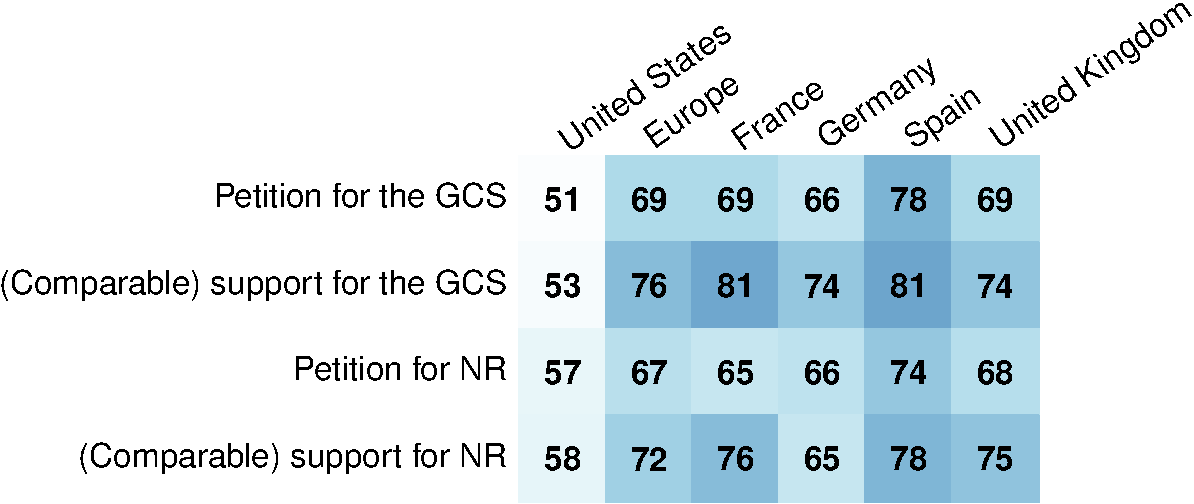
\includegraphics[height=.6\textheight]{../figures/country_comparison/petition_comparable_positive.pdf} 
    \end{figure}
	\bbvs \ip Willingness to sign a real-stake petition is generally (1 to 7 p.p.) lower than stated support.
	\ip But this is not specific to GCS, and majorities are still willing to sign the petition.
    \ee
\end{frame}

\begin{frame}{List experiment\label{}}
    \vspace*{-.1cm}
\bbvs \ip We ask \textit{Among the policies below, how many do you support?}, randomly varying the list of policies.
\ip The difference in mean number of supported policies for lists with and without the GCS should equal the support for GCS. \blue{If} the \rose{tacit support} \blue{is lower}, it may indicate a \blue{social desirability bias}. \pause
\ee
{\footnotesize
    \begin{table}[h]\label{tab:list_exp}\vspace*{-.35cm}
        %\caption{Number of supported policies in the list experiment in function of the composition of the list. } % Beware, this question is quite unusual. \\ Among the policies below, how many do you support?  \\ Coal exit, Marriage only for opposite-sex couples 
        \makebox[\textwidth][c]{
\begin{tabular}{@{\extracolsep{5pt}}lccc} 
\\[-1.8ex]\hline 
\hline \\[-1.8ex] 
 & \multicolumn{3}{c}{Number of supported policies} \\ 
\cline{2-4} 
\\[-1.8ex] & All & US & Europe \\ 
\hline \\[-1.8ex] 
 List contains: GCS & 0.624$^{***}$ & 0.524$^{***}$ & 0.724$^{***}$ \\ 
  & (0.028) & (0.041) & (0.036) \\ 
\hline  \\[-1.8ex] \textit{Support for GCS} & 0.65  &  0.542  &  0.757 \\
\textit{Social desirability bias} & \textit{$ -0.026 $} & \textit{$ -0.018 $} & \textit{$ -0.033 $}\\
\textit{80\% C.I. for the bias} & \textit{ $[ -0.06 ; 0.01 ]$ } & \textit{ $[ -0.07 ; 0.01 ]$} & \textit{ $[ -0.08 ; 0.01 ]$}\\
 \hline \\[-1.8ex] 
Constant & 1.317 & 1.147 & 1.486 \\ 
Observations & 6,000 & 3,000 & 3,000 \\ 
R$^{2}$ & 0.089 & 0.065 & 0.125 \\ 
\hline 
\hline \\[-1.8ex] 
\textit{Note:}  & \multicolumn{3}{r}{$^{*}$p$<$0.1; $^{**}$p$<$0.05; $^{***}$p$<$0.01} \\ 
\end{tabular} }
      \end{table}
}
$\Rightarrow$ \blue{No (significant) social desirability bias.} 
%\blue{Small social desirability bias for GCS and NR in the U.S.} (tacit support is 5 p.p.*** lower), \blue{none in Europe}. 
\end{frame}

% TODO appendix
% \begin{frame}{Conjoint analyses: interaction with other policies\label{}} 
%     \bbvs \ip National climate policy (C) is as supported as the GCS, but no substitute for it.
% 	\ip Support for the GCS does not increase when complemented by National Redistribution.
% 	\ip $\Rightarrow$ Confirms that the \rose{monetary loss is not a primary concern} for one's attitude toward the GCS.
%     \ee
%     \begin{figure} \vspace*{-.5cm}
%         \centering 
%         \caption{Among the two following bundles of policies, which one would you prefer?}
%         \vspace{-.2cm} 
%         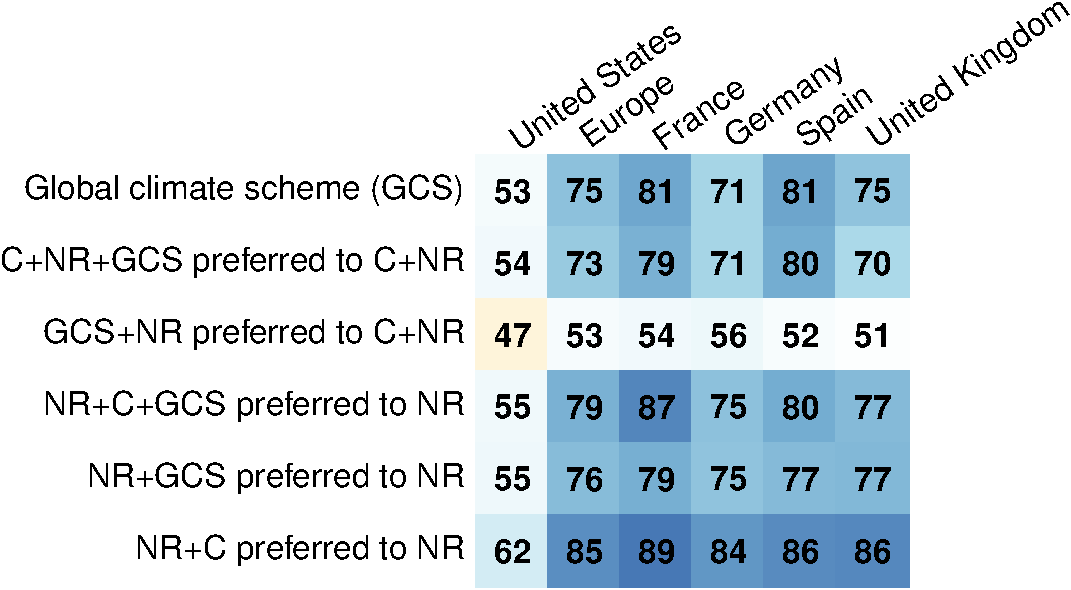
\includegraphics[height=.65\textheight]{../figures/country_comparison/conjoint_ab_positive.pdf} 
%     \end{figure}
% \end{frame}

\begin{frame}{Conjoint analyses: influence on electoral prospects\label{conjoint_c}} 
    % \begin{figure}
    %     \centering 
    %     \caption{Imagine if the [Democratic and Republican presidential candidates in 2024] campaigned with the following policies in their platforms. \\
	% 	Which of these candidates would you vote for? \\
	% 	~[FR: second round of presidential; DE, ES, UK: two favorite candidates in one's constituency]}
    %     \vspace{-.2cm} 
    %     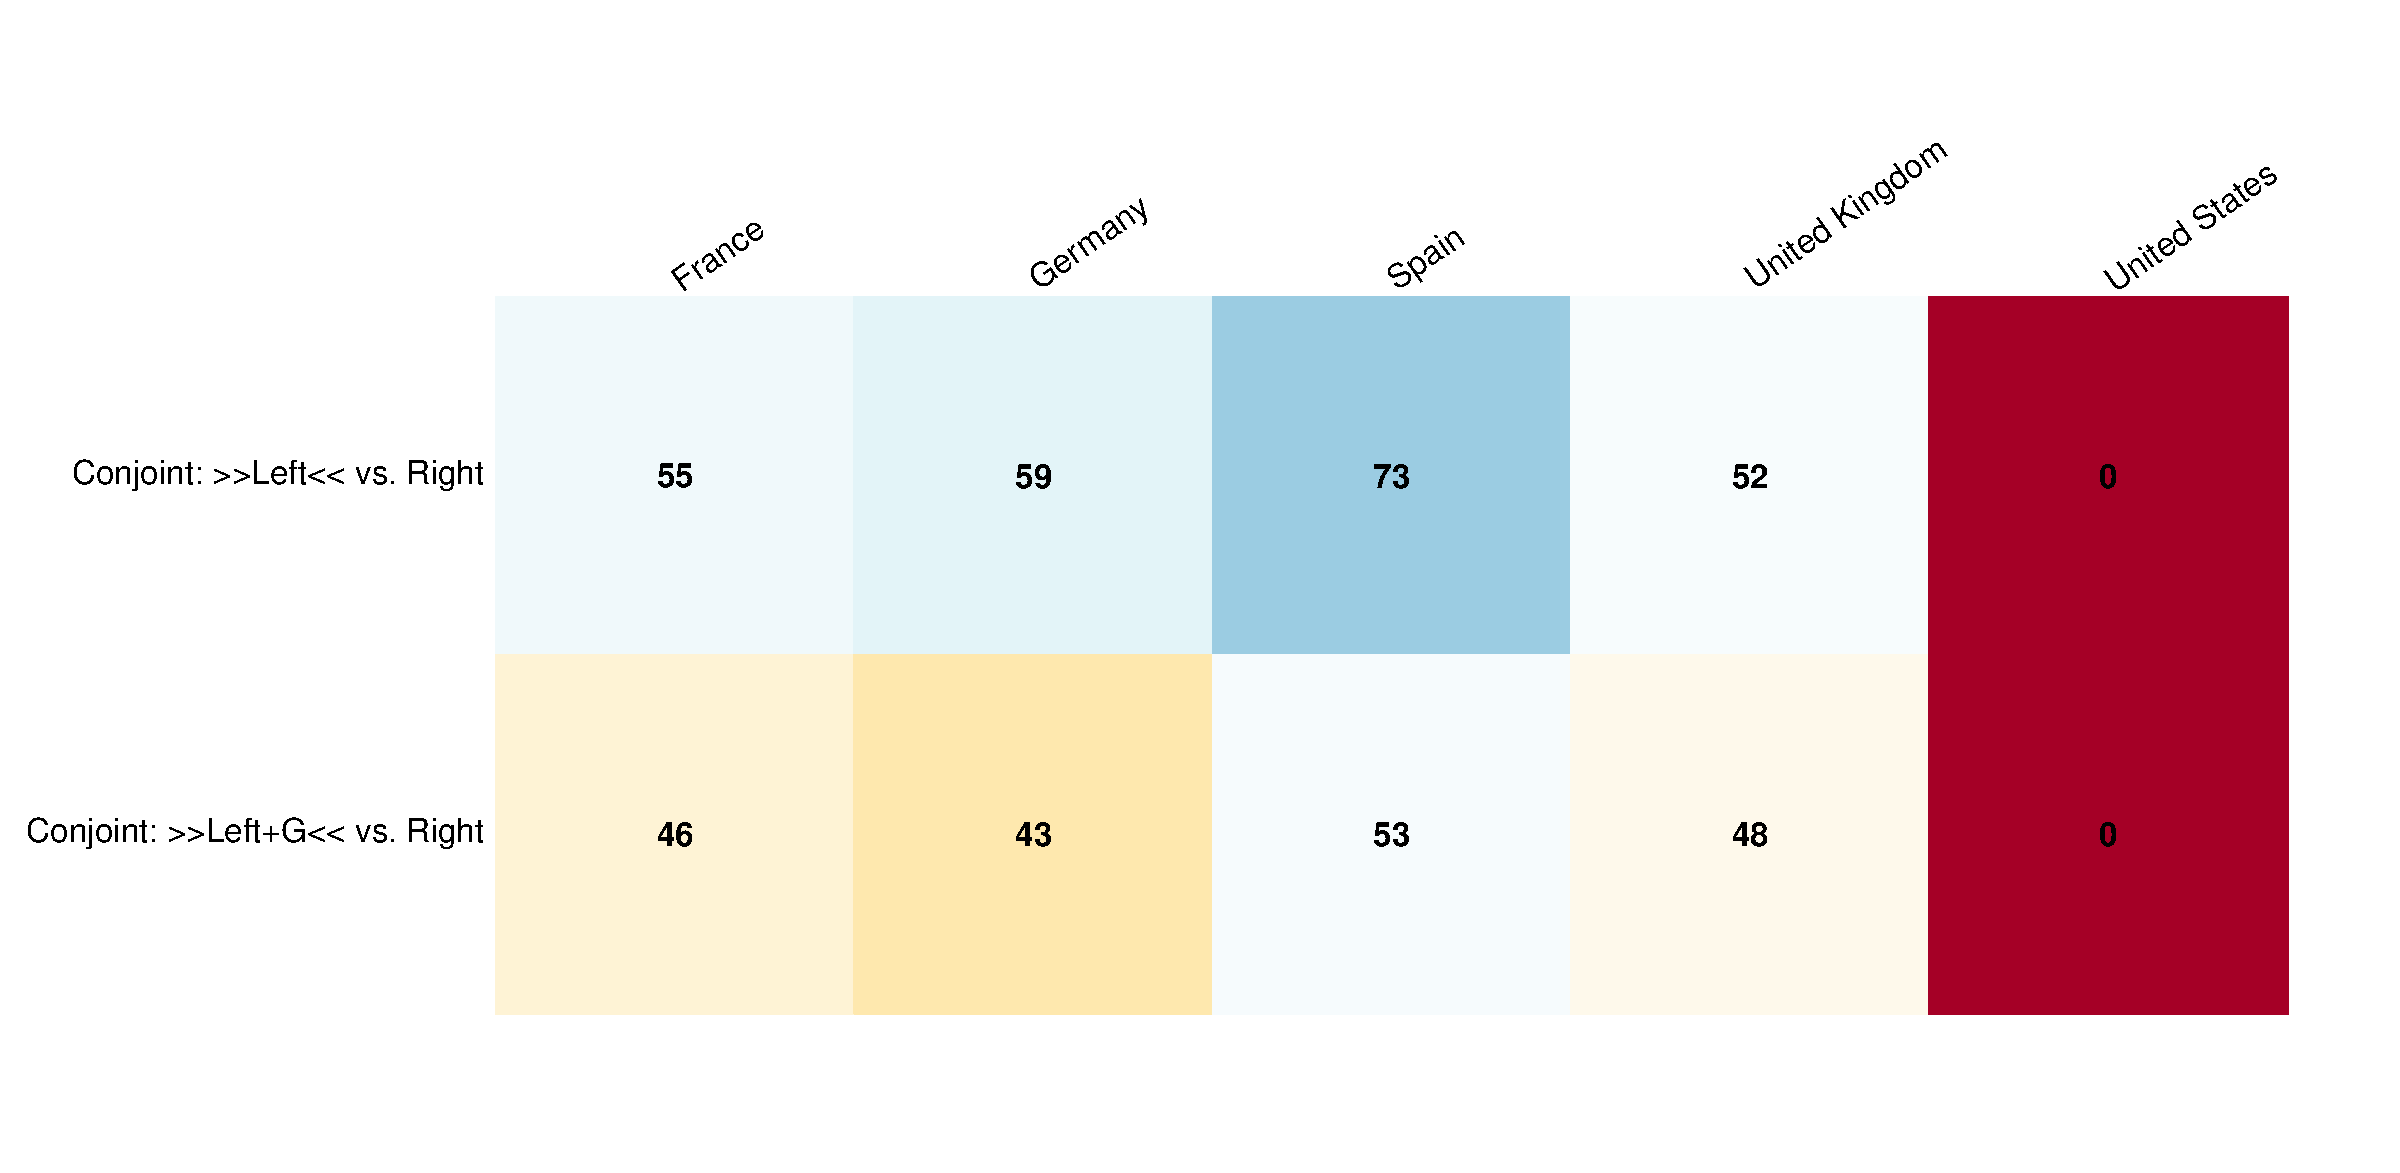
\includegraphics[height=.5\textheight]{../figures/country_comparison/conjoint_c_positive.pdf} % /all/ca_r.png + in US: only on non-Republican
    % \end{figure}
    % {\footnotesize
    \only<1>{
        \begin{center}Choice between a conservative platform and a progressive platform with/without the GCS.\end{center}
    \begin{columns}
        \begin{column}{0.5\textwidth}
            \begin{figure}
                \centering 
                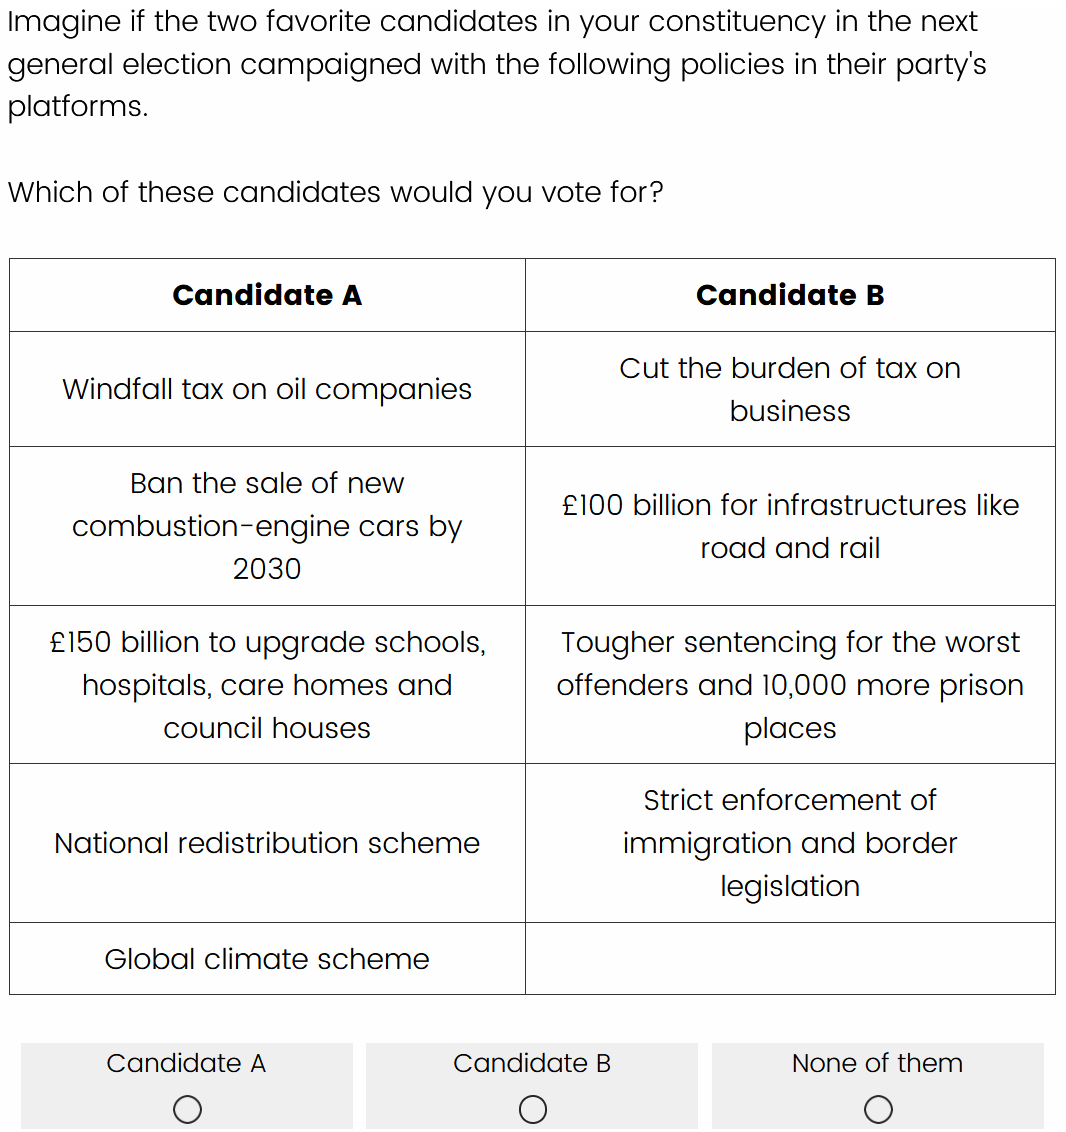
\includegraphics[height=.8\textheight]{../figures/UK/screenshot_en_with}
            \end{figure}
        \end{column}
        \begin{column}{0.5\textwidth}
            \begin{figure}
                \centering 
                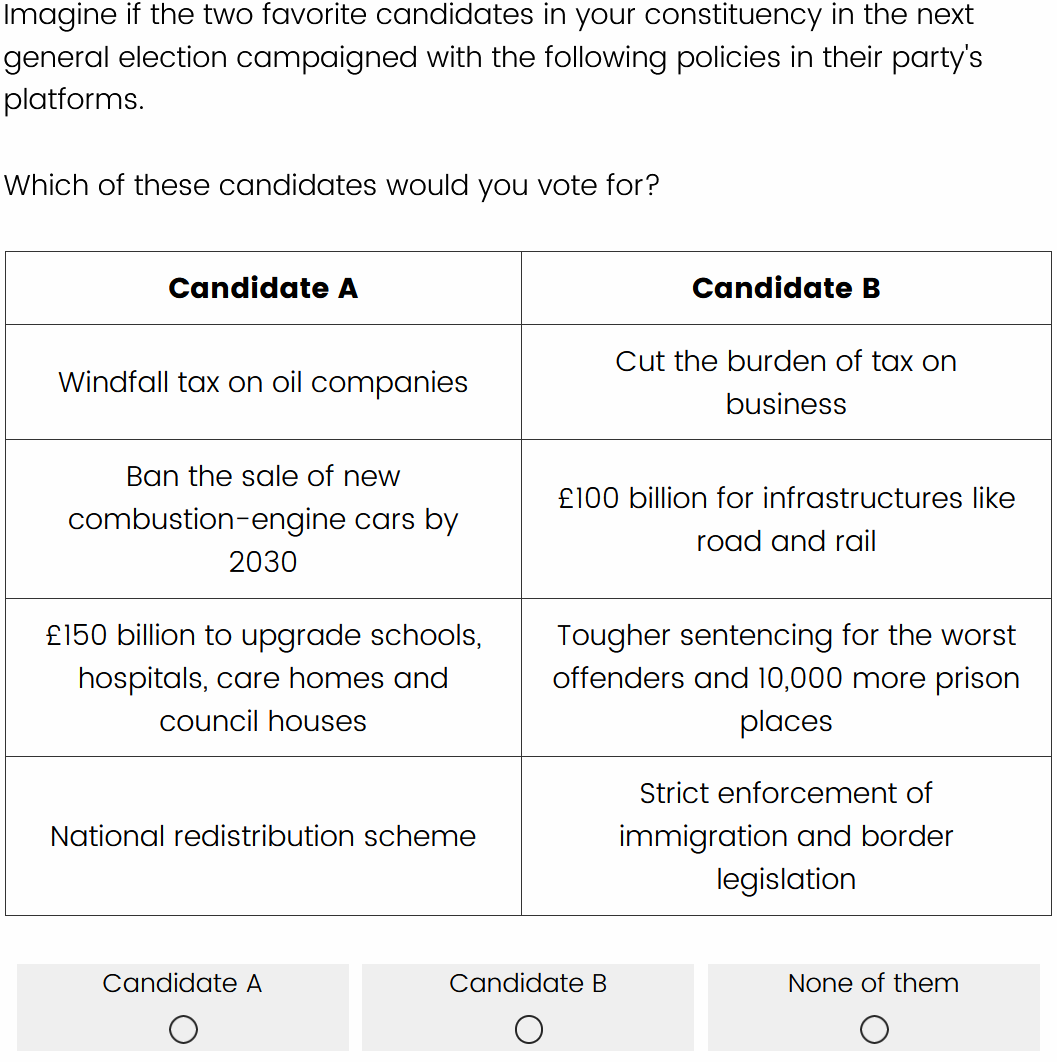
\includegraphics[height=.8\textheight]{../figures/UK/screenshot_en_wo}
            \end{figure}
        \end{column}
    \end{columns}
    }
    \only<2->{
    \begin{table}[h]\label{tab:conjoint_c_wo_none}\vspace*{-.2cm}
        \caption{Imagine if the [Democratic and Republican presidential candidates in 2024] campaigned with the following policies in their platforms. [Credible Progressive and Conservative platforms] \\ % TODO See More
        Which of these candidates would you vote for? \textit{A; B; None of them} \\
        ~[FR: second round of presidential; DE, ES, UK: two favorite candidates in one's constituency]} % Beware, this question is quite unusual. \\ Among the policies below, how many do you support?  \\ Coal exit, Marriage only for opposite-sex couples 
        \makebox[\textwidth][c]{
\begin{tabular}{@{\extracolsep{5pt}}lcccccc} 
\\[-1.8ex]\hline 
\hline \\[-1.8ex] 
 & \multicolumn{6}{c}{Prefers the Progressive platform} \\ 
\cline{2-7} 
\\[-1.8ex] & All & United States & France & Germany & UK & Spain \\ 
\hline \\[-1.8ex] 
 GCS in Progressive platform & 0.028$^{*}$ & 0.029 & 0.112$^{***}$ & 0.015 & 0.008 & $-$0.015 \\ 
  & (0.014) & (0.022) & (0.041) & (0.033) & (0.040) & (0.038) \\ 
 \hline \\[-1.8ex] 
Constant & 0.623 & 0.604 & 0.55 & 0.7 & 0.551 & 0.775 \\ 
Observations & 5,202 & 2,619 & 605 & 813 & 661 & 504 \\ 
R$^{2}$ & 0.001 & 0.001 & 0.013 & 0.0003 & 0.0001 & 0.0003 \\ 
\hline 
\hline \\[-1.8ex] 
\end{tabular} 
}
        {\footnotesize \textit{Note:} The 14\% of \textit{None} answers have been excluded from the regression samples. GCS has no significant influence on them. }
      \end{table} \vspace*{-.2cm}
      \bbvs \ip \rose{A progressive candidate would not lose votes by endorsing the GCS}, and could even gain 11 p.p.*** in France.
      \ee
      }
% }
\end{frame}

\begin{frame}{Conjoint analyses: influence on preferred platform\label{conjoint_d}} 
    \bbvs \ip We ask the preference between two progressive platforms, where each measure is taken at random. \\ The GCS is included in one of the platforms.
    \ee
    \begin{figure} \vspace*{-.3cm}
        \centering 
        \caption{Imagine that a [Left or Center-left coalition wins the next elections]. Here are two possible platforms on which [the coalition] may campaign (the policies in each platform are randomly drawn from a pool of credible [Left/Center-left] policies).
		\\ Even if you do not support the Left, which of these platforms do you prefer? 
		\\ ~[FR: Left or center-left; DE: rot-rot-grüne; ES: PSOE; UK: Labour; US: Democratic primary (\textit{not asked to Republican})]
		}
        \vspace{-.2cm} 
        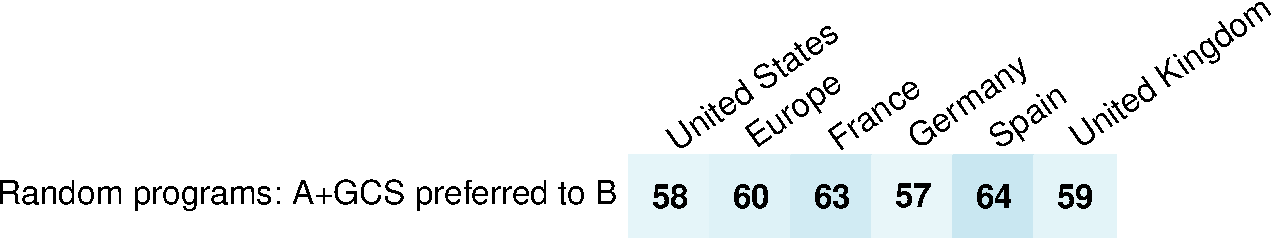
\includegraphics[width=\textwidth]{../figures/country_comparison/conjoint_left_ag_b_binary_positive.pdf} 
    \end{figure}
    $\Rightarrow$ \rose{Majorities prefer platforms that include the GCS.}
\end{frame}

% TODO appendix
% \begin{frame}{Conjoint analyses: influence on preferred platform (Eu)\label{}} 
%     \begin{figure}\vspace{-.2cm}
%         \centering 
%         \caption{%Imagine that a [Left or Center-left coalition wins the next elections]. Here are two possible platforms on which [the coalition] may campaign (the policies in each platform are randomly drawn from a pool of credible [Left/Center-left] policies).\\
% 		(...) Even if you do not support the Left, which of these platforms do you prefer? 
% 		%\\ ~[FR: Left or center-left; DE: rot-rot-grüne; ES: PSOE; UK: Labour]
% 		}
%         \vspace{-.2cm} 
%         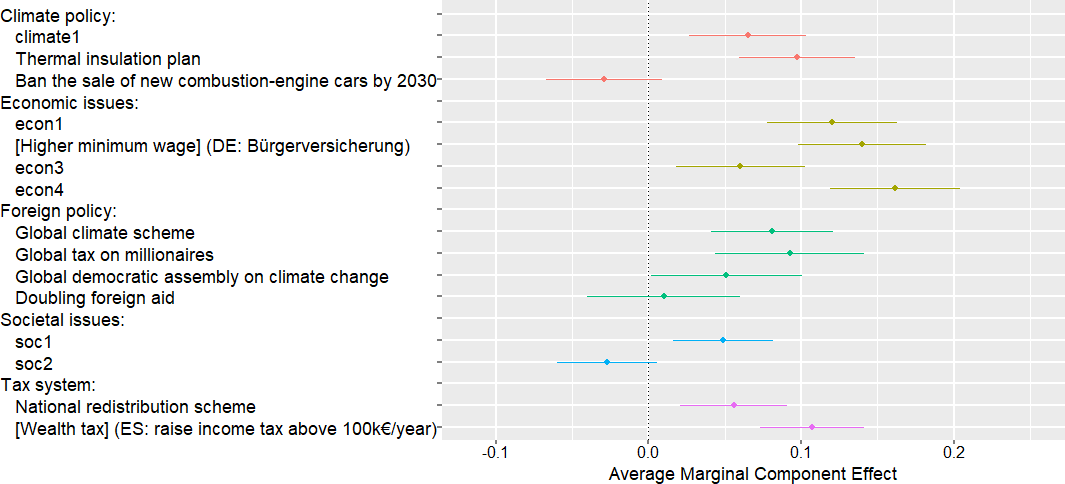
\includegraphics[height=.7\textheight]{../figures/EU/ca_r.png} 
%     \end{figure}
%     \bbvs \ip \rose{Europeans prefer platforms that include the GCS} and without the ban on thermal cars (a planned policy).
% 	\ip The effect of GCS is among the highest (wealth tax, better public services, higher minimum wage).
%     \ee
% \end{frame}

\begin{frame}{Conjoint analyses: influence on preferred platform (UK)\label{conjoint_r_uk} \hyperlink{conjoint_r_eu}{\beamergotobutton{EU}} \hyperlink{conjoint_r_fr}{\beamergotobutton{FR}} \hyperlink{conjoint_r_us}{\beamergotobutton{U.S.}}} 
	%\vspace{-.2cm}
    % \bbvs \ip France shows that there can be a \rose{mismatch between preferred} policies (insulation plan, public services, global tax, GCS) \rose{and enacted policies} (higher retirement age and ban on thermal cars: the least preferred). \ee
    \begin{figure}\vspace{-.2cm}
        \centering 
        \caption{Imagine that the Labour wins the next elections. Here are two possible platforms on which it may campaign (the policies in each platform are randomly drawn from a pool of credible Labour policies).\\
		(...) %Even if you do not support the Left, 
        which of these platforms do you prefer? %(les mesures de ces programmes sont tirés aléatoirement depuis un ensemble de mesures de gauche ou centre gauche).
		%\\ Même si vous n'êtes pas de gauche ou centre gauche		, lequel de ces programmes préférez-vous ?
        }
        \vspace{-.2cm} 
        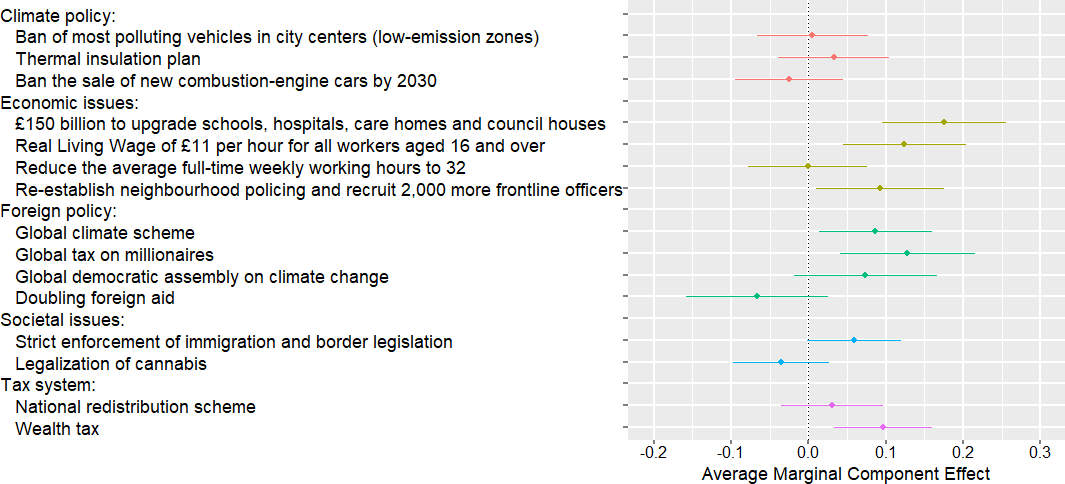
\includegraphics[height=.77\textheight]{../figures/UK/ca_r.png} 
    \end{figure}
\end{frame}

% TODO appendix
% \begin{frame}{Conjoint analyses: influence on preferred platform (US)\label{}} 
%     \bbvs \ip \rose{Endorsing the GCS is not determinant to gain the Democratic primary.}
%     \ee
%     \begin{figure}\vspace{-.4cm}
%         \centering 
%         \caption{[Only on non-Republican] Imagine that at the 2024 Democratic party presidential primaries, the two main candidates campaign with the following key policies in their platforms.\\
% 		Which of these candidates do you prefer?}
%         \vspace{-.2cm} 
%         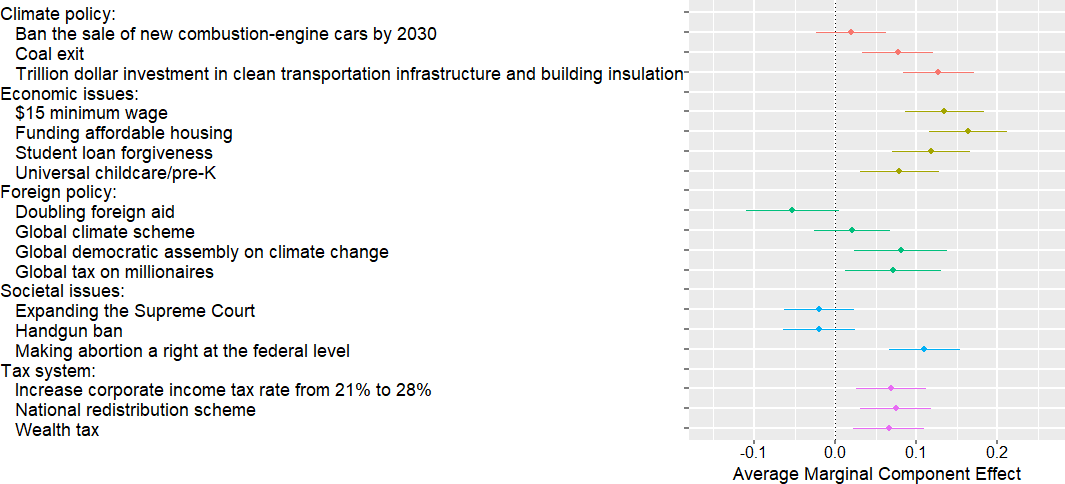
\includegraphics[height=.7\textheight]{../figures/US1/ca_r.png} 
%     \end{figure}
% \end{frame}

% \begin{frame}{Prioritization\label{}}
%     \begin{columns}
%         \begin{column}{0.35\textwidth}\vspace{-1cm}
%             \bbvs \ip %``In this question, 
% 			``you have 100 points that you can allocate to different policies. The more you give points to a policy, the more you support it.\\ % TODO: highlight synchronously
%             How do you allocate the points among the following policies?'' \\~[6 policies taken at random]
%             \ip GCS is as prioritized as the average policy, or even more in France and Germany. \\ It is more prioritized than some planned climate policies, like the ban on thermal cars.
%             \ip The global tax on millionaires is among the most prioritized measures.\\ It as prioritized as a national wealth tax, if not more.
%             \ip Most prioritized are better public services and a higher minimum wage.
%             \ee       
%         \end{column}
%         \begin{column}{0.65\textwidth}\vspace{-.6cm}
%             \begin{figure}
%                 \centering 
%                 \caption{\quad ~ \quad ~ \quad Mean number of points}
%                 \vspace{-.3cm}
%                 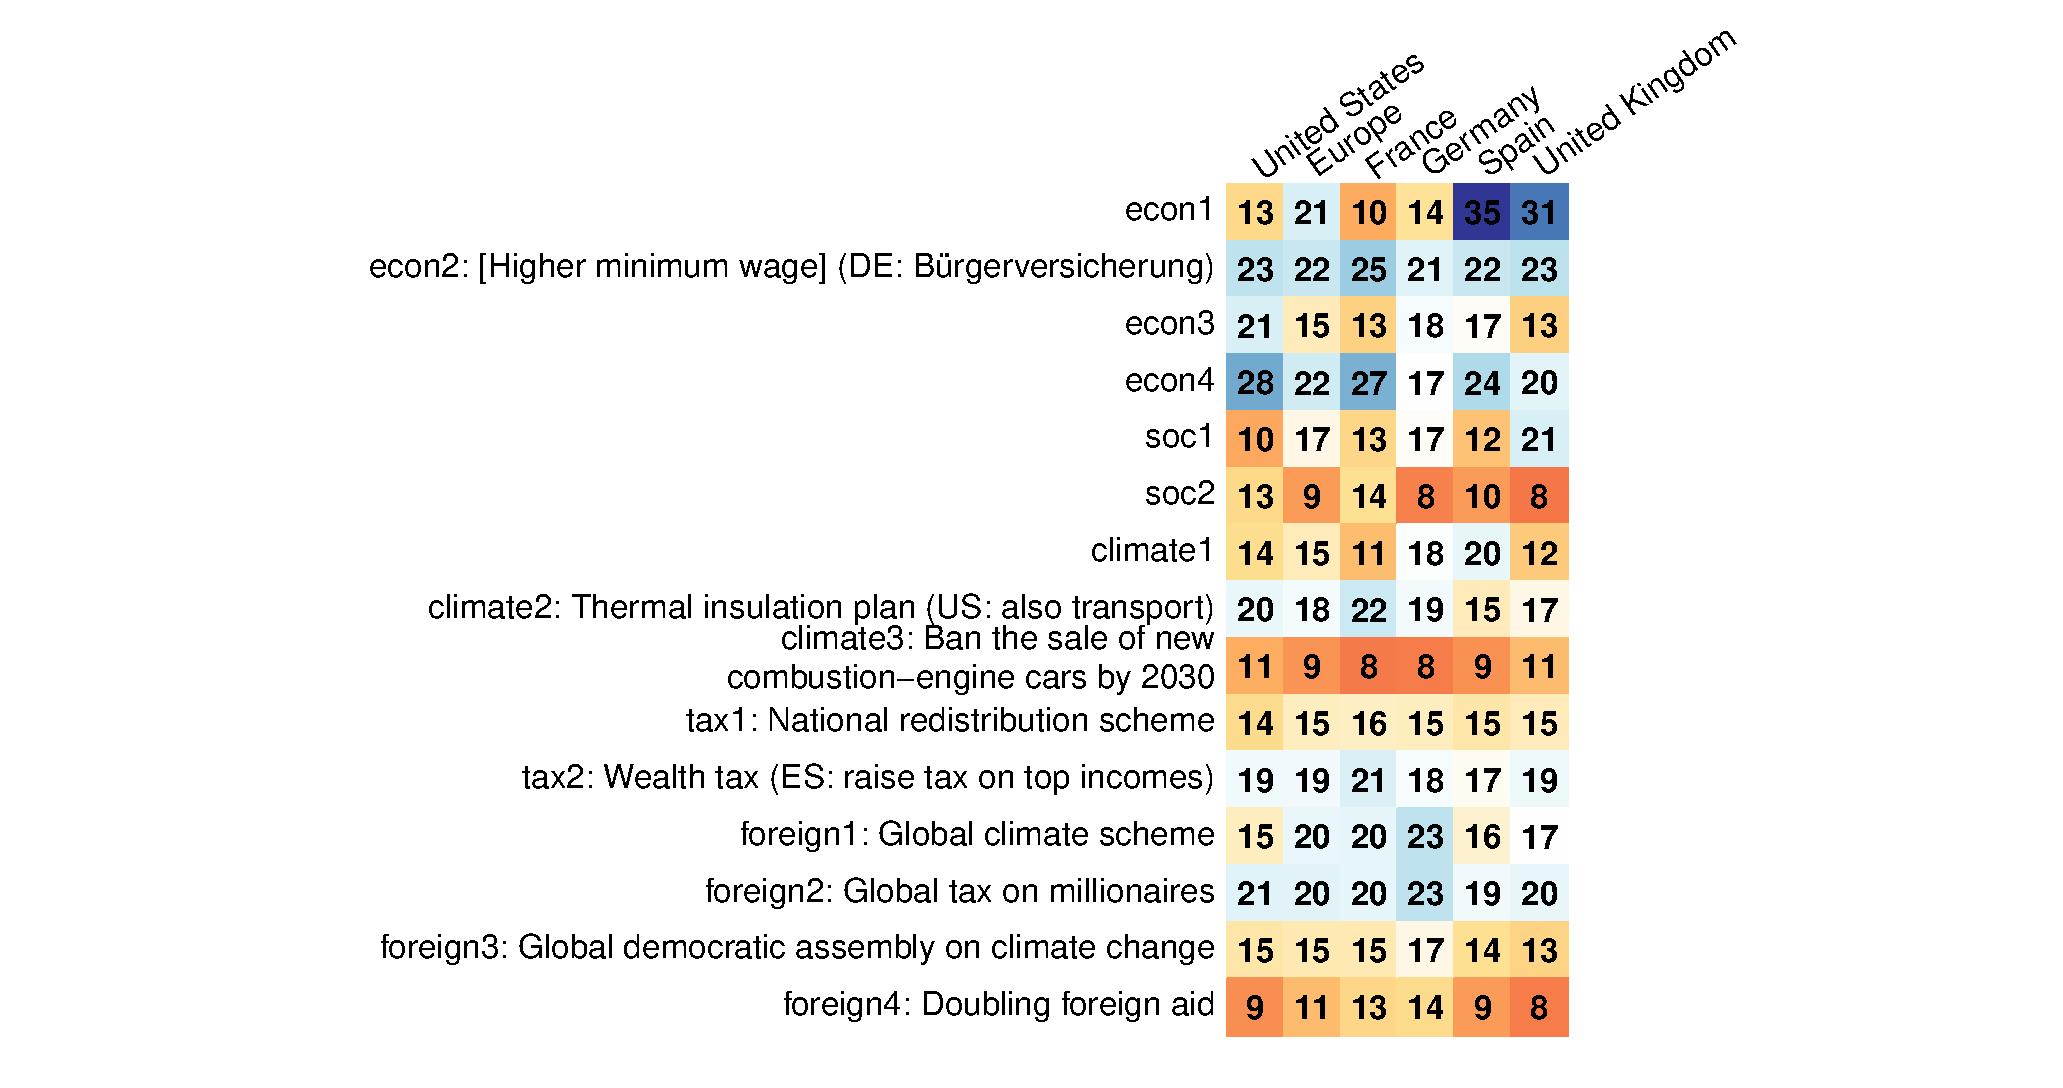
\includegraphics[width=\columnwidth]{../figures/country_comparison/points_mean.pdf} 
%             \end{figure}
%         \end{column}
%     \end{columns}
% \end{frame}

\subsection{Second-order beliefs}

\begin{frame}{Belief about the support\label{}}
	\bbvs \ip Beliefs on the support for the GCS are relatively accurate: \\ 
    \quad \blue{no evidence of pluralistic ignorance in the U.S. \\ 
    \quad an underestimation by 15-20 p.p. in Eu}.
    \ee \vspace*{-.4cm}
    \begin{figure}
        \centering 
        \caption{According to you, what percentage of [Americans] answer \textit{Yes} to the previous question? \\ The three people who are closest to the true value get [\$50].  \textit{Mean answer}
        }
        \vspace{-.2cm}
        
\includegraphics[height=.6\textheight]{../figures/country_comparison/belief_all_mean.pdf} 
    \end{figure}
\end{frame}

\subsection{Universalist values}

\begin{frame}{Donation to Africans vs. fellow citizens\label{donation}}
	\bbvs \ip Respondents might win a \$/\euro{}/£ lottery prize, they have to decide which share to donate if they win. \\ Donation is to people in need, either in Africa or in their own country (random treatment).
    \ee \pause
    \begin{table}[h]\label{tab:donation}\vspace*{-.35cm}
        \caption{(...) In case you are winner of the lottery, what share of the [\$]100 would you donate to [African / [own country]] people living in poverty through GiveDirectly?} 
        \makebox[\textwidth][c]{
\begin{tabular}{@{\extracolsep{5pt}}lccc} 
\\[-1.8ex]\hline 
\hline \\[-1.8ex] 
 & \multicolumn{3}{c}{Donation to poor people (in \%)} \\ 
\cline{2-4} 
\\[-1.8ex] & All & US & Eu \\ 
\hline \\[-1.8ex] 
 Poor is in own country & 1.080 & 3.009$^{**}$ & $-$0.903 \\ 
  & (0.968) & (1.452) & (1.277) \\ 
 \hline \\[-1.8ex] 
Mean & 33.468 & 32.948 & 33.999 \\ 
Observations & 5,235 & 2,643 & 2,592 \\ 
R$^{2}$ & 0.0003 & 0.002 & 0.0002 \\ 
\hline 
\hline \\[-1.8ex] 
\end{tabular} }
      \end{table}
      $\Rightarrow$ \blue{U.S. non-voters and Trump voters donate 5 to 6 p.p. more to fellow citizens, others give the same amount.}
      \\ Other results on universalism:  \hyperlink{prioritization}{\beamergotobutton{Prioritization}} \hyperlink{negotiation}{\beamergotobutton{Negotiations}} \hyperlink{group_defended}{\beamergotobutton{Group defended}} \hyperlink{problems}{\beamergotobutton{Global issues}}
\end{frame}

% TODO appendix
% \begin{frame}{International climate negotiations\label{}}
%     \begin{figure}
%         \centering 
%         \caption{In international climate negotiations, would you prefer [U.S.] diplomats to defend [U.S.] interests or global justice?
%         }
%         \vspace{-.2cm}
%         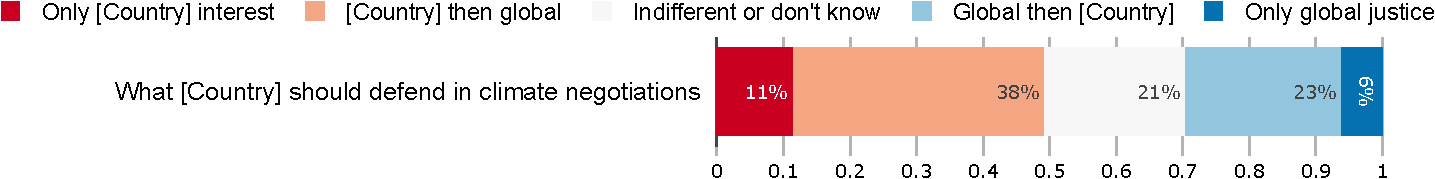
\includegraphics[width=\textwidth]{../figures/all/negotiation.pdf} 
%     \end{figure}
% 	\bbvs \ip The typical answer is to defend one's country's ``interests, to the extent it respects global justice.''
%     \ip Only one eigth wants to defend one's country's ``interests, even if it goes against global justice.''
%     \ee
% \end{frame}

% \begin{frame}{Group defended\label{}}
%     \begin{figure}
%         \centering 
%         \caption{What group do you defend when you vote?
%         }
%         \vspace{-.2cm}
%         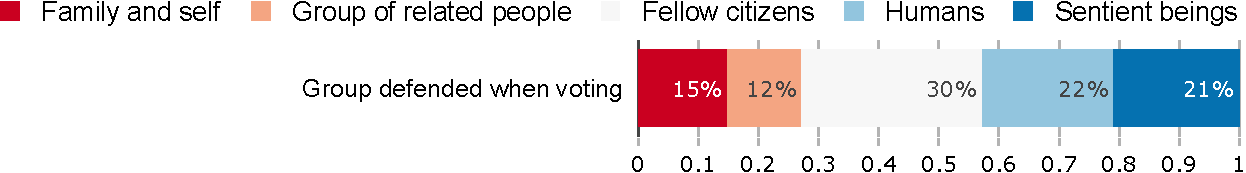
\includegraphics[width=\textwidth]{../figures/all/group_defended_agg2.pdf} 
%     \end{figure}
% 	\bbvs \ip The most defended group is one's fellow citizens.
%     \ip \blue{$~$40\% are universalist}, i.e. defend all humans or sentient beings.
%     \ee
% \end{frame}

% \begin{frame}{Biggest issues\label{}}
%     \begin{figure}
%         \centering 
%         \caption{To what extent do you think the following issues are a problem? \textit{5-Likert scale} \\(Mean of answers recoded in [-2, +2])
%         }
%         \vspace{-.2cm}
%         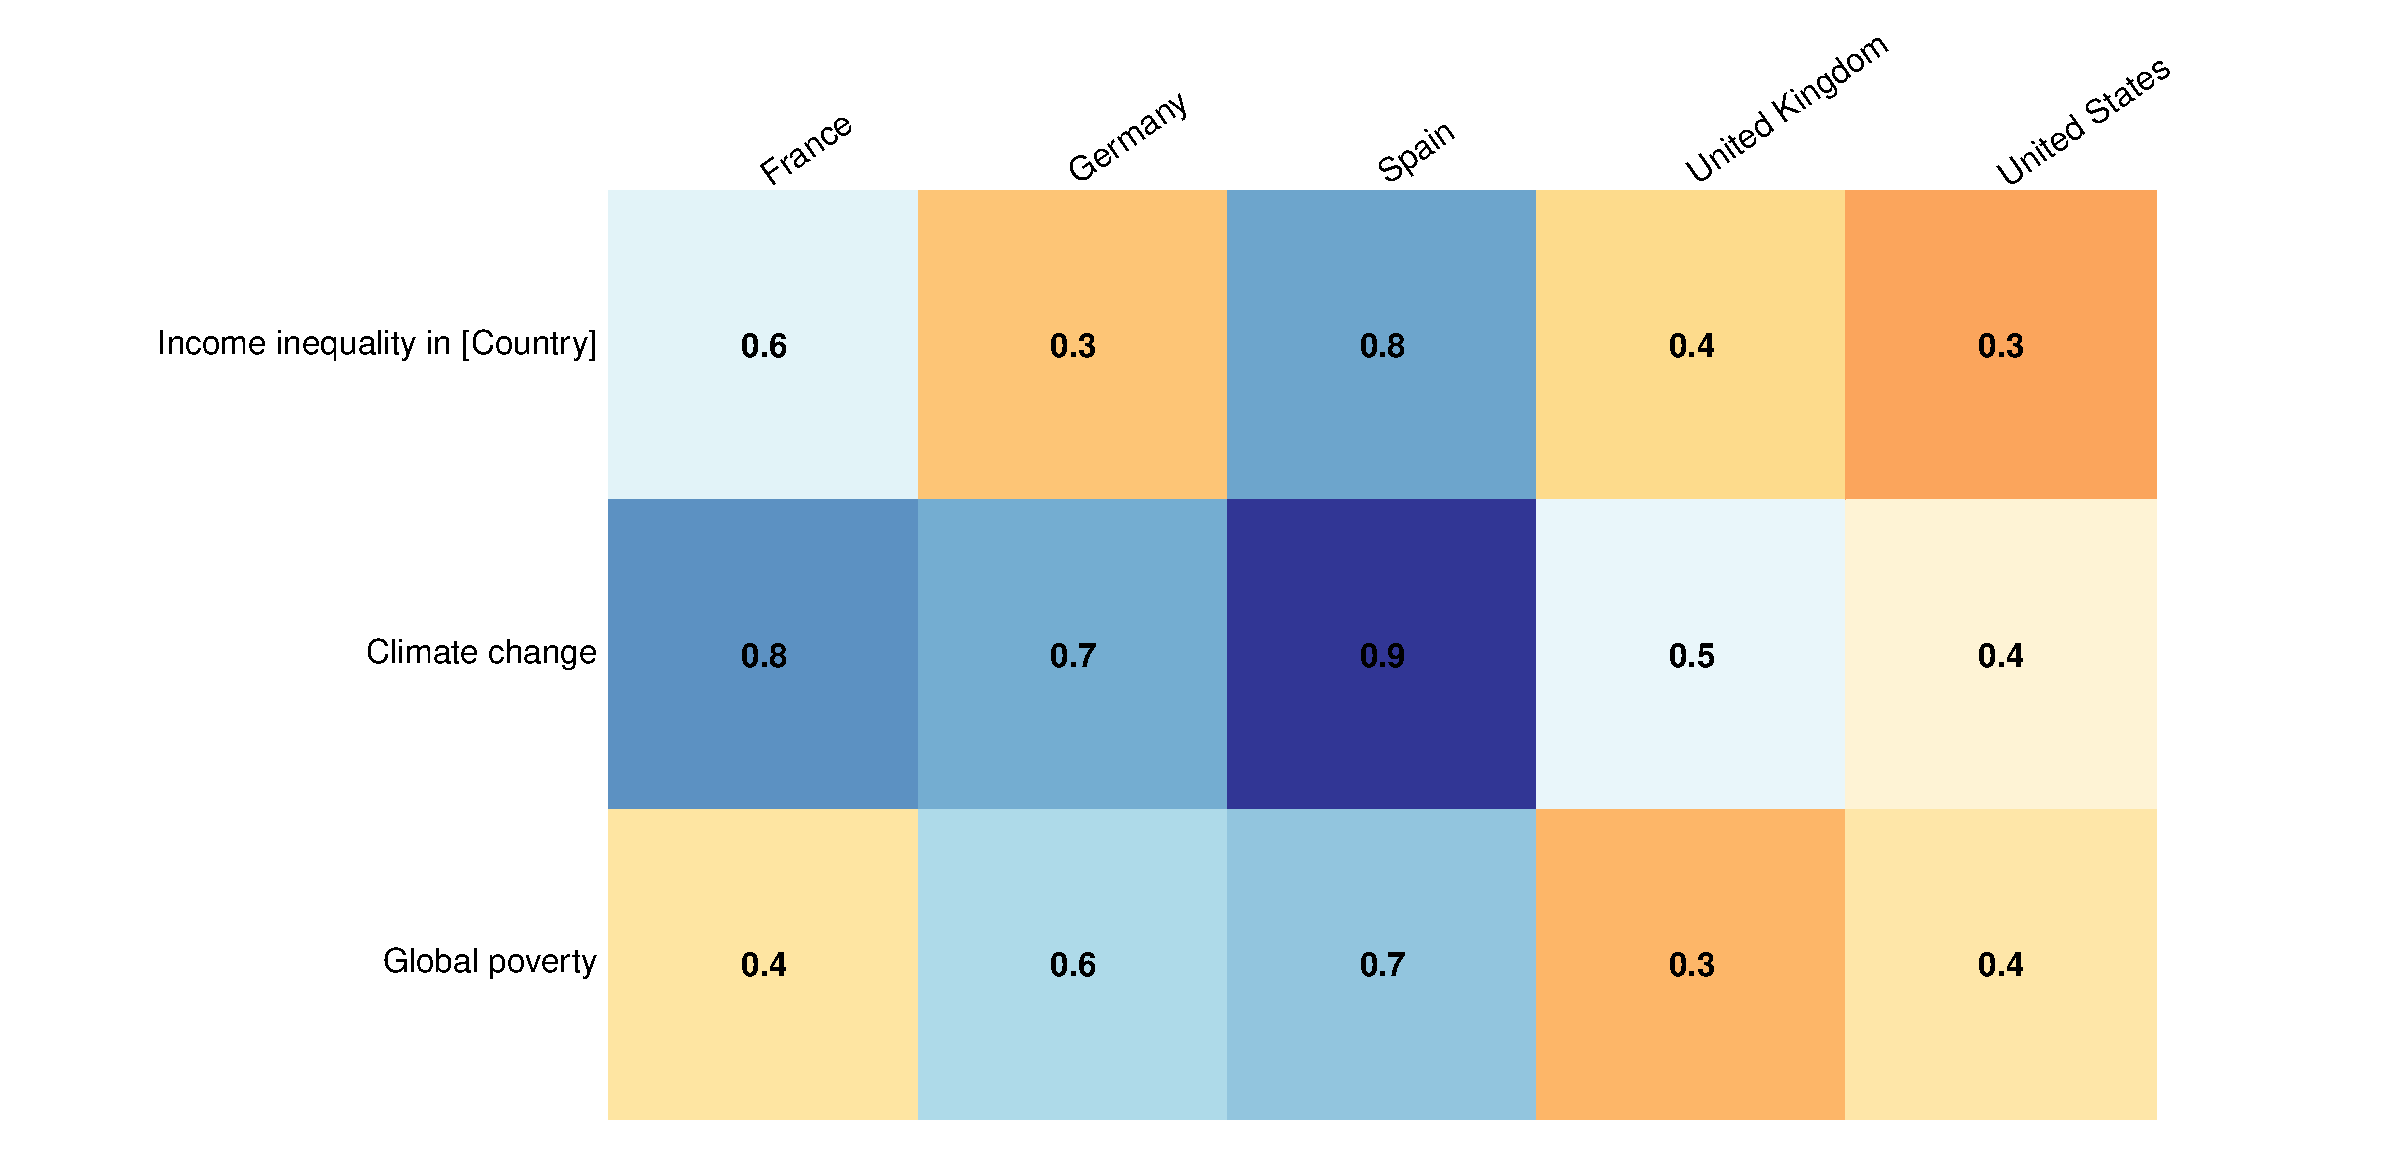
\includegraphics[width=.7\textwidth]{../figures/country_comparison/problem_mean.pdf} 
%     \end{figure}
% 	\bbvs \ip People rank these the importance of these 3 issures as follows: \\ 1. Climate change \\ 2. Global poverty \\ 3. Income inequality in their country
%     \ee
% \end{frame}

\subsection{Wrapping up} 

\begin{frame}{} % Key take-home messages
\begin{itemize}
\ip 1. \rose{Across the world, people are ready for international solidarity} 
	\begin{itemize}
		\item Consensus on the allocation key of emissions permits: equal per capita
        % \item Near consensus for a global tax on millionaires or a global financial register
		% \item Majorities support to channel 30-50\% of global tax revenues to low-income countries
		\item Majorities support global climate policies, including with transfers detrimental to their countries
		% \item Majorities support increased foreign aid if it really helps the poorest
    \end{itemize}
\pause
\ip 2. \rose{The support for global redistributive policies is mostly sincere} 
	\begin{itemize}
		\item Majorities are willing to sign a real-stake petition for the GCS
		% \item The global tax on millionaires is given high priority, the GCS average priority
		\item Progressive candidates would not lose vote by endorsing the GCS
		\item People prefer platforms that include the GCS
	\end{itemize}
\pause
\ip 3. \rose{The mismatch between support and absence of global policies in the public debate remains unexplained} \textit{}
	\begin{itemize}
		% \item Climate change and global poverty are seen as biggest issues than national inequality
		\item Most people show some adherence to universalism
		\item No evidence of pluralistic ignorance: most people correctly guess others' support for the GCS
	\end{itemize} \pause
\ip \blue{Alternative explanations for the mismatch are needed}
    \begin{itemize}
        \item National bias in power structures (elections, media) and mental structures (hymns, sport teams)? %national framing by elections, media, or even sport? 
        %$\Rightarrow$ How to test that?
        \item Pluralistic ignorance of the elites? $\Rightarrow$ Ongoing survey on European Members of Parliament 
        \item Ideas whose time has come, and just lack some advocacy? \pause $\Rightarrow$ I launched a new association: \\ \vspace{.2cm}  \centering 
\includegraphics[height=.08\textheight]{../figures/policies/logo_full}
        %Stay tune for the petition! % Ideas largely accepted but rarely supported?
        % Also: vested interest influence on elites (a la Gillens and Page for the US), cf. Boone story
        % decline of support the more specific a measure gets / enters the public debate
        % people/politicians not believing that other countries (e.g. the U.S.) would accept 
        % people not believing that the policy is technically implementable
        % politicians seeing defects or lack of specification of the policy that warrant opposition, while ignorant citizens would naively like it
        % GCS not lefty enough as it neglects historical responsibility or progressive carbon taxation. It also excludes capacity to pay: imagine decarbonized Norway, they would be net beneficiary from the GCS. => must be completed by other form of redistribution.
        % CAN, after extensive debates among its members, defends the Greenhouse Devlpt Rights (or "Fair Share") approach, so they will attack the GCS. => Important to frame our results in broad terms (people support global redistribution) rather than specific terms (support GCS). Then say it's important that high-income countries' diplomats change their approach of negotiations and study any proposal, be it GDR, GCS, or something else. Same for the petition, perhaps not in favor of GCS, but in favor of binding climate agreement with flows from high- to low-income countries of at least 1% of GDP.
    \end{itemize}
\end{itemize}
\end{frame}

\section{The Global Climate Plan}

\begin{frame}{An old idea}
    \bbvsp \ip \blue{Grubb (1990), Agarwal \& Narain (1991) and Bertram (1992)} were the first advocates of an equal right to emit for each human. 
    \ip \blue{Grubb (1990)}: ``\textit{by far the best combination of long term effectiveness, feasibility, equity, and simplicity, is obtained from a system based upon tradable permits for carbon emission which are allocated on an adult per capita basis}''.
    \ip A support renewed ever since: \blue{Baer et al. (2000), Jamieson (2001), Rajan (2021)}. 
    \ip In \blue{Cramton et al. (2015)}, all agree for a climate club with international transfers.
    \ip \blue{Gollier \& Tirole (2015)} synthesize the distributional decision with a \textit{generosity} parameter, from grandfathering to equal per capita. % \citet{gollier_negotiating_2015} synthesize the distributional decision with a \textit{generosity} parameter which would allocate emissions permit to countries in proportion to their population if set to one, in proportion to their emissions (on the start date of the policy) if set to zero, and as a mixture of the egalitarian and grandfathering rules if set in between.
    \ip \blue{Cramton et al. (2015)} propose that \textit{average} countries fix the generosity, and to set the tax rate at the minimum price proposed by participating countries. % Using a similar formula in the context of a tax, \citet{cramton_international_2015} (summarized in \citealp{mackay_price_2015}) propose that countries around the average emission per capita fix the generosity parameter, so that it is strategically chosen to maximize the tax rate, and to fix the tax rate at the minimum price proposed by participating countries. Negotiations would exclude countries with low ambition beforehand; and the treaty would impose trade sanctions on non-participating countries.
    \ip \blue{van den Bergh et al. (2020)} propose an expanding climate club and a reorientation of COP negotiations. % \citet{bergh_dual-track_2020} propose a ``dual-track transition to global carbon pricing'': an expanding climate club that would integrate existing and new emissions trading systems, and a reorientation of UNFCCC negotiations towards a global carbon price and burden-sharing rules. 
    \ip The \blue{IMF (2019)} propose either differentiated prices among countries or international transfers. % with a carbon price floor as a first step
    \ip \blue{Carattini et al. (2019)} find support of $\approx$80\% in India and $\approx$50\% in the U.S., UK, Australia for a global tax and dividend.
    \ee
\end{frame}

\begin{frame}{The trajectories}
    \begin{figure}
        \centering 
        \caption{Global trajectories estimated for the Global Climate Plan (GCP)
        }
        \only<1>{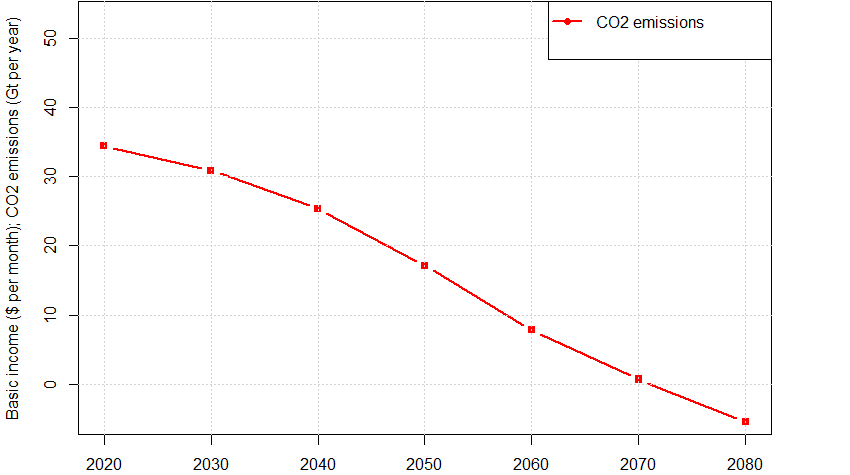
\includegraphics[height=.8\textheight]{../figures/policies/trajectory_emissions} }
        \only<2>{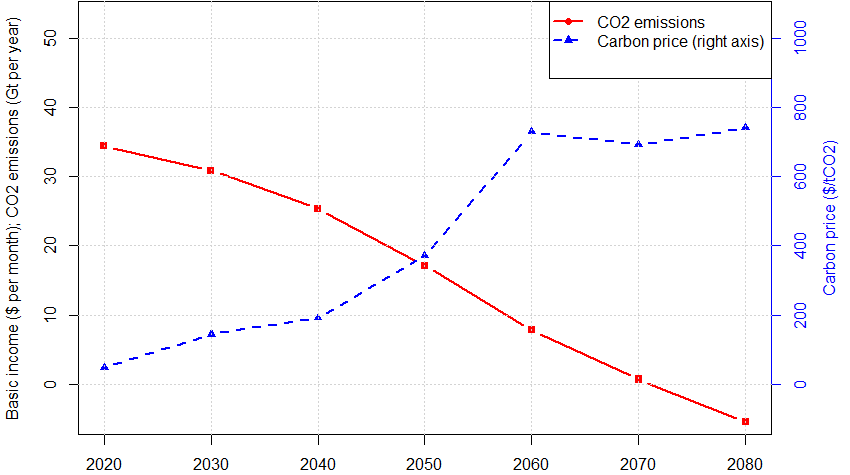
\includegraphics[height=.8\textheight]{../figures/policies/trajectory_price}  }
        \only<3>{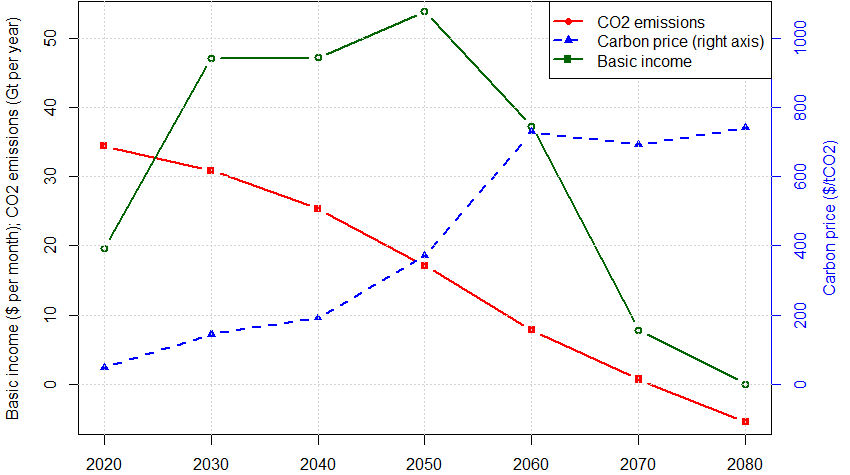
\includegraphics[height=.8\textheight]{../figures/policies/trajectory_full}  }
    \end{figure}    
\end{frame}

\begin{frame}{The principles}
    \begin{enumerate}[<+->]
        \item \blue{A cap on emissions to meet the 2\textdegree{}C target.}
        \bbvsp \ip $\Rightarrow$ Define a carbon budget and an emissions trajectory.
        \ip ETSs already cover 17\% of global GHG emissions (EU, China, South Korea...), are considered in various countries (India, Brazil, Nigeria).
        \ee
        \item \blue{A global basic income that eradicates extreme poverty.}
        \bbvsp \ip At their peak, GCP revenues at 5\% of world GDP, with 1\% of world GDP in international transfers. 
        \ip The basic income of $\approx$\$50 per month (in nominal) for each human above 15 would lift out of extreme poverty the 700 million people with less than \$2.15 a day (in PPP).
        \ee
        \item \blue{A climate club to foster global cooperation.}
        \bbvsp \ip Entry into force when signatories cover 60\% of global emissions.
        \ip A carbon border adjustment. \ee % TODO! detail BCA
    \end{enumerate}
\end{frame}

\begin{frame}{The unadjusted distributive effects}
    \begin{figure}
        \centering 
        \caption{Distributive effects of the Global Climate Scheme in 2030.}
        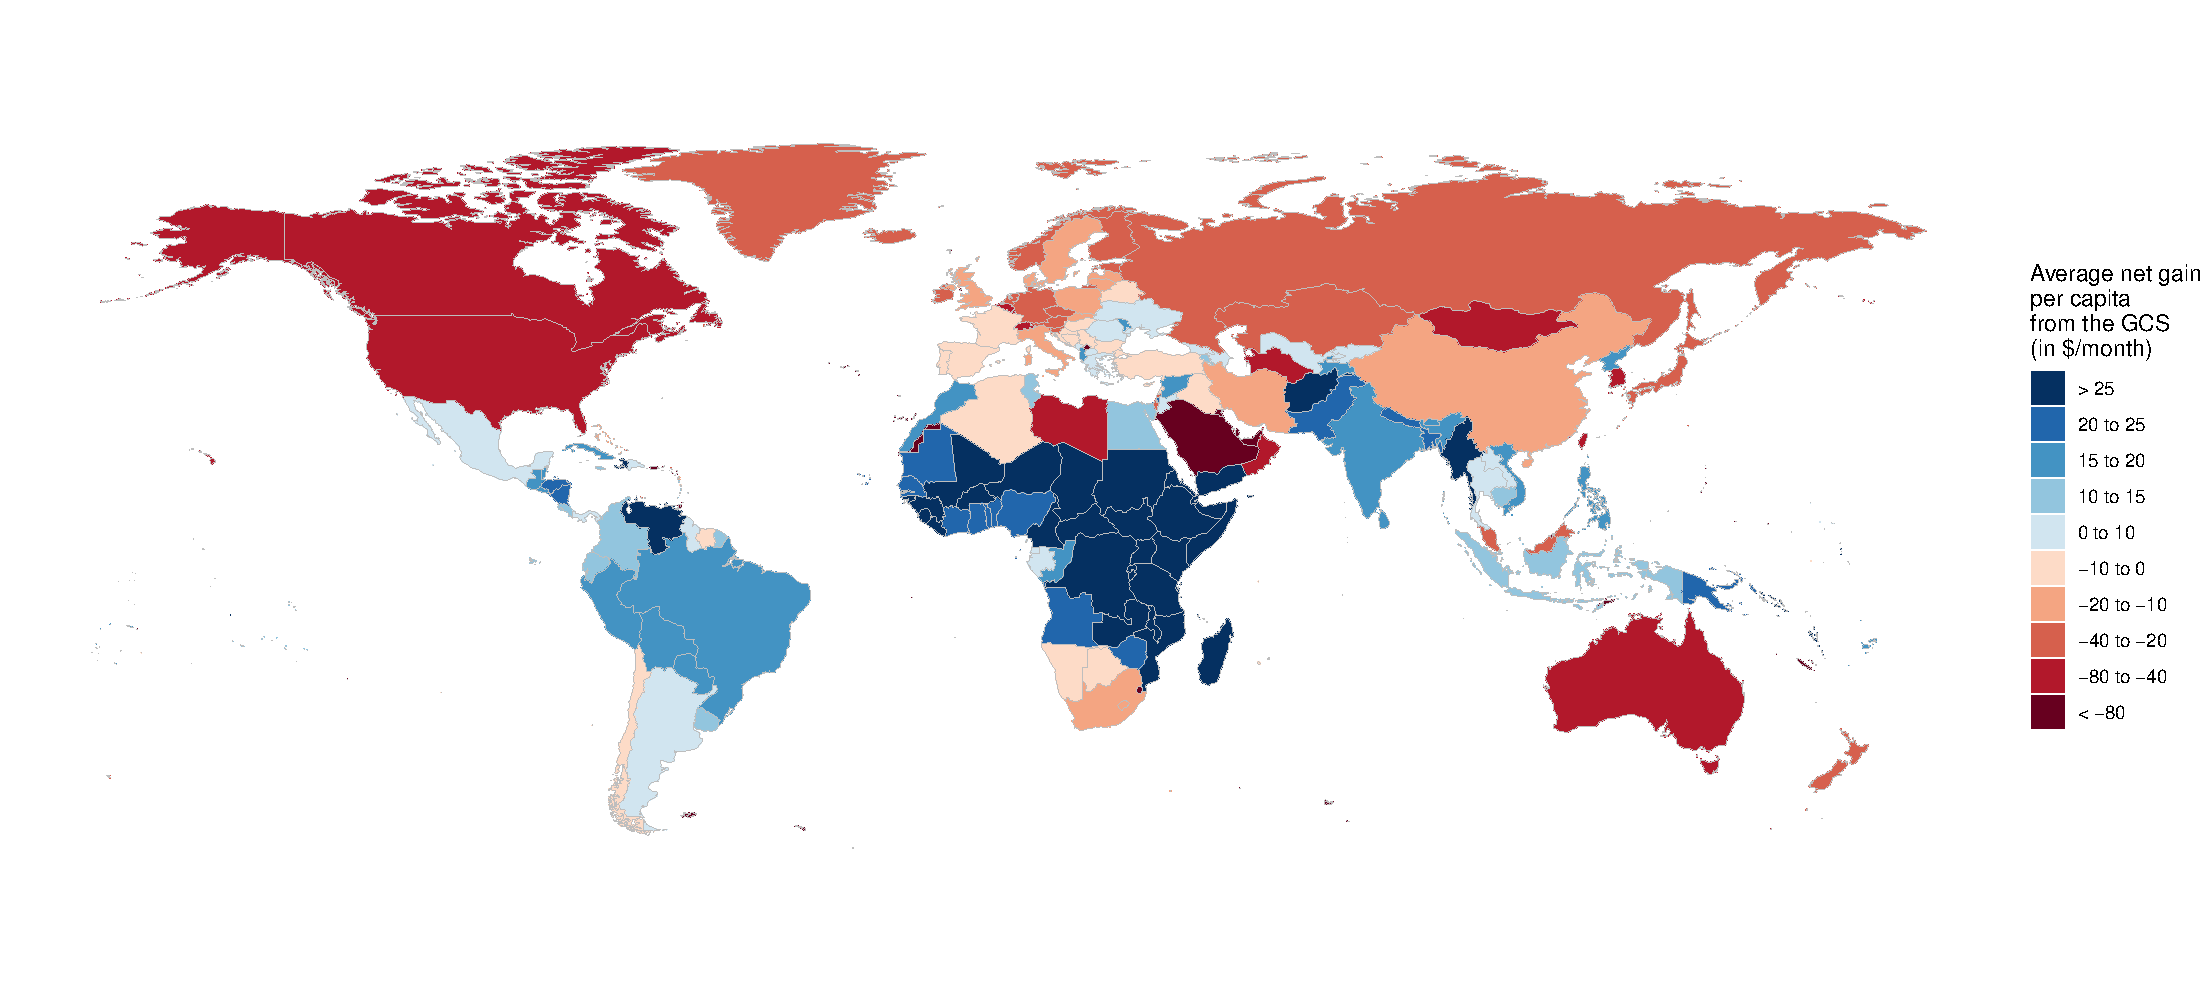
\includegraphics[height=.8\textheight]{../figures/maps/mean_gain_2030.pdf} 
    \end{figure}        
\end{frame}

\begin{frame}{Participation mechanisms}
    \bbsp 
    \ip An \textit{opt out} provision to account for the ability to pay.
    \bbvsp \ip Middle-income countries with higher-than-average carbon footprint can opt out from the mutualization of revenues.
        \ip Opting out countries retain the auction revenues they collect.
        \ip Full opt out authorized up to 1.5 times world average GDP p.c. 
        \ip Opt out right is phased out between 1.5 and 2 times world average GDP p.c. 
        \ip \blue{$\Rightarrow$ China, Iran, South Africa... would not lose from the Global Climate \textit{Plan}.}
        \ee
    \ip Provisions to accommodate subnational entities into the club.
    \bbvsp \ip They can opt out from the carbon border adjustment.
        \ip They can use their revenues as they please.
        \ip $\Rightarrow$ The states of California, New York, Illinois, Massachusetts... could join.% 40\% of U.S. GDP
        \ee
    \ip A provision to avoid anti-redistributive effects.
    \bbvsp \ip High-income countries with a lower-than-average carbon footprint would not receive any revenues.
        \ee
    \ee
\end{frame}

\begin{frame}{The distributive effects\label{distributive}}
    \begin{figure}
        \centering 
        \only<1>{ \caption{Distributive effects of the Global Climate Plan in 2030.   \hyperlink{other_distributive}{\beamergotobutton{More maps}}}
        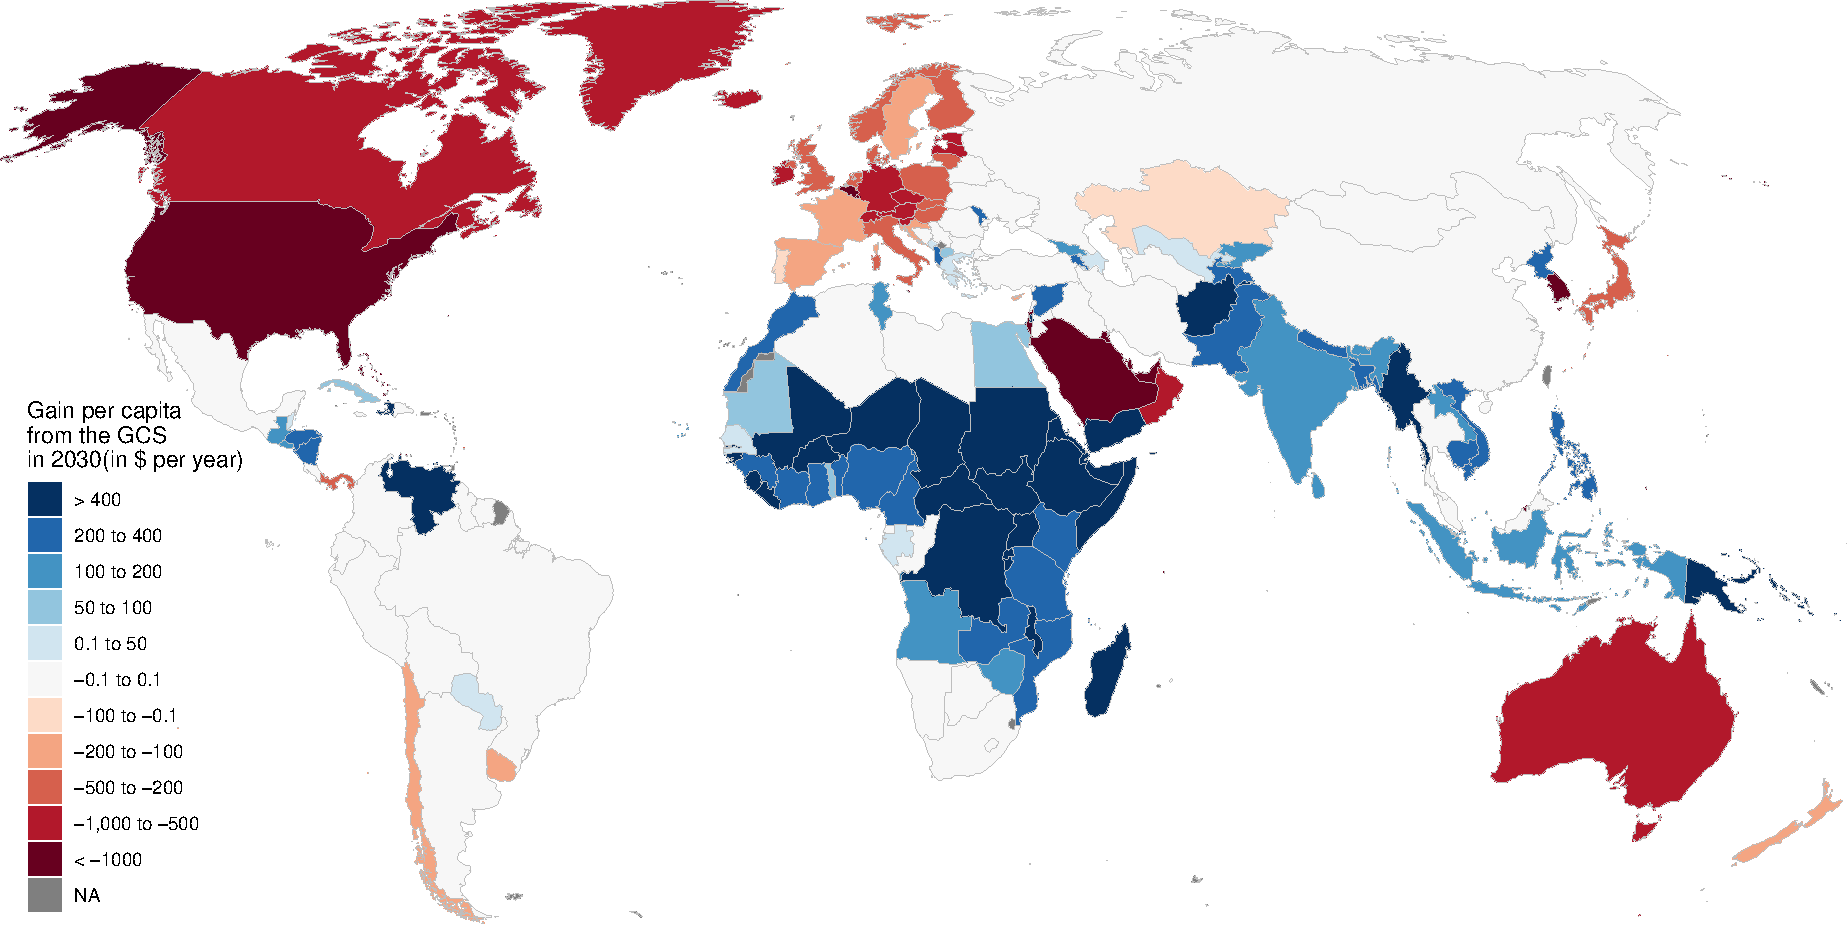
\includegraphics[height=.8\textheight]{../figures/maps/gain_adj_2030.pdf}}
        % \only<2>{ \caption{Distributive effects of the Global Climate Plan in 2030.}
        % 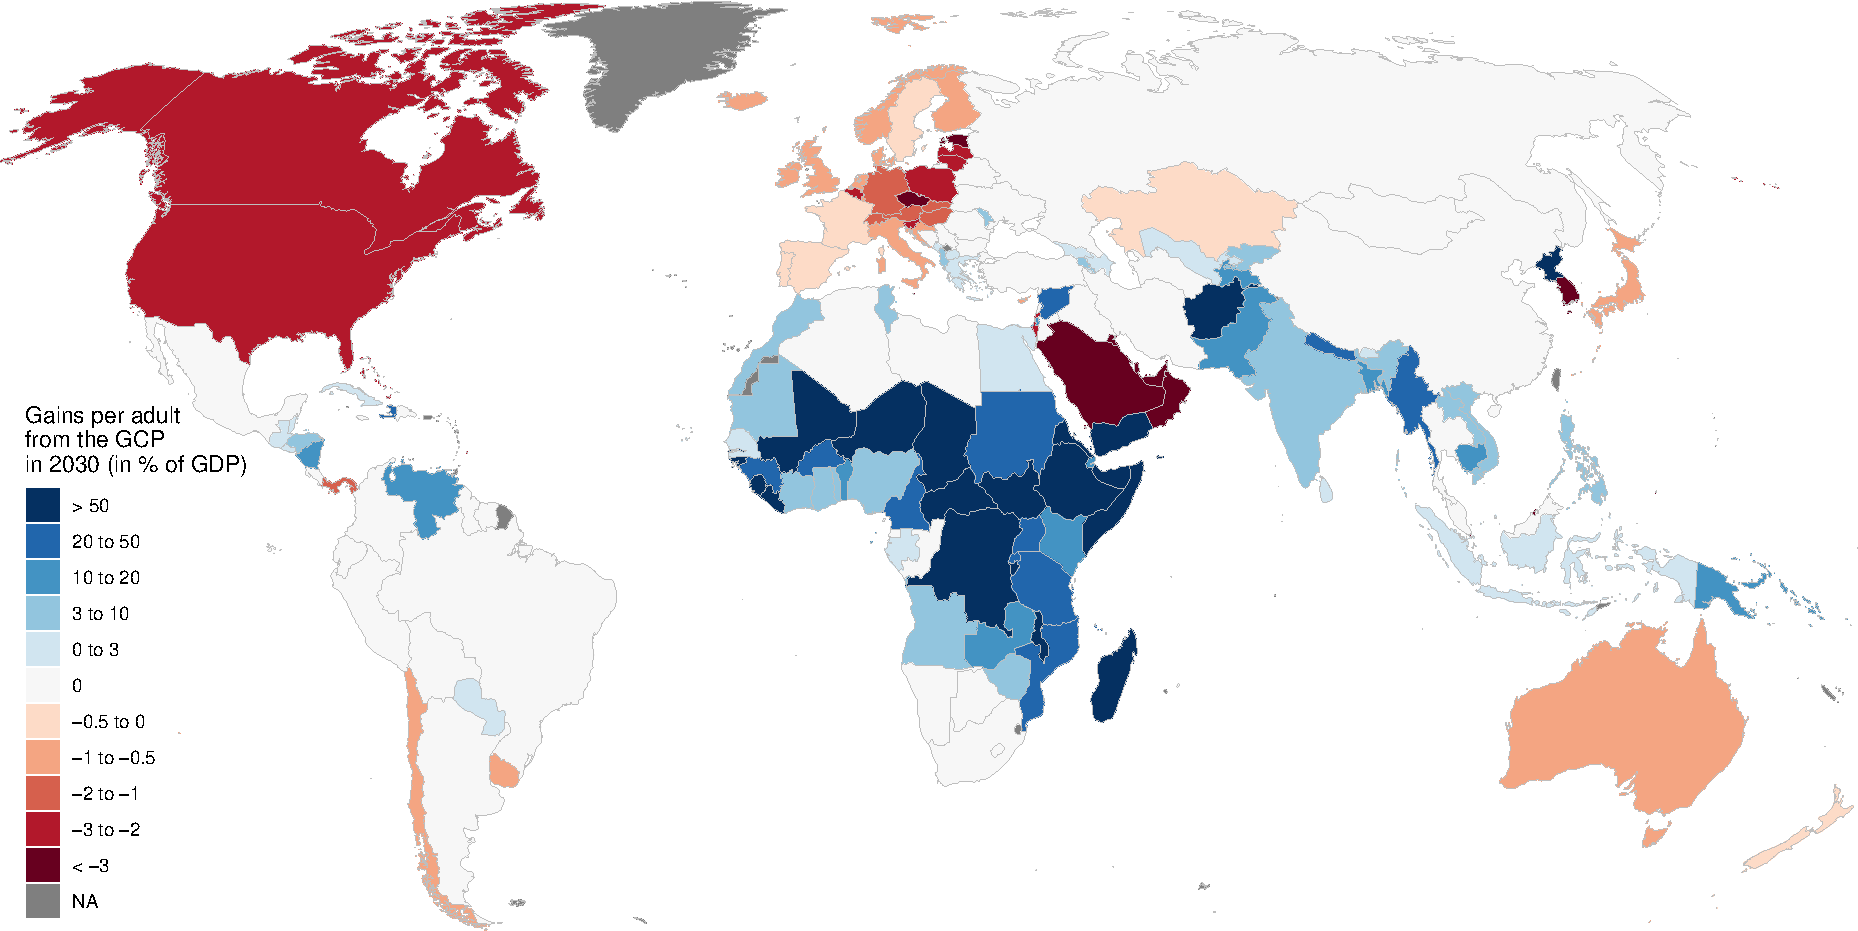
\includegraphics[height=.8\textheight]{../figures/maps/gain_adj_over_gdp_2030.pdf} } % TODO! more slides
        \only<2>{ \caption{Distributive effects of the Global Climate Plan throughout the century. \hyperlink{other_distributive}{\beamergotobutton{More maps}}}
        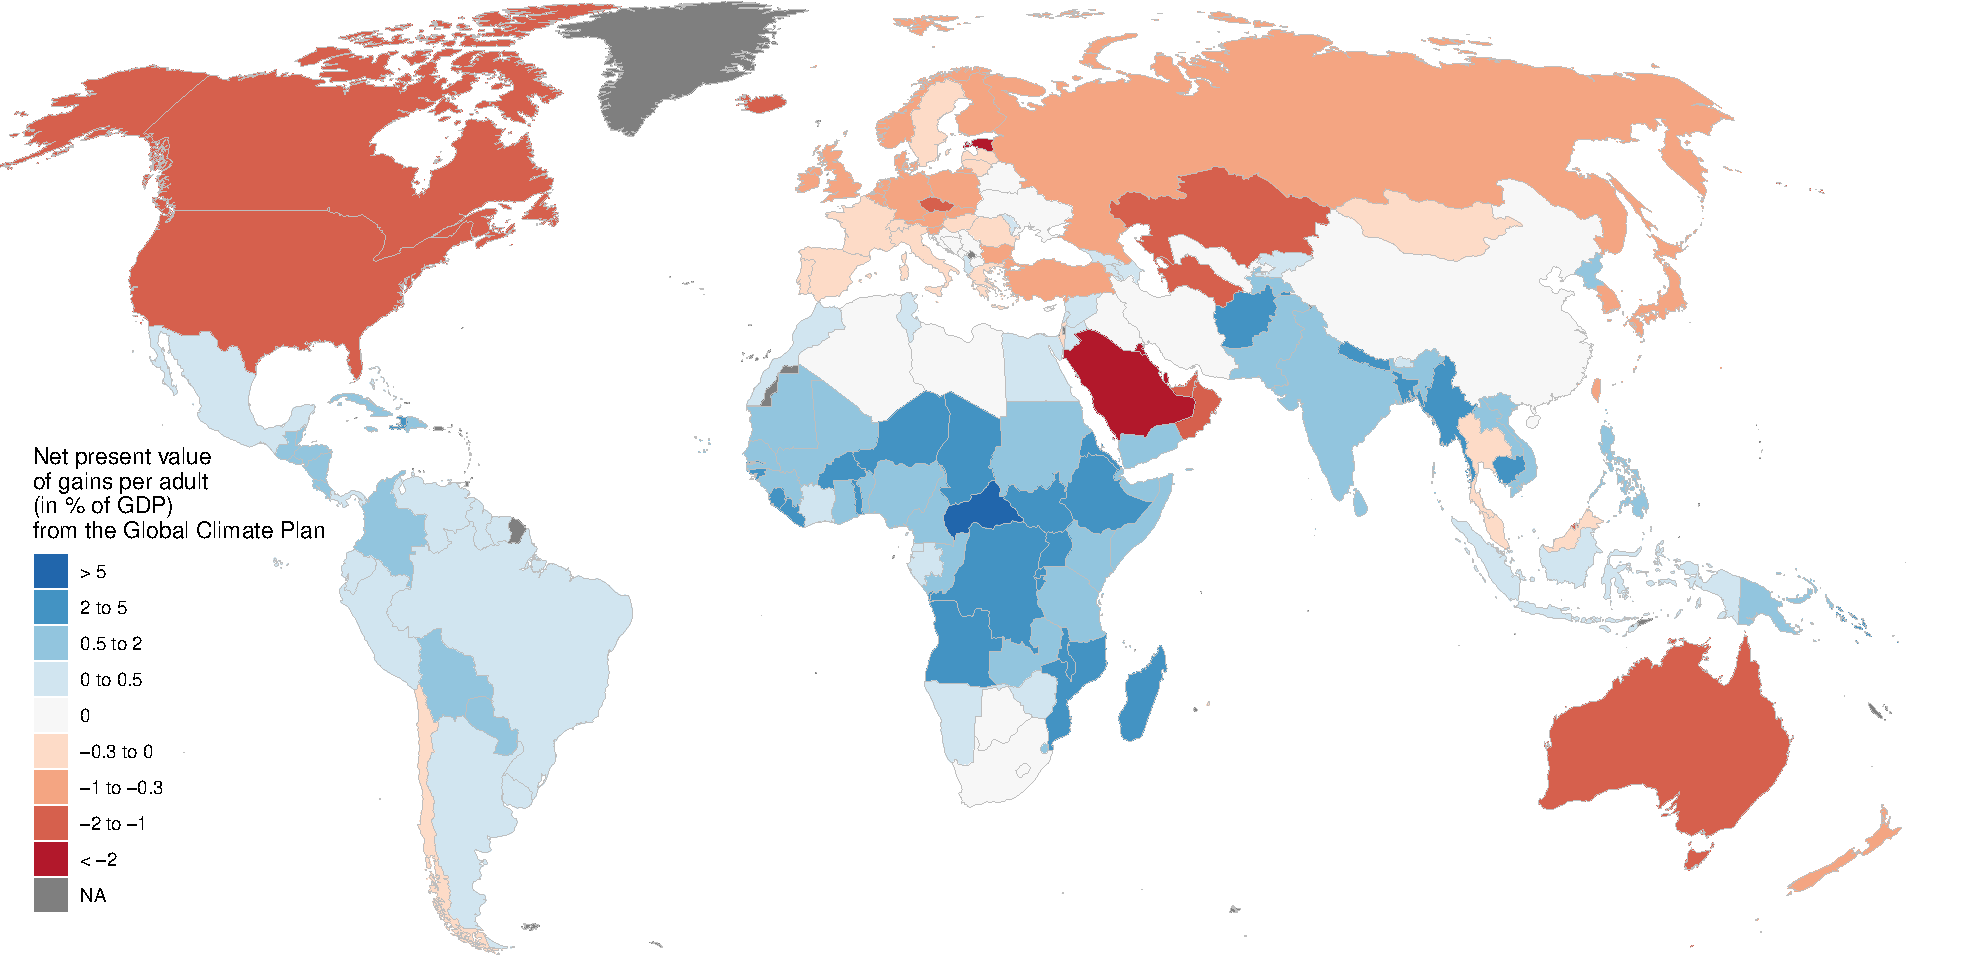
\includegraphics[height=.8\textheight]{../figures/maps/npv_over_gdp_gcs_adj.pdf} }
    \end{figure}        
\end{frame}

\begin{frame}{Complementarity with others policies}
    \bbsp \ip The basic income increases the fiscal capacity of \blue{low-income countries}, which \blue{can raise taxes} to fund public services and infrastructures.
    \ip Other sources of funding (e.g. a global corporate tax) should \blue{sustain the basic income in the long run}.
    \ip \rose{A global wealth tax financing (at least in part) low-income countries can address historical responsibilities}.
    \ip In high-income countries, \rose{national redistribution} can offset the negative incidence on median emitters.
    \ip The GCP fosters \rose{national climate policies} (investments, subsidies, norms):
        \bbsp \ip Lowering a country's emissions reduces what it pays to the rest of the world.
        \ip By mutualizing some decarbonization costs, national climate policies can reduce horizontal inequalities (discrepancies in private costs between individuals with similar income but different carbon footprints).
        \ee
    \ip A \blue{global democratic climate assembly} would be the ideal forum for climate governance.
    \ee
\end{frame}

\begin{frame}{Implementation}
    \bbsp \ip Need to monitor, report and verify emissions of industrial units.
        \bbsp \ip Challenging to avoid fraud in countries lacking institutional capacity, but same for any climate policy.
        \ip The GCP would provide resources and assistance from experienced countries. \ee
    \ip Distributing a global basic income is challenging: need to reach everyone and avoid fraud.
        \bbsp \ip Most countries maintain electoral lists and already have social programs for isolated people.
        \ip Smartphones can provide biometric identification and means of transaction.
        \ip Satellite internet access might soon become cheap and ubiquitous (Hanson 2016).
        \ee
    \ee 
\end{frame}

\begin{frame}{Details}
    \bbsp \ip \textbf{Ideal timeline}: negotiation, consultations up to 2030, phase-in between 2030 and 2035.
    \ip \textbf{Scope}: ideally, all CO$_\text{2}$. Initially, CO$_\text{2}$ from fossil fuels and cement production in large industrial units, including shipping and aviation.
    \ip \textbf{Framework}: defines the scope, use of revenues, rules of governance, and \blue{carbon budget} (e.g. 500 GtCO$_\text{2}$ from 2030 $\approx$ $<+2$\textdegree{}C with 67\% chance).
    \ip \textbf{Governance}: the governing body would choose the yearly emissions quota, the market design, and possible sanctions against non-participating or non-complying entities. % Voting rights proportional to emissions
    \ip \textbf{Market design}: Carbon offsets should not be allowed. Borrowing and banking emissions permits should be limited.
    \ee
\end{frame}

\begin{frame}{We need you!}
    \begin{figure}
        \centering \caption{You liked the GCP? \href{https://github.com/bixiou/global_tax_attitudes/raw/main/paper/policy_brief_GCS.pdf}{Read}, share, endorse on \rose{\href{https://global-redistribution-advocates.org/the-global-climate-plan/}{global-redistribution-advocates.org}}!}
        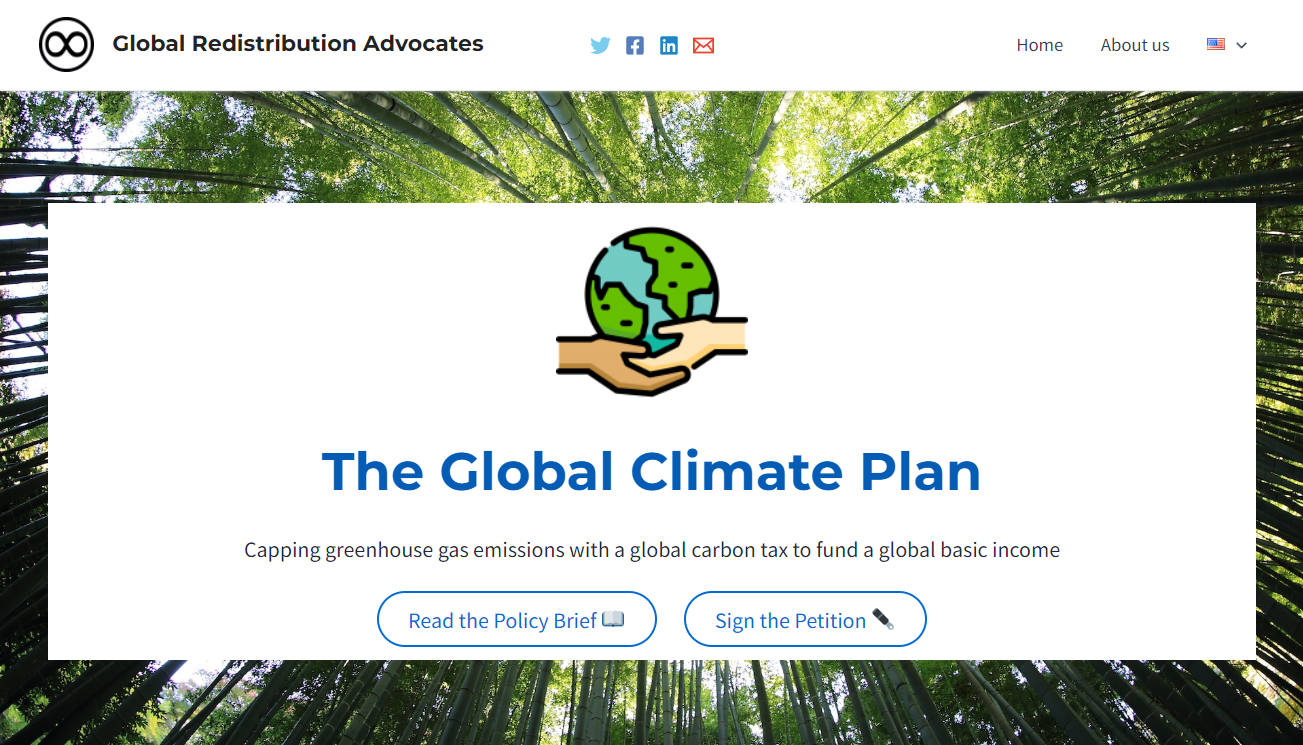
\includegraphics[height=.55\textheight]{../figures/policies/petition.PNG} 
    \end{figure}    
    \bbsp \ip \quad \quad \quad \quad \quad \quad Want to help? \pause We need specialists for the GCP's scientific committee.
    \ip \pause \quad \quad \quad \quad \quad \quad Have comments or criticisms? \pause Happy to take any question or remark!
    \ip \hspace{6.5cm} \href{https://youtu.be/Bypt4H8K5dI?t=106s}{\beamergotobutton{Video}}
    \ee
\end{frame}

\appendix
\section{Appendix}

\subsection{Additional results}

% TODO appendix
% \begin{frame}{Support for increased foreign aid\label{}}\vspace{-.2cm} 
%     \begin{figure} 
%         \centering 
%         \caption{Actual, perceived and preferred amount of foreign aid, with random info (or not) on actual amount. (\textit{Mean})}\vspace{-.2cm}
%         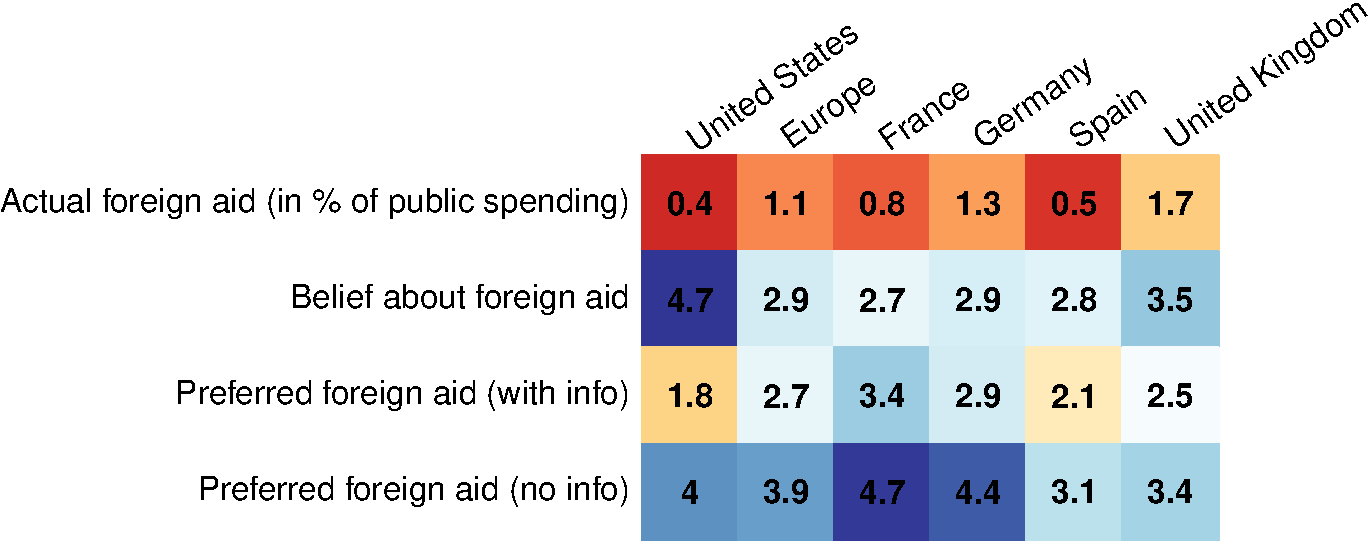
\includegraphics[height=.4\textheight]{../figures/country_comparison/foreign_aid_amount_mean.pdf} % TODO: see median
%     \end{figure}\vspace{-.2cm}\pause
%     \begin{figure} 
%         \centering 
%         % \caption{Support for increased foreign aid (vs. reduced or stable): from previous question, and directly asked (with info).}\vspace{-.2cm}
%         % 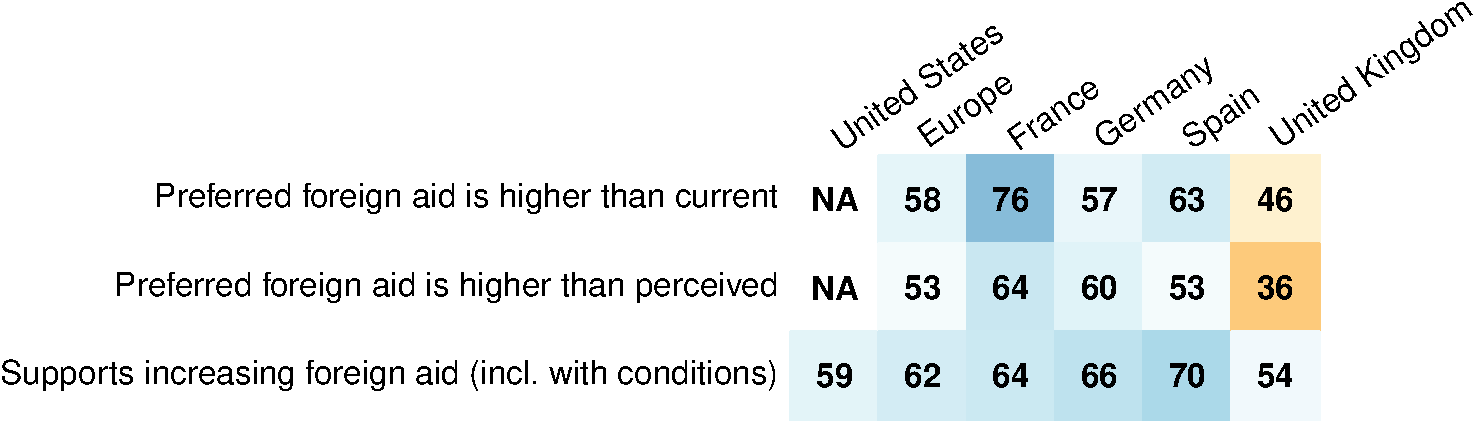
\includegraphics[height=.32\textheight]{../figures/country_comparison/foreign_aid_more_positive.pdf} 
%         \caption{Support for increased foreign aid: from previous question, and directly asked (with info).}\vspace{-.2cm}
%         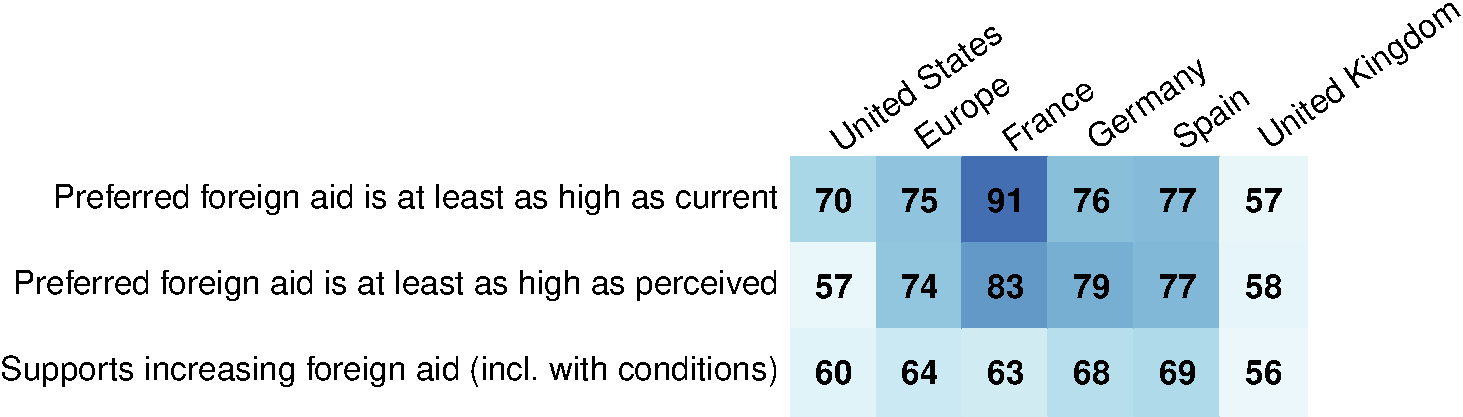
\includegraphics[height=.32\textheight]{../figures/country_comparison/foreign_aid_no_less_positive.pdf} 
%     \end{figure} \vspace{-.1cm}
% 	\quad \quad \quad \quad \quad \quad \blue{Actual foreign aid is overestimated.} \quad \quad \quad \rose{Majorities support more foreign aid.}
% \end{frame}

\begin{frame}{Conditions for increased foreign aid \label{foreign_aid_conditions} \hyperlink{other_policies}{\beamergotobutton{Go back}}}
    \begin{figure} \vspace{-.2cm}
        \centering 
        \caption{[Info on actual amount]. Do you support [the U.S.] transferring more money to low-income countries?}\vspace{-.2cm}
        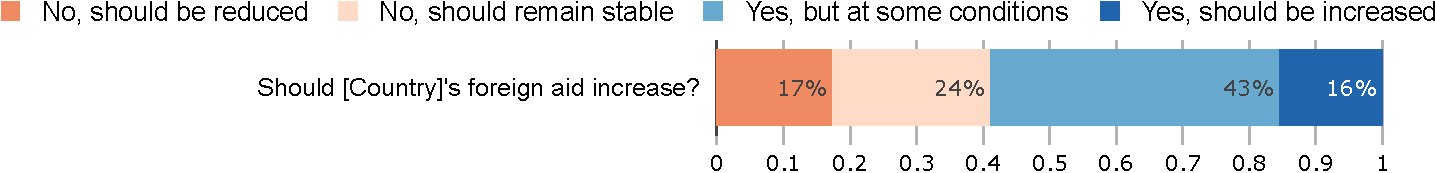
\includegraphics[width=.7\textwidth]{../figures/all/foreign_aid_raise_support.pdf} 
    \end{figure}\vspace{-.2cm} \pause
    \begin{figure} 
        \centering 
        \caption{[If \textit{at some conditions}] What conditions should be required for [the U.S.] to increase its foreign aid?}\vspace{-.2cm}
        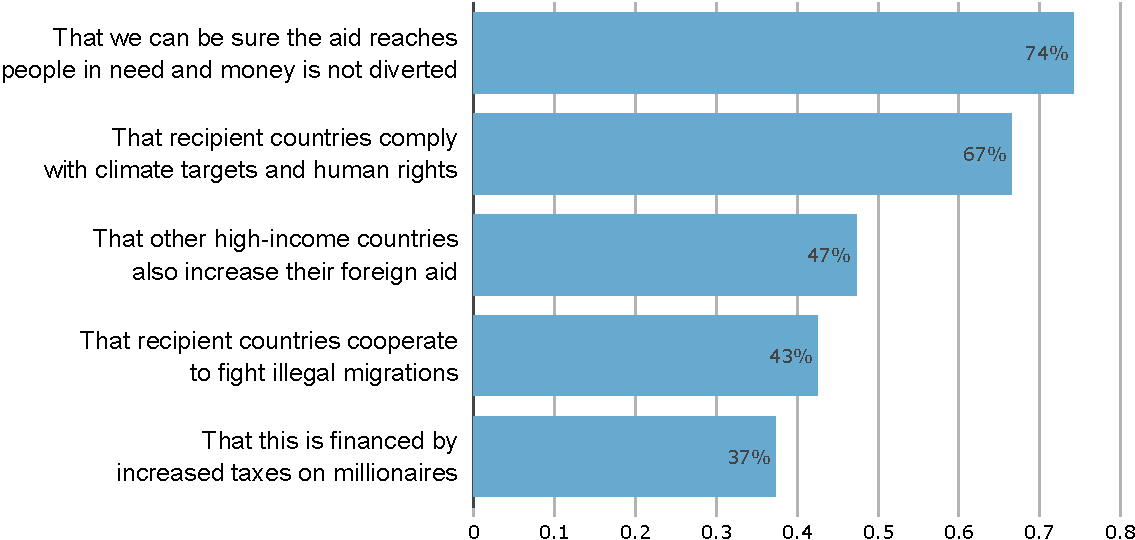
\includegraphics[height=.48\textheight]{../figures/all/foreign_aid_condition.pdf} 
    \end{figure} \pause \vspace{-.3cm}
	\bbvs \ip \blue{People want to help people (not oligarchs) and to foster climate action and human rights.}% sustainability.
	\ip National preference is the main reason behind not wanting increased foreign aid.
	\ee 
\end{frame}

\begin{frame}{Preferences over public spending%How to fund increased foreign aid
	\hyperlink{other_policies}{\beamergotobutton{Go back}}}
	\begin{columns}
        \begin{column}{0.5\textwidth}
            \begin{figure}
				\vspace{-.2cm}
                \centering 
                \caption{Your previous answer shows that you would like to increase [UK] foreign aid.\\How would you like to finance such increase in foreign aid? (Multiple answers possible)}
                \vspace{-.2cm}
                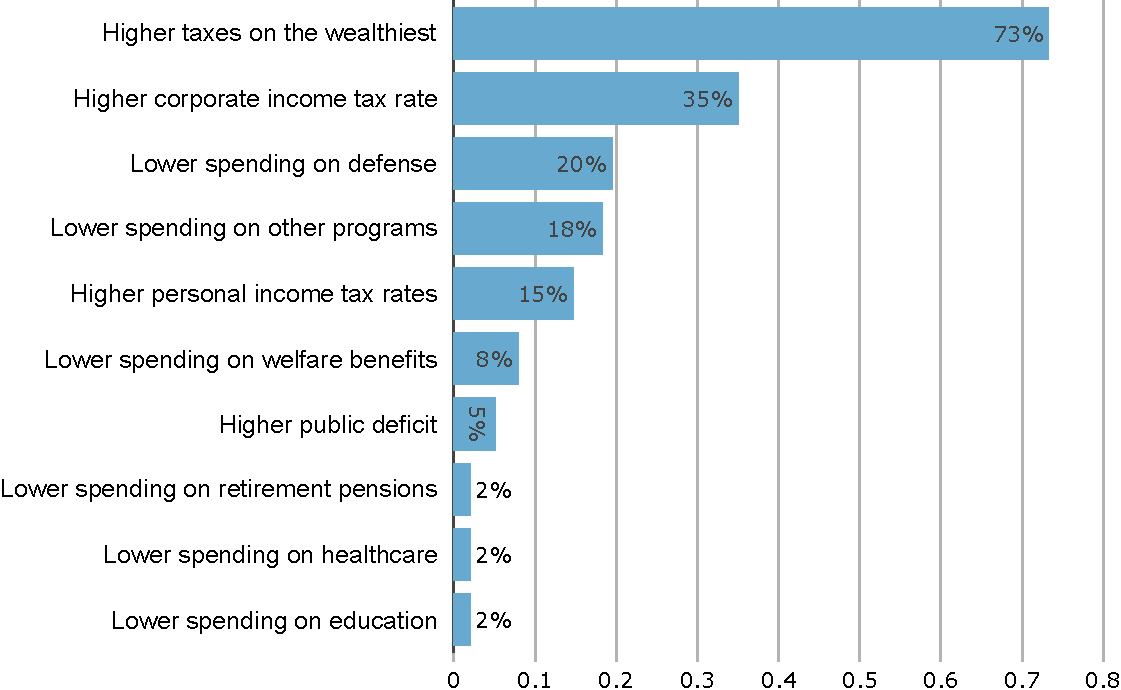
\includegraphics[width=\columnwidth]{../figures/all/foreign_aid_raise.pdf} 
            \end{figure}
        \end{column}
        \begin{column}{0.5\textwidth}			
            \begin{figure}\vspace{-.2cm}
                \centering 
                \caption{Your previous answer shows that you would like to reduce [UK] foreign aid.\\How would you like to use the freed budget? (Multiple answers possible)}
                \vspace{-.2cm}
                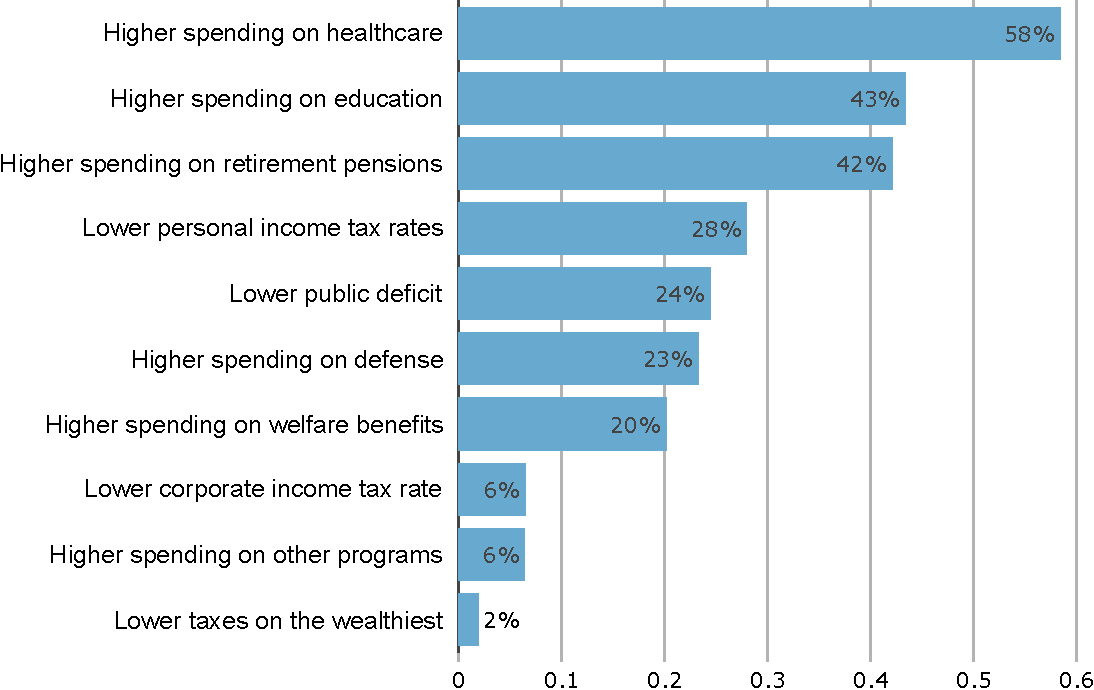
\includegraphics[width=\columnwidth]{../figures/all/foreign_aid_reduce.pdf} 
            \end{figure}
        \end{column}
    \end{columns}
	\bbvs \ip \rose{People want better public services and higher taxes on the wealthiest.}
	\ee 
\end{frame} 

\begin{frame}{Support for increased foreign aid \hyperlink{other_policies}{\beamergotobutton{Go back}}\label{foreign_aid_perceptions}}\vspace{-.2cm} 
    \begin{figure} 
        \centering 
        \caption{Actual, perceived and preferred amount of foreign aid, with random info (or not) on actual amount. (\textit{Mean})}\vspace{-.2cm}
        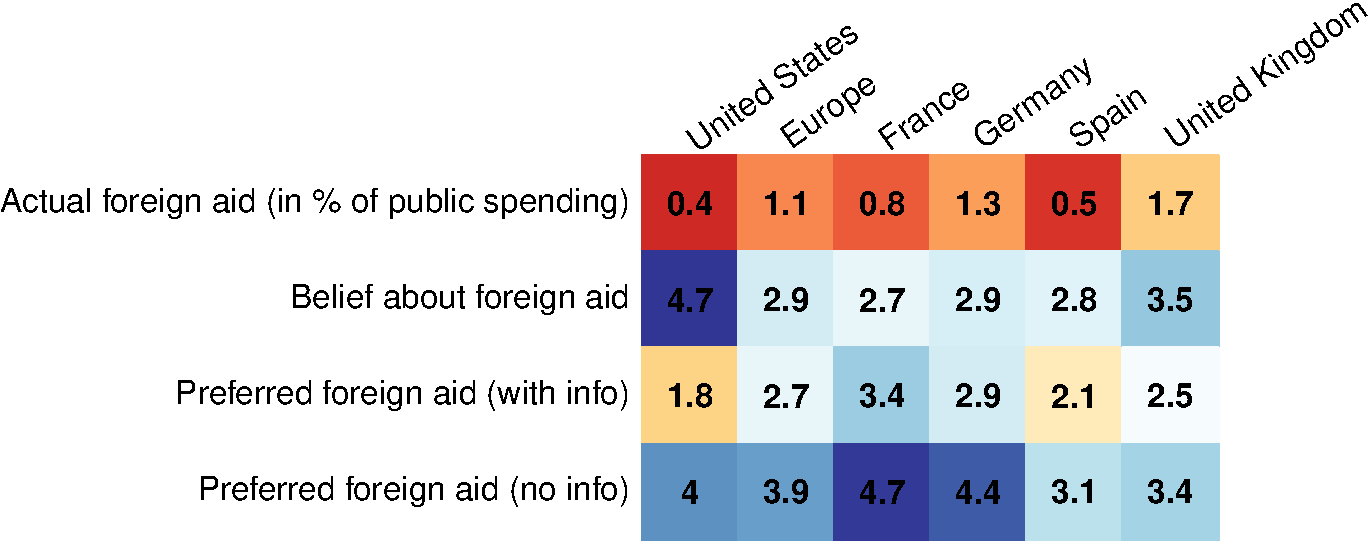
\includegraphics[height=.4\textheight]{../figures/country_comparison/foreign_aid_amount_mean.pdf} % TODO: see median
    \end{figure}\vspace{-.2cm}\pause
    \begin{figure} 
        \centering 
        % \caption{Support for increased foreign aid (vs. reduced or stable): from previous question, and directly asked (with info).}\vspace{-.2cm}
        % 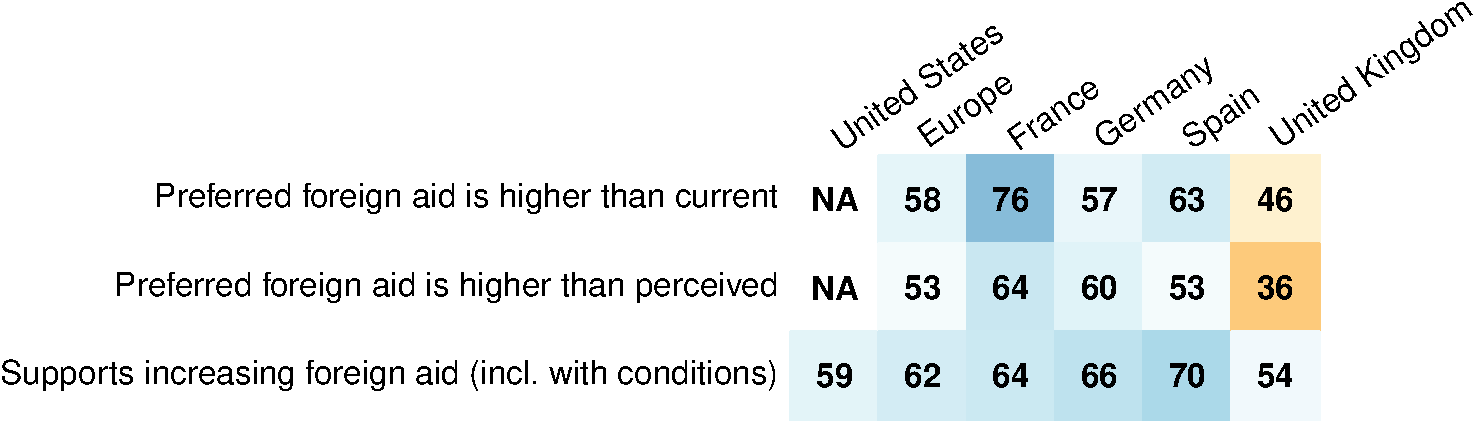
\includegraphics[height=.32\textheight]{../figures/country_comparison/foreign_aid_more_positive.pdf} 
        \caption{Support for increased foreign aid: from previous question, and directly asked (with info).}\vspace{-.2cm}
        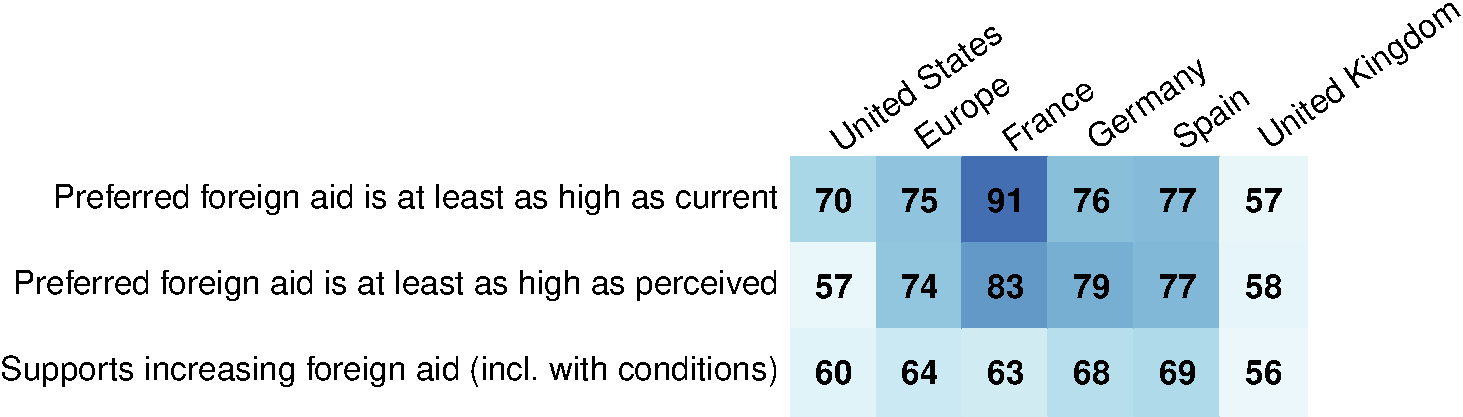
\includegraphics[height=.32\textheight]{../figures/country_comparison/foreign_aid_no_less_positive.pdf} 
    \end{figure} \vspace{-.1cm}
	\quad \quad \quad \quad \quad \quad \blue{Actual foreign aid is overestimated.} \quad \quad \quad \rose{Majorities support more foreign aid.}
\end{frame}

\begin{frame}{Perceptions of the Global Climate Scheme \hyperlink{gcs_support}{\beamergotobutton{Go back}}\label{gcs_perceptions}}
	\vspace{-.3cm}
    \begin{figure}
        \centering 
        \caption{When determining your support or opposition to the Global climate scheme, which points are important to you?}
        \vspace{-.2cm}
        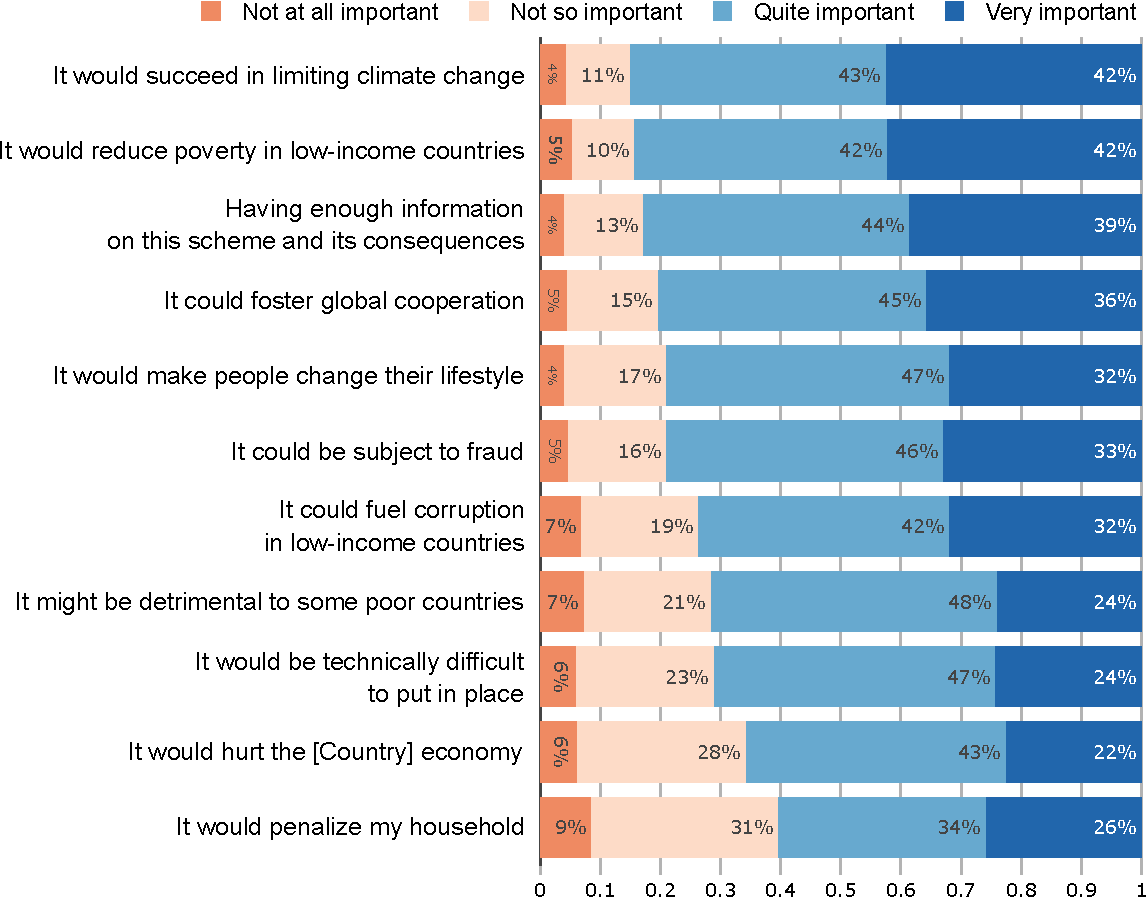
\includegraphics[height=.9\textheight]{../figures/all/gcs_important.pdf} 
    \end{figure}
\end{frame}

\begin{frame}{Conjoint analyses: interaction with other policies \hyperlink{gcs_support}{\beamergotobutton{Go back}}\label{conjoint_ab}} 
    \bbvs \ip National climate policy (C) is as supported as the GCS, but no substitute for it.
	\ip Support for the GCS does not increase when complemented by National Redistribution.
	\ip $\Rightarrow$ Confirms that the \rose{monetary loss is not a primary concern} for one's attitude toward the GCS.
    \ee
    \begin{figure} \vspace*{-.5cm}
        \centering 
        \caption{Among the two following bundles of policies, which one would you prefer?}
        \vspace{-.2cm} 
        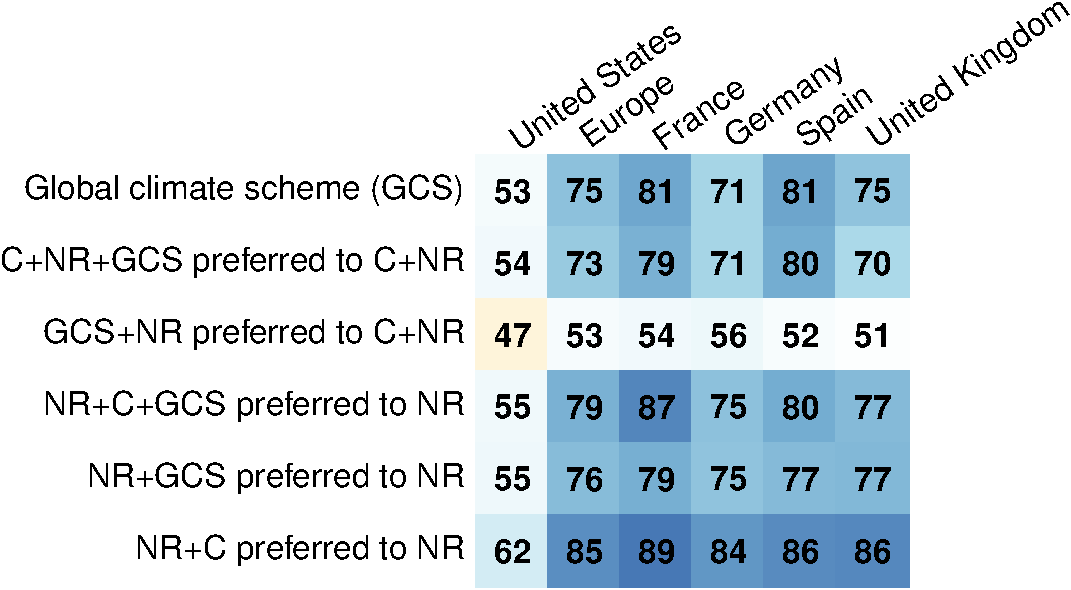
\includegraphics[height=.65\textheight]{../figures/country_comparison/conjoint_ab_positive.pdf} 
    \end{figure}
\end{frame}

\begin{frame}{Conjoint analyses: influence on preferred platform (Eu) \hyperlink{conjoint_r_uk}{\beamergotobutton{Go back}}\label{conjoint_r_eu}} 
    \begin{figure}\vspace{-.2cm}
        \centering 
        \caption{%Imagine that a [Left or Center-left coalition wins the next elections]. Here are two possible platforms on which [the coalition] may campaign (the policies in each platform are randomly drawn from a pool of credible [Left/Center-left] policies).\\
		(...) Even if you do not support the Left, which of these platforms do you prefer? 
		%\\ ~[FR: Left or center-left; DE: rot-rot-grüne; ES: PSOE; UK: Labour]
		}
        \vspace{-.2cm} 
        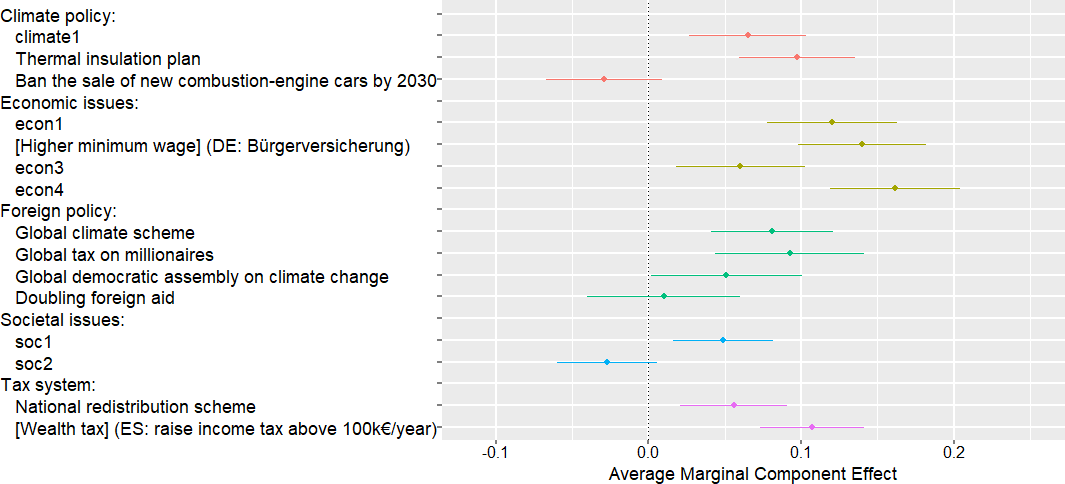
\includegraphics[height=.7\textheight]{../figures/EU/ca_r.png} 
    \end{figure}
    \bbvs \ip \rose{Europeans prefer platforms that include the GCS} and without the ban on thermal cars (a planned policy).
	\ip The effect of GCS is among the highest (wealth tax, better public services, higher minimum wage).
    \ee
\end{frame}

\begin{frame}{Conjoint analyses: influence on preferred platform (France)\label{conjoint_r_fr} \hyperlink{conjoint_r_uk}{\beamergotobutton{Go back}}} 
	\vspace{-.2cm}
    \bbvs \ip France shows that there can be a \rose{mismatch between preferred} policies (insulation plan, public services, global tax, GCS) \rose{and enacted policies} (higher retirement age and ban on thermal cars: the least preferred).
    \ee
    \begin{figure}\vspace{-.4cm}
        \centering 
        \caption{Imaginez que la gauche ou le centre gauche gagne les prochaines élections en 2027. Voici deux programmes possibles sur lesquels elle pourrait faire campagne (...)%(les mesures de ces programmes sont tirés aléatoirement depuis un ensemble de mesures de gauche ou centre gauche).
		%\\ Même si vous n'êtes pas de gauche ou centre gauche
		, lequel de ces programmes préférez-vous ?}
        \vspace{-.2cm} 
        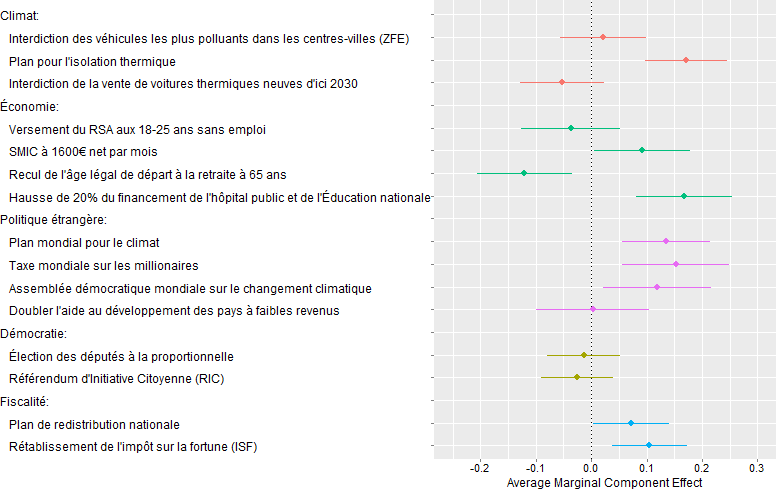
\includegraphics[height=.7\textheight]{../figures/FR/ca_r.png} 
    \end{figure}
\end{frame}

\begin{frame}{Conjoint analyses: influence on preferred platform (U.S.) \hyperlink{conjoint_r_uk}{\beamergotobutton{Go back}}\label{conjoint_r_us}} 
    \bbvs \ip \rose{Endorsing the GCS is not determinant to gain the Democratic primary.}
    \ee
    \begin{figure}\vspace{-.4cm}
        \centering 
        \caption{[Only on non-Republican] Imagine that at the 2024 Democratic party presidential primaries, the two main candidates campaign with the following key policies in their platforms.\\
		Which of these candidates do you prefer?}
        \vspace{-.2cm} 
        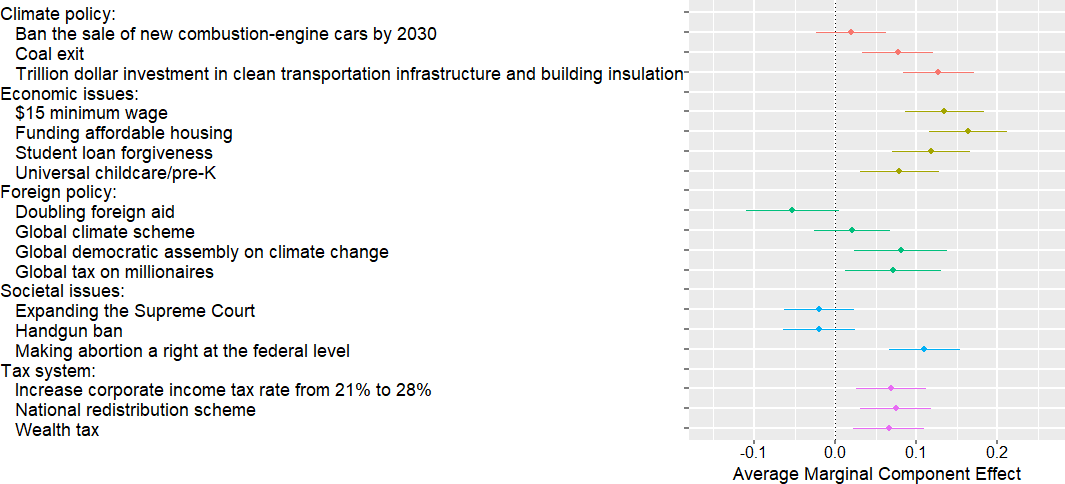
\includegraphics[height=.7\textheight]{../figures/US1/ca_r.png} 
    \end{figure}
\end{frame}

\begin{frame}{Conjoint analyses: influence on preferred platform (Germany) \hyperlink{conjoint_r_uk}{\beamergotobutton{Go back}}\label{conjoint_r_de}} 
    \bbvs \ip \rose{Endorsing the GCS is not determinant to gain the Democratic primary.}
    \ee
    \begin{figure}\vspace{-.4cm}
        \centering 
        \caption{Imagine that a Rot-Rot-Grüne coalition wins the next elections. Here are two possible platforms on which the coalition may campaign (the policies in each platform are randomly drawn from a pool of credible left-wing policies).\\
		(...) Even if you do not support the Left, which of these platforms do you prefer? }
        \vspace{-.2cm} 
        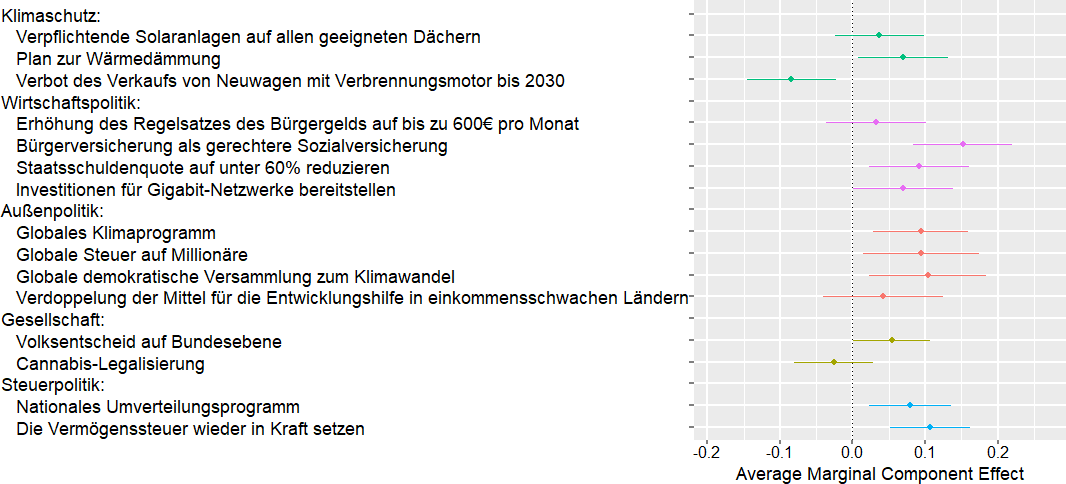
\includegraphics[height=.7\textheight]{../figures/DE/ca_r.png} 
    \end{figure}
\end{frame}

\begin{frame}{Conjoint analyses: influence on preferred platform (Spain) \hyperlink{conjoint_r_uk}{\beamergotobutton{Go back}}\label{conjoint_r_es}} 
    \bbvs \ip \rose{Endorsing the GCS is not determinant to gain the Democratic primary.}
    \ee
    \begin{figure}\vspace{-.4cm}
        \centering 
        \caption{Imagine that the PSOE wins the next elections. Here are two possible platforms on which it may campaign (the policies in each platform are randomly drawn from a pool of credible PSOE policies).\\
		(...) Even if you do not support the PSOE, which of these platforms do you prefer? }
        \vspace{-.2cm} 
        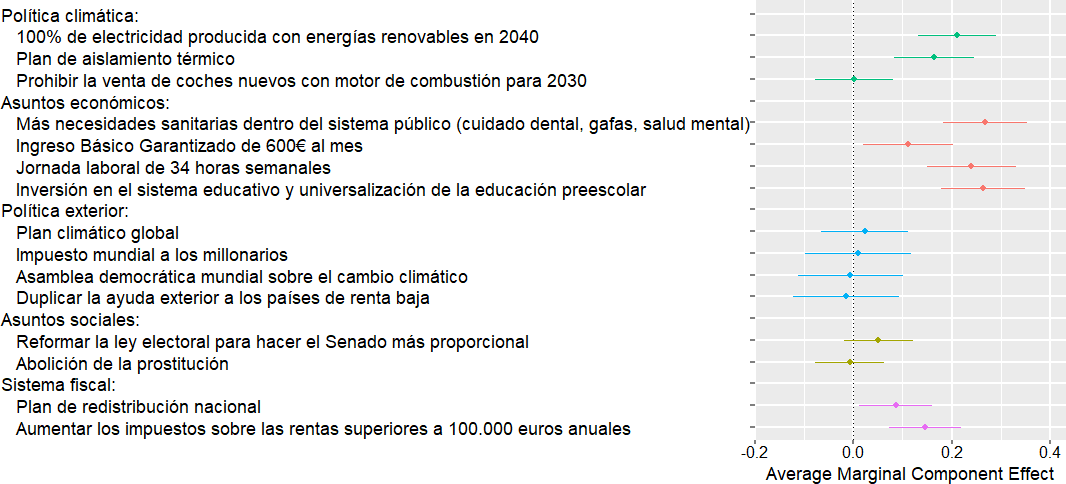
\includegraphics[height=.7\textheight]{../figures/ES/ca_r.png} 
    \end{figure}
\end{frame}

\begin{frame}{Prioritization \hyperlink{donation}{\beamergotobutton{Go back}}\label{prioritization}}
    \begin{columns}
        \begin{column}{0.35\textwidth}\vspace{-1cm}
            \bbvs \ip %``In this question, 
			``you have 100 points that you can allocate to different policies. The more you give points to a policy, the more you support it.\\ % TODO: highlight synchronously
            How do you allocate the points among the following policies?'' \\~[6 policies taken at random]
            \ip GCS is as prioritized as the average policy, or even more in France and Germany. \\ It is more prioritized than some planned climate policies, like the ban on thermal cars.
            \ip The global tax on millionaires is among the most prioritized measures.\\ It as prioritized as a national wealth tax, if not more.
            \ip Most prioritized are better public services and a higher minimum wage.
            \ee        % TODO!? everywhere, put interpretation after figures
        \end{column}
        \begin{column}{0.65\textwidth}\vspace{-.6cm}
            \begin{figure}
                \centering 
                \caption{\quad ~ \quad ~ \quad Mean number of points}
                \vspace{-.3cm}
                \includegraphics[width=\columnwidth]{../figures/country_comparison/points_mean.pdf} 
            \end{figure}
        \end{column}
    \end{columns}
\end{frame}

\begin{frame}{International climate negotiations \hyperlink{donation}{\beamergotobutton{Go back}}\label{negotiation}}
    \begin{figure}
        \centering 
        \caption{In international climate negotiations, would you prefer [U.S.] diplomats to defend [U.S.] interests or global justice?
        }
        \vspace{-.2cm}
        \includegraphics[width=\textwidth]{../figures/all/negotiation.pdf} 
    \end{figure}
	\bbvs \ip The typical answer is to defend one's country's ``interests, to the extent it respects global justice.''
    \ip Only one eigth wants to defend one's country's ``interests, even if it goes against global justice.''
    \ee
\end{frame}

\begin{frame}{Group defended \hyperlink{donation}{\beamergotobutton{Go back}}\label{group_defended}}
    \begin{figure}
        \centering 
        \caption{What group do you defend when you vote?
        }
        \vspace{-.2cm}
        \includegraphics[width=\textwidth]{../figures/all/group_defended_agg2.pdf} 
    \end{figure}
	\bbvs \ip The most defended group is one's fellow citizens.
    \ip \blue{$~$40\% are universalist}, i.e. defend all humans or sentient beings.
    \ee
\end{frame}

\begin{frame}{Biggest issues \hyperlink{donation}{\beamergotobutton{Go back}}\label{problems}}
    \begin{figure}
        \centering 
        \caption{To what extent do you think the following issues are a problem? \textit{5-Likert scale} \\(Mean of answers recoded in [-2, +2])
        }
        \vspace{-.2cm}
        \includegraphics[width=.7\textwidth]{../figures/country_comparison/problem_mean.pdf} 
    \end{figure}
	\bbvs \ip People rank these the importance of these 3 issures as follows: \\ 1. Climate change \\ 2. Global poverty \\ 3. Income inequality in their country
    \ee
\end{frame}

\begin{frame}{Eu questionnaire \hyperlink{questionnaires}{\beamergotobutton{Go back}}\label{survey_flow}}
    \vspace{.05cm}
    %\makebox[\textwidth][c]{ 
    %\begin{itemize}[<+>]
    \makebox[\textwidth][c]{ \includegraphics[height=.95\textheight]{../questionnaire/survey_flow_EU.pdf}}
    %\end{itemize}
    %}
\end{frame}

% \subsection{Representativeness}

% 	\begin{frame}{Summary statistics\label{representativeness}}	
% 		\begin{table}[h!]
% 			\caption{Summary Statistics -- High-income countries 1 }
% 				\begin{center}
% 					\scalebox{0.6}{\input{"../tables/sample_composition/AU_CA_DK_FR_ageCombined.tex"}}
% 				\end{center}
% 			\end{table}	
% 	\end{frame}

% 	\begin{frame}{Summary statistics}	
% 		\begin{table}[h!]
% 			\caption{Summary Statistics -- High-income countries 2 \hyperlink{data_quality}{\beamergotobutton{Go back}}}
% 				\begin{center}
% 					\scalebox{0.6}{\input{"../tables/sample_composition/DE_IT_JP_PL_ageCombined.tex"}}
% 				\end{center}
% 			\end{table}	
% 	\end{frame}
	
% \begin{frame}{Summary statistics}	
% 	\begin{table}[h!]
% 		\caption{Summary Statistics -- High-income countries 3 \hyperlink{data_quality}{\beamergotobutton{Go back}}}
% 			\begin{center}
% 				\scalebox{0.6}{\input{"../tables/sample_composition/SK_SP_UK_US_ageCombined.tex"}}
% 			\end{center}
% 		\end{table}	
% \end{frame}

\subsection{Descriptive statistics}


\begin{frame}{Main attitudes by vote \hyperlink{gcs_support}{\beamergotobutton{Go back}}\label{gcs_vote}}
    \begin{figure}[h!] 
        \caption{Main attitudes by vote (``Right'' spans from Center-right to Far right). (Relative support in percent)}\label{fig:main_by_vote}
        \makebox[\textwidth][c]{\includegraphics[width=.7\textwidth]{../figures/country_comparison/main_all_by_vote_share.pdf}} 
    \end{figure}
\end{frame}

\begin{frame}{Main attitudes by vote \hyperlink{gcs_support}{\beamergotobutton{Go back}}\label{gcs_vote}} % TODO: Yes on left
    \begin{figure}[h!] 
        \only<1>{\caption{Main attitudes by vote in France}
        \includegraphics[width=.7\textwidth]{../figures/FR/vote/gcs_support.pdf}}
        \only<2>{\caption{Main attitudes by vote in Germany}
        \includegraphics[width=.7\textwidth]{../figures/DE/vote/gcs_support.pdf}}
        \only<3>{\caption{Main attitudes by vote in Spain}
        \includegraphics[width=.7\textwidth]{../figures/ES/vote/gcs_support.pdf}}
        \only<4>{\caption{Main attitudes by vote in the UK}
        \includegraphics[width=.7\textwidth]{../figures/UK/vote/gcs_support.pdf}}
    \end{figure}
\end{frame}

\begin{frame}{Comprehension of the policies}\label{understanding}
    \begin{figure}[h!]
        \caption[Comprehension]{Correct answers to comprehension questions (in percent). \hyperlink{gcs_support}{\beamergotobutton{Go back}}}\label{fig:understood_each}
        \includegraphics[width=\textwidth]{../figures/country_comparison/understood_each_positive.pdf}
    \end{figure}    
\end{frame}

\begin{frame}{Comprehension of the policies}
\begin{figure}[h!]
    \caption[Comprehension score]{Number of correct answers to comprehension questions (mean). \hyperlink{gcs_support}{\beamergotobutton{Go back}}}\label{fig:understood_score}
    \includegraphics[width=\textwidth]{../figures/country_comparison/understood_score_mean.pdf} 
\end{figure}
\end{frame}

% 
% 
% \subsection{Socio-Demographics}
% \begin{frame}{Education}%\addtocounter{framenumber}{-1} % 
%     \hspace{.2cm}
% \begin{figure}[h!]
% \centering
% \caption{What is the highest level of education you have completed?}
% \includegraphics[width=.78\paperwidth]{../../oecd_climate/figures/all/education_ALL} \\
% \vspace{.3cm}
% \includegraphics[width=.78\paperwidth]{../../oecd_climate/figures/all/diploma_ALL}
% %\caption{What race or ethnicity do you identify with? (Multiple answers are possible)} % 
% %\includegraphics[width=.43\paperwidth]{../../oecd_climate/figures/all/race_ALL}\\
% \end{figure}
% \end{frame} % 
% 
% \begin{frame}{Left-right leaning}%\addtocounter{framenumber}{-1}
% \begin{figure}[h!]
% \centering
% \caption{On economic policy matters, where do you see yourself on the liberal/conservative spectrum?}
% \includegraphics[width=.87\paperwidth]{../../oecd_climate/figures/all/left_right_ALL} \\
% \end{figure}
% \end{frame}
% 
% \begin{frame}{Geography}%\addtocounter{framenumber}{-1}
% \begin{figure}[h!]
% \centering
% \caption{Lives in an urban area (town > 20k people), retrieved from zipcode}
% \includegraphics[width=.8\paperwidth]{../../oecd_climate/figures/all/urbanity_ALL.png} \\
% \vspace{.2cm}
% %\caption{Region, retrieved from zipcode} % 
% %\includegraphics[width=.43\paperwidth]{../../oecd_climate/figures/all/region_ALL}
% \end{figure}
% \end{frame}

% \begin{frame}{Gender and age}%\addtocounter{framenumber}{-1}
% \begin{figure}[h!]
% \centering
% \caption{What is your gender?}
% \includegraphics[width=.6\paperwidth]{../../oecd_climate/figures/all/gender_ALL} \\
% \centering
% \caption{How old are you?}
% \includegraphics[width=.6\paperwidth]{../../oecd_climate/figures/all/age_ALL}
% \end{figure}
% \end{frame}
% \subsection{Household %Composition and Energy 
% Characteristics}

% \begin{frame}{Income/wealth}%\addtocounter{framenumber}{-1}
% \begin{figure}[h!]
% \centering
% \captionsetup{justification=centering}
% \caption{What was the annual income of your household in 2019 (before withholding tax, for you and those who live with you)?}
% \includegraphics[width=.43\paperwidth]{../../oecd_climate/figures/all/income_ALL} \\
% \caption{\small What is the estimated value of your assets, or the assets of your household if you are married (in [currency])? Include here all your possessions (home, car, savings, etc.) net of debt. For example, if you own a house worth \$300,000 and you have \$100,000 left to repay on your mortgage, your assets are \$200,000.}
% \includegraphics[width=.43\paperwidth]{../../oecd_climate/figures/all/wealth_ALL} \\
% \end{figure}
% \end{frame}


% \subsection{Political leaning}

% \begin{frame}{Little interest for politics}%\addtocounter{framenumber}{-1}
% \vspace{-.5cm}
% \begin{figure}[h!]
% \caption{To what extent are you interested in politics?}
% \includegraphics[width=.52\paperwidth]{../../oecd_climate/figures/all/interested_politics_ALL} \\
% %\caption{Could you trust the federal goverment to implement the following policies}
% \vspace{.1cm}
% \caption{Are you member of an environmental organization?}
% \includegraphics[width=.47\paperwidth]{../../oecd_climate/figures/all/member_environmental_orga_ALL}\\
% \vspace{.1cm}
% \caption{Do you have any relatives who are environmentalists?}
% \includegraphics[width=.47\paperwidth]{../../oecd_climate/figures/all/relative_environmentalist_ALL}\\
% \end{figure}
% \end{frame}

% \begin{frame}{Broadly representative political leaning}%\addtocounter{framenumber}{-1}
% \vspace{-.5cm}
% \begin{figure}[h!]
% \caption{Did you vote in the [last Country] election?}
% \includegraphics[width=.45\paperwidth]{../../oecd_climate/figures/all/vote_participation_ALL} \\
% %\caption{Could you trust the federal goverment to implement the following policies}
% \vspace{.1cm}
% \caption{Which candidate did you vote / would you have voted for in the last presidential election?}
% \includegraphics[width=.7\paperwidth]{../../oecd_climate/figures/all/vote_main_ALL} \\
% \caption{On economic policy matters, where do you see yourself on the left/right spectrum?}
% \includegraphics[width=.7\paperwidth]{../../oecd_climate/figures/all/left_right_ALL}
% % \caption{Which candidate did you vote for in the last presidential election?}
% % \includegraphics[width=.52\paperwidth]{../../oecd_climate/figures/all/vote_all_ALL} \\
% % \caption{Did you vote in the 2016 [country] presidential election?}
% % \includegraphics[width=.47\paperwidth]{../../oecd_climate/figures/all/vote_participation_2016_ALL}\\
% \end{figure}
% \end{frame}

\subsection{Distributive effects of the Global Climate Plan}

\begin{frame}{Distributive effects of the Global Climate Plan\label{other_distributive} \hyperlink{distributive}{\beamergotobutton{Go back}}}
    \begin{figure}
        \centering 
        \only<1>{ \caption{Distributive effects of the Global Climate Plan in 2030.}
        \includegraphics[height=.8\textheight]{../figures/maps/gain_adj_2030.pdf}}
        \only<2>{ \caption{Distributive effects of the Global Climate Plan in 2040.}
        \includegraphics[height=.8\textheight]{../figures/maps/gain_adj_2040.pdf}}
        \only<3>{ \caption{Distributive effects of the Global Climate Plan in 2050.}
        \includegraphics[height=.8\textheight]{../figures/maps/gain_adj_2050.pdf}}
        \only<4>{ \caption{Distributive effects of the Global Climate Plan in 2060.}
        \includegraphics[height=.8\textheight]{../figures/maps/gain_adj_2060.pdf}}
        \only<5>{ \caption{Distributive effects of the Global Climate Plan in 2070.}
        \includegraphics[height=.8\textheight]{../figures/maps/gain_adj_2070.pdf}}
        \only<6>{ \caption{Distributive effects of the Global Climate Plan in 2080.}
        \includegraphics[height=.8\textheight]{../figures/maps/gain_adj_2080.pdf}}
    \end{figure}        
\end{frame}

\begin{frame}{Distributive effects of the Global Climate Plan \hyperlink{distributive}{\beamergotobutton{Go back}}}
    \begin{figure}
        \centering 
        \only<1>{ \caption{Distributive effects of the Global Climate Plan in 2030.}
        \includegraphics[height=.8\textheight]{../figures/maps/gain_adj_over_gdp_2030.pdf}}
        \only<2>{ \caption{Distributive effects of the Global Climate Plan in 2040.}
        \includegraphics[height=.8\textheight]{../figures/maps/gain_adj_over_gdp_2040.pdf}}
        \only<3>{ \caption{Distributive effects of the Global Climate Plan in 2050.}
        \includegraphics[height=.8\textheight]{../figures/maps/gain_adj_over_gdp_2050.pdf}}
        \only<4>{ \caption{Distributive effects of the Global Climate Plan in 2060.}
        \includegraphics[height=.8\textheight]{../figures/maps/gain_adj_over_gdp_2060.pdf}}
        \only<5>{ \caption{Distributive effects of the Global Climate Plan in 2070.}
        \includegraphics[height=.8\textheight]{../figures/maps/gain_adj_over_gdp_2070.pdf}}
        \only<6>{ \caption{Distributive effects of the Global Climate Plan in 2080.}
        \includegraphics[height=.8\textheight]{../figures/maps/gain_adj_over_gdp_2080.pdf}}
    \end{figure}        
\end{frame}

\begin{frame}{Distributive effects of the Global Climate Plan \hyperlink{distributive}{\beamergotobutton{Go back}}}
    \begin{figure}
        \centering 
        \only<1>{ \caption{Distributive effects of the Global Climate \textit{Scheme}.}
        \includegraphics[height=.8\textheight]{../figures/maps/npv_over_gdp_gcs.pdf}}
        \only<2>{ \caption{Distributive effects of the Global Climate \textit{Plan}.}
        \includegraphics[height=.8\textheight]{../figures/maps/npv_over_gdp_gcs_adj.pdf}}
        % \only<3>{ \caption{Distributive effects of the Global Climate Plan.}
        % \includegraphics[height=.8\textheight]{../figures/maps/npv_pa_gcs_adj.pdf}} % TODO! pb with this figure
    \end{figure}        
\end{frame}

\subsection{OECD\label{detail_global}}

% \begin{frame}{Quasi-unanimous agreement on need for global policies}%\addtocounter{framenumber}{-1}
% \vspace{-1cm}
% \begin{figure}[h!]
% \centering
% \caption{\small{At which level(s) do you think public policies to tackle climate change need to be put in place? (Multiple answers are possible)}}
% \includegraphics[width=.43\paperwidth]{../../oecd_climate/figures/all/scale_ALL}
% \end{figure}
% \end{frame}

% \begin{frame}{Large support for international transfers}%\addtocounter{framenumber}{-1}
% \begin{figure}[h!]
% \centering
% \caption{To achieve a given reduction of greenhouse gas emissions globally, costly investments are needed.
% Ideally, how should countries bear the costs of fighting climate change?}
% \vspace{2mm}
% % TODOO \includegraphics[width=.95\paperwidth]{../../oecd_climate/figures/all/burden_sharing_ALL}
% %\caption{}
% \end{figure}
% \end{frame}

% \begin{frame}{Large support for a fairer global order}%\addtocounter{framenumber}{-1}
% \begin{figure}[h!]
% \centering
% \caption{Do you support or oppose the following policies?}
% \vspace{2mm}
% \includegraphics[width=.87\paperwidth]{../../oecd_climate/figures/all/global_policies_ALL}
% %\caption{}
% \end{figure}
% \end{frame}

\begin{frame}{Relative support for national policies\label{national_policies} \hyperlink{global_policies}{\beamergotobutton{Go back}}} 
    % National vs. global support: global T&D < national T&D << GCS (except in U.S. where the three are equally supported)
	\begin{figure}[h!]
	\centering
	%\caption{Relative support for national policies}
	\includegraphics[height=.8\paperheight]{../../oecd_climate/figures/country_comparison/Heatplot_national_policies_share_countries.pdf}
	\end{figure}
    Support in high-income countries: Global tax and dividend $\lesssim$ National tax and dividend $<$ Global quota and dividend \\ Except in the U.S. where the three are equally supported.
\end{frame}

\begin{frame}{Absolute support for global policies\label{absolute_oecd} \hyperlink{global_policies}{\beamergotobutton{Go back}}} 
\begin{figure}[h!]
    \centering		
    \caption{Share of support (somewhat or strongly) for the main global policies among non-\textit{indifferent}.   }
    \vspace{-.2cm}
    \includegraphics[height=.82\textheight]{../figures/OECD/Heatplot_global_tax_attitudes_positive.pdf} % burden_share_all_share_countries
    \end{figure}
\end{frame}

\begin{frame}{} % TODOO
	\begin{figure}[h!]
	\centering
	\caption{Do you agree or disagree with the following statement: ``[country] should take measures to fight climate change.'' \hyperlink{global_policies}{\beamergotobutton{Go back}}
	%Pourcentage de réponses (plutôt ou très favorable) parmi~:	Très opposé$\cdot$e; Plutôt opposé$\cdot$e; Indifférent$\cdot$e; Plutôt favorable; Très favorable
	}
% \item 
% 	\\ \textit{Strongly disagree; Somewhat disagree; Neither agree nor disagree; Somewhat agree; Strongly agree}
	\includegraphics[height=.8\paperheight]{../../oecd_climate/figures/country_comparison/should_fight_CC_countries.pdf}
	\end{figure}
\end{frame}

\begin{frame}{}%\addtocounter{framenumber}{-1}
	\begin{figure}[h!]
	\centering
	\caption{
		At which level(s) do you think public policies to tackle climate change need to be put in place? (Multiple answers are possible) \hyperlink{global_policies}{\beamergotobutton{Go back}}
		%\\ En France, les options sont~: Mondiale; Européenne; Nationale; Locale; 
	}
		% \begin{enumerate}[resume] \item 
% \\ \textit{Global; [Federal / European / ...]; [State / National]; Local}
	\includegraphics[width=\paperwidth]{../../oecd_climate/figures/country_comparison/scale_positive_countries.pdf}
	\end{figure}
\end{frame}

\begin{frame}{}
	\begin{figure}[h!]
	\centering
	\caption{How should [country] climate policies depend on what other countries do? \\
	If other countries do more, [country] should do... \hyperlink{global_policies}{\beamergotobutton{Go back}}
	%Pourcentage de réponse \textit{Plus} ou \textit{Beaucoup plus} parmi~: Beaucoup moins; Moins; À peu près autant; Plus; Beaucoup plus. 
	}
	% \item How should [country] climate policies depend on what other countries do?
% 	\begin{itemize}
% \item If other countries do more, [country] should do…
% \item If other countries do less, [country] should do…
% \end{itemize}
% \textit{Much less; Less; About the same; More; Much more}
	\includegraphics[height=.8\paperheight]{../../oecd_climate/figures/country_comparison/if_other_do_more_countries.pdf}
	\end{figure}
\end{frame}

\begin{frame}{}
	\begin{figure}[h!]
	\centering
	\caption{How should [country] climate policies depend on what other countries do? \\
	If other countries do less, [country] should do... \hyperlink{global_policies}{\beamergotobutton{Go back}}
	%Pourcentage de réponse \textit{Plus} ou \textit{Beaucoup plus} parmi~: Beaucoup moins; Moins; À peu près autant; Plus; Beaucoup plus.
	% Si d'autres pays en font plus, la France devrait en faire...
	}
	% \item How should [country] climate policies depend on what other countries do?
% 	\begin{itemize}
% \item If other countries do more, [country] should do…
% \item If other countries do less, [country] should do…
% \end{itemize}
% \textit{Much less; Less; About the same; More; Much more}
	\includegraphics[height=.8\paperheight]{../../oecd_climate/figures/country_comparison/if_other_do_less_countries.pdf}
	\end{figure}
\end{frame}

% \begin{frame}{}
% 	\begin{figure}[h!]
% 	\centering
% 	\caption{[Question posée seulement aux U.S., au Danemark et en France; ici résultats pour la France] Pour parvenir à une réduction donnée des émissions de gaz à effet de serre au niveau mondial, de coûteux investissements sont nécessaires. \\
% 	Dans l'idéal, comment les pays devraient-ils répartir les coûts de la lutte contre le changement climatique ? \\
% 	Pourcentage de réponses (plutôt ou très favorable) parmi~:	Très opposé$\cdot$e; Plutôt opposé$\cdot$e; Indifférent$\cdot$e; Plutôt favorable; Très favorable
% 	% Les pays devraient payer en proportion de leur richesse
% 	% Les pays devraient payer en proportion de leurs émissions actuelles
% 	% Les pays devraient payer en proportion de leurs émissions passées (à partir de 1990)
% 	% Les pays les plus riches devraient payer davantage, afin que les pays les plus pauvres n'aient pas à payer
% 	% Les pays les plus riches devraient payer beaucoup plus, pour aider les pays vulnérables à faire face aux conséquences néfastes : les pays vulnérables recevraient de l'argent au lieu de payer
% 	}
% % \\ \textit{Strongly oppose; Somewhat oppose; Neither support nor oppose; Somewhat support; Strongly support}
% % \item ~[In all countries but the U.S., Denmark and France] Suppose the above policy is in place. How should the carbon budget be divided among countries?
% % \\ \textit{The emission share of a country should be proportional to its population, so that each human has an equal right to emit.; The emission share of a country should be proportional to its current emissions, so that those who already emit more have more rights to emit.; Countries that have emitted more over the past decades (from 1990 onwards) should receive a lower emission share, because they have already used some of their fair share.; Countries that will be hurt more by climate change should receive a higher emission share, to compensate them for the damages.}
% % \item ~[In the U.S., Denmark, and France only] To achieve a given reduction of greenhouse gas emissions globally, costly investments are needed.
% % Ideally, how should countries bear the costs of fighting climate change?
% % 	\begin{itemize}
% % \item Countries should pay in proportion to their income
% % \item Countries should pay in proportion to their current emissions
% % \item Countries should pay in proportion to their past emissions (from 1990 onwards)
% % \item The richest countries should pay it all, so that the poorest countries do not have to pay anything
% % \item The richest countries should pay even more, to help vulnerable countries face adverse consequences: vulnerable countries would then receive money instead of paying
% % \end{itemize} 
% % \textit{Strongly disagree; Somewhat disagree; Neither agree nor disagree; Somewhat agree; Strongly agree}
% 	\includegraphics[width=\textwidth]{../../oecd_climate/figures/FR/burden_sharing_FR.png}
% 	\end{figure}
% \end{frame}

\begin{frame}{}
	\begin{figure}[h!]
	\centering
	\caption{\scriptsize [Question non posée aux U.S., au Danemark et en France]  All countries have signed the Paris agreement that aims to contain global warming ``well below +2 \textdegree{}C''. To limit global warming to this level, there is a maximum amount of greenhouse gases we can emit globally, called the carbon budget. Each country could aim to emit less than a share of the carbon budget. To respect the global carbon budget, countries that emit more than their national share would pay a fee to countries that emit less than their share. \\ 
	Do you support such a policy? \hyperlink{global_policies}{\beamergotobutton{Go back}}
	}
	\includegraphics[height=.7\paperheight]{../../oecd_climate/figures/country_comparison/global_quota_countries.pdf}
	\end{figure}
\end{frame}

\begin{frame}{}
	\begin{figure}[h!]
	\centering
	\caption{[*Question not asked in the U.S., Denmark and France, answers to a similar question are displayed] \\ Suppose the above policy is in place. How should the carbon budget be divided among countries?
	\\ The emission share of a country should be proportional to its population, so that each human has an equal right to emit.; The emission share of a country should be proportional to its current emissions, so that those who already emit more have more rights to emit.; Countries that have emitted more over the past decades (from 1990 onwards) should receive a lower emission share, because they have already used some of their fair share.; Countries that will be hurt more by climate change should receive a higher emission share, to compensate them for the damages. \\
	Percentage of support (somewhat or strong) among: \textit{Strongly oppose; Somewhat oppose; Neither support nor oppose; Somewhat support; Strongly support} \hyperlink{global_policies}{\beamergotobutton{Go back}}
	}
	% \item Do you support or oppose establishing a global democratic assembly whose role would be to draft international treaties against climate change? Each adult across the world would have one vote to elect members of the assembly.
	\includegraphics[width=\paperwidth]{../../oecd_climate/figures/country_comparison/burden_share_positive_countries.pdf}
	\end{figure}
\end{frame}

\begin{frame}{}
	\begin{figure}[h!]
	\centering
	\caption{ Do you support or oppose establishing a global democratic assembly whose role would be to draft international treaties against climate change? Each adult across the world would have one vote to elect members of the assembly. \hyperlink{global_policies}{\beamergotobutton{Go back}}
	%\\ Pourcentage de réponses (plutôt ou très favorable) parmi~:	Très opposé$\cdot$e; Plutôt opposé$\cdot$e; Indifférent$\cdot$e; Plutôt favorable; Très favorable}
	% \item 
% \\ \textit{Strongly oppose; Somewhat oppose; Neither support nor oppose; Somewhat support; Strongly support
}
	\includegraphics[height=.8\paperheight]{../../oecd_climate/figures/country_comparison/global_assembly_support_countries.pdf}
	\end{figure}
\end{frame}

\begin{frame}{}
	\begin{figure}[h!]
	\centering \vspace{-.3cm}
	\caption{\scriptsize Imagine the following policy: a global tax on greenhouse gas emissions funding a global basic income. 
	Such a policy would progressively raise the price of fossil fuels (for example, the price of gasoline would increase by [40 cents per gallon] in the first years). Higher prices would encourage people and companies to use less fossil fuels, reducing greenhouse gas emissions. Revenues from the tax would be used to finance a basic income of [\$30] per month to each human adult, thereby lifting the 700 million people who earn less than \$2/day out of extreme poverty. 
	The average British person would lose a bit from this policy as they would face [\$130] per month in price increases, which is higher than the [\$30] they would receive.
	\\
	Do you support or oppose such a policy?   \hyperlink{global_policies}{\beamergotobutton{Go back}}
	%Pourcentage de réponses (plutôt ou très favorable) parmi~:	Très opposé$\cdot$e; Plutôt opposé$\cdot$e; Indifférent$\cdot$e; Plutôt favorable; Très favorable
	}
% \\ \textit{Strongly oppose; Somewhat oppose; Neither support nor oppose; Somewhat support; Strongly support}
	\includegraphics[height=.65\paperheight]{../../oecd_climate/figures/country_comparison/global_tax_support_countries.pdf}
	\end{figure}
\end{frame}

\begin{frame}{}
	\begin{figure}[h!]
	\centering
	\caption{\scriptsize Do you support or oppose a tax on all millionaires around the world to finance low-income countries that comply with international standards regarding climate action? 
	This would finance infrastructure and public services such as access to drinking water, healthcare, and education.  \hyperlink{global_policies}{\beamergotobutton{Go back}}
	%Pourcentage de réponses (plutôt ou très favorable) parmi~:	Très opposé$\cdot$e; Plutôt opposé$\cdot$e; Indifférent$\cdot$e; Plutôt favorable; Très favorable
	}
	% \item D
% \\ \textit{Strongly oppose; Somewhat oppose; Neither support nor oppose; Somewhat support; Strongly support}
	\includegraphics[height=.8\paperheight]{../../oecd_climate/figures/country_comparison/tax_1p_support_countries.pdf}
	\end{figure}
\end{frame}
	
\begin{frame}{}%\addtocounter{framenumber}{-1}
	\begin{figure}[h!]
	\centering
	\caption{Synthèse~: Pourcentage de réponses positive (e.g. Plutôt/Très favorable). \hyperlink{global_policies}{\beamergotobutton{Go back}}}
	\includegraphics[width=\paperwidth]{../../oecd_climate/figures/country_comparison/burden_share_all_positive_countries.pdf}
	%\caption{}
	\end{figure}
\end{frame}

\begin{frame}{}%\addtocounter{framenumber}{-1}
	\begin{figure}[h!]
	\centering
	\caption{Synthèse~: Pourcentage de réponses positive (e.g. \textit{Plutôt/Très favorable}) parmi les non \textit{indifférents}. \hyperlink{global_policies}{\beamergotobutton{Go back}}}
	\includegraphics[width=\paperwidth]{../../oecd_climate/figures/country_comparison/burden_share_all_share_countries.pdf}
	%\caption{}
	\end{figure}
\end{frame}

	
\begin{frame}{Principales des attitudes sur les politiques mondiales}%\addtocounter{framenumber}{-1}
	\begin{figure}[h!]
	\centering
	\caption{Pourcentage de réponses positive (e.g. Plutôt/Très favorable). \hyperlink{global_policies}{\beamergotobutton{Go back}}}
	\includegraphics[width=\paperwidth]{../../oecd_climate/figures/country_comparison/burden_share_few_positive_countries.pdf}
	%\caption{}
	\end{figure}
\end{frame}

\begin{frame}{Principales attitudes sur les politiques mondiales}%\addtocounter{framenumber}{-1}
	\begin{figure}[h!]
	\centering
	\caption{Pourcentage de réponses positive (e.g. \textit{Plutôt/Très favorable}) parmi les non \textit{indifférents}. \hyperlink{global_policies}{\beamergotobutton{Go back}}}
	\includegraphics[width=\paperwidth]{../../oecd_climate/figures/country_comparison/burden_share_few_share_countries.pdf}
	%\caption{}
	\end{figure}
\end{frame}

\begin{frame}{Principales attitudes sur les politiques mondiales}%\addtocounter{framenumber}{-1}
	\begin{figure}[h!]
	\centering
	\caption{Moyennes des réponses, recodées en [$-$2; +2]. \hyperlink{global_policies}{\beamergotobutton{Go back}}}
	\includegraphics[width=\paperwidth]{../../oecd_climate/figures/country_comparison/burden_share_few_mean_countries.pdf}
	%\caption{}
	\end{figure}
\end{frame}

\end{framefont}


\end{document}